\documentclass[12pt]{ociamthesis}  % default square logo 
%\documentclass[12pt,beltcrest]{ociamthesis} % use old belt crest logo
%\documentclass[12pt,shieldcrest]{ociamthesis} % use older shield crest logo

%load any additional packages
\usepackage{amssymb}
\usepackage{graphicx}
\usepackage[utf8]{inputenc}
\usepackage[english]{babel}
\usepackage{csquotes}
\usepackage{xspace}
\usepackage{url}
\usepackage{bookmark}
\usepackage{hyperref}
\hypersetup{
    colorlinks=true,
    linkcolor=black,
    filecolor=black,      
    urlcolor=blue,
}
\usepackage{amsmath}
\usepackage{mathrsfs}
\usepackage{subcaption}
\usepackage{listings}

\usepackage{amsfonts}
\usepackage{float}
\usepackage{multirow}

\usepackage[utf8]{inputenc}
\usepackage[T1]{fontenc}

\usepackage{mathtools}

\usepackage{epstopdf}
\usepackage{manfnt}
\reversemarginpar
%\usepackage{showframe}% debugging tool
\usepackage{xcolor}
\usepackage{bm}
\usepackage{caption}
\usepackage{subcaption}
\usepackage{wrapfig} 
\usepackage{textcomp}
\usepackage{xspace}
\usepackage{mathrsfs}
\usepackage{nicefrac}
\usepackage{rotating}
\usepackage{bibentry}
\usepackage{biblatex}
\usepackage[capitalise]{cleveref}
\usepackage{enumitem}
\setlist[enumerate]{label*=\arabic*.}

\addbibresource{refs.bib}

\lstset{frame=tb, 
escapeinside={(*@}{@*)}}
\graphicspath{ {./assets/images/} }

%input macros (i.e. write your own macros file called mymacros.tex 
%and uncomment the next line)
% \def\AB{{A$\beta$}\xspace}
% \def\TP{{$\tau$P}\xspace}

% \def\div{\nabla\cdot}
% \def\grad{\nabla}
% \newcommand{\tns}[1]{\mathbf{#1}}
% \newcommand{\vc}[1]{\mathbf{#1}}
% \newcommand{\pdl}[2]{\frac{\partial\,#1}{\partial\,#2}}
% \newcommand{\de}[2]{\frac{d\,#1}{d\,#2}}
% \newcommand{\pds}[2]{\partial_{#2}#1}


\def\AB{{A$\beta$}\xspace}
\def\TP{{$\tau$P}\xspace}
\def\p0{$\mathbf{p_0}$\xspace}
\def\pI{$\mathbf{p_\infty}$\xspace}
\def\ABP{$A\beta^{+}$\xspace}
\def\ABN{$A\beta^{-}$\xspace}
\def\TPP{$\tau P^{+}$\xspace}
\def\TPN{$\tau P^{-}$\xspace}

\newcommand{\tns}[1]{\mathbf{#1}}
\newcommand{\vc}[1]{\mathbf{#1}}
\newcommand{\pdl}[2]{\frac{\partial\,#1}{\partial\,#2}}
\newcommand{\pds}[2]{\partial_{#2}#1}
\newcommand{\odl}[2]{\dfrac{\mathrm{d}#1}{\mathrm{d}#2}}
\newcommand{\lap}[1]{\sum\limits_{j=1}^{N}\mathcal{L}_{ij} #1}
\newcommand{\sso}[1]{\left(s_{#1} - s_{0,#1}\right)}
\newcommand{\ssi}[1]{\left(s_{\infty, #1} - s_{0,#1}\right)}

\title{Data-Driven Mathematical Modelling of Alzheimer's Disease}   %note \\[1ex] is a line break in the title

\author{Pavan Chaggar}             %your name
\college{Exeter College}  %your college

%\renewcommand{\submittedtext}{change the default text here if needed}
\degree{Doctor of Philosophy}     %the degree
\degreedate{Michaelmas 2021}      %the degree date

%end the preamble and start the document
\begin{document}

%this baselineskip gives sufficient line spacing for an examiner to easily
%markup the thesis with comments
\baselineskip=18pt plus1pt

%set the number of sectioning levels that get number and appear in the contents
\setcounter{secnumdepth}{3}
\setcounter{tocdepth}{3}

\maketitle                  % create a title page from the preamble info
% \include{dedication}        % include a dedication.tex file
% \include{acknowlegements}   % include an acknowledgements.tex file
\begin{center}
    \vspace*{1.5cm}
    \Large \bfseries  Abstract
\end{center}

Alzheimer's disease is a devastating neurological disorder characterised by
progressive and staged grey matter atrophy, leading to a broad dwindling of
brain functions. At present, Alzheimer's disease remains incurable, with disease
modifying interventions limited. Toxic forms of two proteins, amyloid-$\beta$
(\AB) and $\tau$-protein (\TP), are believed to underlie Alzheimer's disease by
aggregating into amyloid plaques and tau tangles, which in turn cause cellular
disruption and death. The spreading of these proteins through the brain,
particularly that of tau-protein, is highly conserved among Alzheimer's patients
and is correlated with the progression of grey-matter atrophy and symptom onset.
These features have been subject to extensive modelling work over the past
decade, with results showing that simple models of protein transport and growth
are able to reproduce clinical patterns. In recent work, we have shown that a
Bayesian modelling pipeline can be applied to calibrate models with
$\tau$-protein PET data, estimate parametric uncertainty and predict patient
trajectories. However, the simple models that have been analysed with patient
data exclude important features about \TP PET observations that may bias
simulations and result in erroneous predictions for patient trajectories. To
address this issue, we develop model of \TP propagation that incorporates
important features of \TP PET, namely observed baseline and carrying capacities.
Using this regionally specific model of \TP PET, we use a Bayesian pipeline to
calibrate a population level hierarchical model for different patient groups.
Our results highlight differences in dynamics across patient groups, showing
higher rates of transport in early stage disease and faster growth rates in late
stage disease. This work provides the first generative model of \TP PET and
accurately fits the subject data across different patient groups. With a robust
model of \TP in hand, I then outline plans for future work on incorporating
other important parts of AD pathology, such as \AB interactions and genetic risk
factors.           % include the abstract

\begin{romanpages}          % start roman page numbering
\tableofcontents            % generate and include a table of contents
\listoffigures              % generate and include a list of figures
\end{romanpages}            % end roman page numbering

%now include the files of latex for each of the chapters etc
\chapter{Introduction}
\label{chp:1}
\section{Motivation}
\label{sec:1-motivation}
Alzheimer's disease (AD) is a complex neurological disorder
characterised by progressive structural brain damage and cognitive decline.
At present, AD remains incurable and difficult to treat,
placing a significant strain on those affected by the disease and society as a
whole. Despite the plentiful resources devoted to the treatment and
understanding of the diseases, the development of pharmacological interventions
has made little progress over the past several decades. Currently, research on
the aetiology of AD comprises investigation into numerous theories, including
the cholinergic hypothesis, the amyloid hypothesis and the prion-like
propagation hypothesis, among others \cite{liu2019history}. The failure to make
progress in designing effective disease altering treatments has motivated the
use of interdisciplinary investigation to help unify our knowledge of AD and
better understand its mechanisms. 

An important obstacle hindering scientific investigation of the processes
underlying Alzheimer's is the difficulty in making and understanding
observations of the disease in-vivo. It is challenging to make accurate
measurements of biological processes occurring over time in the human brain and
equally as difficult to interpret them. Over recent decades, increasingly
sophisticated technologies have been developed to image human brains, notably
positron emission tomography (PET) scanning and magnetic resonance imaging
(MRI). Brain imaging has facilitated scientists in building upon theories of AD
developed using in-vitro and in-vivo animal studies.  
In particular, neuroimaging studies have validated post-mortem studies into
protein staging \cite{Ossenkoppele2016,SCHOLL2016971,lowe2016, cho2016vivo},
patterns of atrophy \cite{jack2018nia,whitewell2010}, and changes to functional
activity \cite{chen2019functional}. Researchers have recognised the value of
these data and several open neuroimaging databases now exist to accelerate
investigation, including the Alzheimer's Disease Neuroimaging Initiative (ADNI),
the Human Connectome Project, the Swedish BioFINDER study and more, making
the process of obtaining and analysing observations less cumbersome. 

However, progress is still slow, in part because of the unyielding challenge of
modelling high dimensional neuroimaging data. This thesis aims to address this
problem through the marriage of dynamical systems and probabilistic inference.
The former allows for interpretability of high dimensional data through 
parsimonious mechanistic models; the latter
allows us to quantify the uncertainty present throughout the stages of such
modelling, from parameter identification and uncertainty to model selection. In
combination, these methods provide useful for investigation into AD by
diminishing obstacles of data interpretation. 

Interrogating AD in this way requires at least three components: biological
understanding, data, and models. Biological understanding is needed to formulate
theories and data is needed to test  
them. I will now briefly overview key features of \AB and \TP and current
methods used for making in-vivo observations in humans, before discussing the
modelling framework employed and the sources of uncertainty present.

\section{Biological Mechanisms of Alzheimer's Disease}
\label{sec:1-bio-ad}

% Several theories regarding the processes underlying AD development have been
% proposed and it continues to be an active research area. Theories include
% neurotransmitter dysfunction \cite{davies1976selective, francis1999cholinergic},
% protein aggregation
% \cite{selkoe1991molecular,hardy1991amyloid,walker2015neurodegenerative} and
% inhibited clearance of neurotoxins \cite{rasmussen2018glymphatic}. The main
% thrust of AD research in recent decades has focussed on the role of misfolded
% proteins, namely, Amyloid-$\beta$, \AB, which aggregate to form senile plaques, and
% $\tau$-protein, \TP, which aggregates into tangles
% \cite{jucker2013self,jucker2018propagation,walker2018standard}. In this section,
% I will briefly overview important results regarding these proteins and and their
% pathological mechanisms. 

A leading proposal for the the aetiology of AD is the prion-like propagation
hypothesis, which posits that pathology follows from prion-like processes of \AB
and \TP propagating and aggregating throughout the brain, causing tissue damage
and degeneration \cite{walker2015neurodegenerative, goedert2015alzheimer,
aoyagi2019abeta}. Early investigations focussed primarily on the role of \AB in
AD pathology \cite{selkoe1991molecular, hardy1991amyloid, hardy1992alzheimer,
hardy2002amyloid}, however, growing evidence suggests that both \AB and \TP are
necessary for AD pathology to \cite{selkoe2016amyloid, kametani2018reconsideration,
aoyagi2019abeta, ossenkoppele2022amyloid}.  

While \AB and \TP have different functions and properties, their toxic forms
both exhibit an ability to self-propagate by inducing conformational changes to
their healthy counterparts \cite{prusiner1991, prusiner1998,
walker2015neurodegenerative}. This prion-like property of templating begets the
ability of \AB and \TP to self-propagate. Their accumulation follows from at
least two processes: first, the aggregation of toxic \AB and \TP into senile 
plaques and tangles, respectively;
second, inhibited clearance of toxic aggregates
\cite{duyckaerts2009classification,tarasoff2015clearance}. An important part of 
modelling the evolution of \AB and \TP in the brain will rely on accurately 
describing the prion-like process.

\begin{figure}[t]
    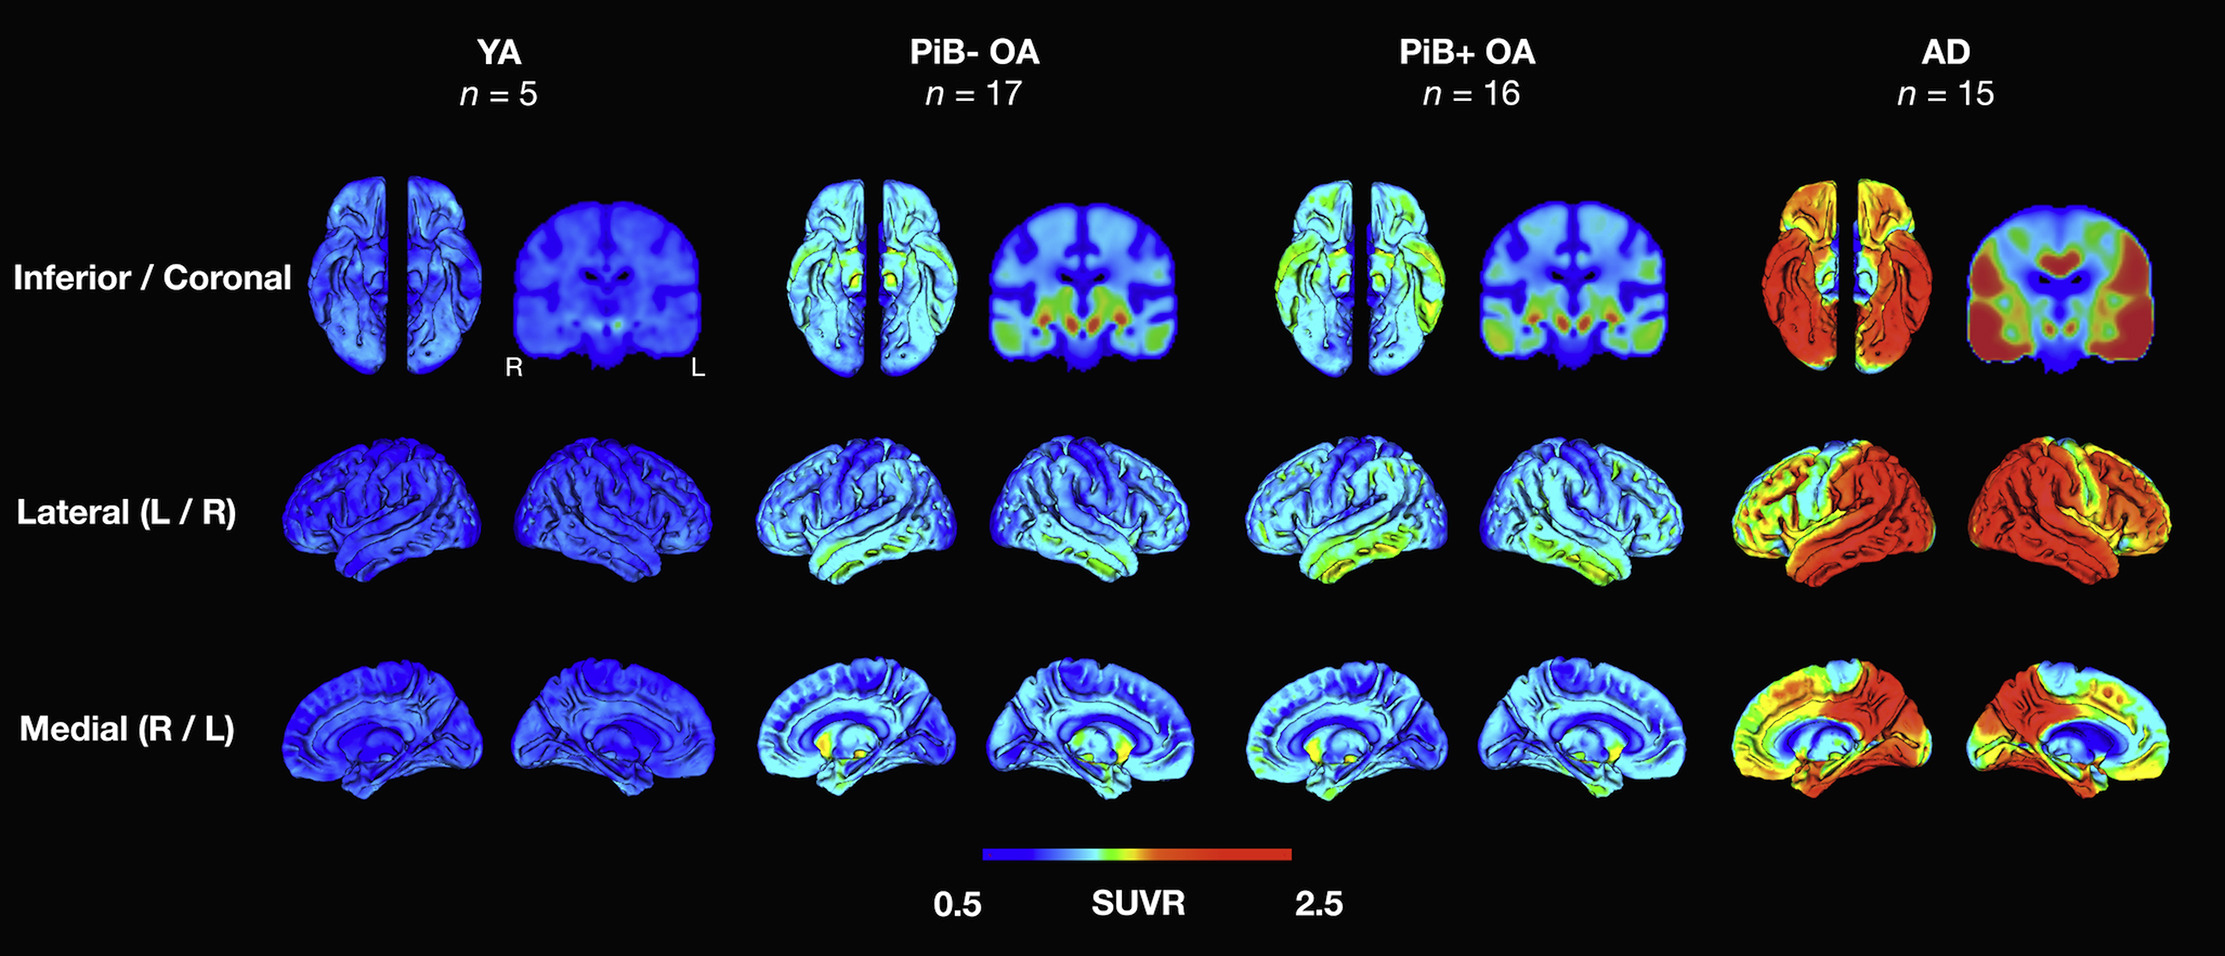
\includegraphics[width=\textwidth]{scholl-stages.jpeg}
    \centering
    \caption{\textbf{Stages of $\tau$-protein progression from SUVR.} 
    Figure adapted from \cite{SCHOLL2016971}, showing the mean \TP
    SUVR in a young adult population (YA), older adults (OA) with and without
    amyloid (determined by PiB PET), PiB- and PiB+, respectively, and subjects
    diagnosed with AD.}
    \label{fig:taustaging}
\end{figure}

In parallel with evidence toward the prion-like nature of \AB and \TP, AD
patients exhibit conserved patterns in the spread of these proteins through the
brain \cite{braak1991neuropathological, grothe2031, SCHOLL2016971,cho2016vivo}.
Typically, \AB begins globally in the neocortex and progresses subcortically.
Conversely and in a more pronounced fashion, whereas \TP displays more
incremental staging, starting from the entorhinal and spreading regions to
surrounding medial temporal structures, then the lateral temporal and then
finally into frontal and parietal cortices \cite{lowe2016,
SCHOLL2016971,Ossenkoppele2016, cho2016vivo}. The progression of atrophy is
correlated to the progression of toxic proteins, particularly with that of \TP
\cite{harrison2019longitudinal, xia2017association, cho2016vivo, jack2018nia,
pini2016}. The stereotypical patterns of toxic protein deposition and atrophy
provide a valuable bio-marker for the assessment AD pathology, particularly in
regions effected early in disease progression such as the hippocampus
\cite{echavarri2011atrophy, jack2011steps, eskildsen2015structural}.

\section{Imaging Alzheimer's Disease}\label{sec:1-imaging}

The ability to compare models and observations is crucial for determining their
utility. At present, observations are gathered through brain imaging,
namely PET studies and structural MRI (sMRI). There are a number of
publicly available data libraries containing such data specific to AD, most
notably the Alzheimer's Disease Neuroimaging Initiative (ADNI) and the Swedish
BioFINDER study. Additionally, there are a number of community standard software
libraries for the analysis of brain images. Particular software that are
utilised throughout the work presented here are FreeSurfer
\cite{fischl2012freesurfer} and FSL \cite{jenkinson2012fsl}. The combination of
publicly available data and analysis software has eased the burden on modellers
for finding and processing observational data.  

Since its inception, neuroimaging has proved a valuable tool for investigating
AD in humans. Without such methods, it would be near impossible to analyse
practically AD pathology in-vivo in human brains. The recent advent of \TP PET
tracers has allowed for such observations to be made
\cite{schwarz2016regional,xia201318f, marquie2015validating,
honer2018preclinical}. Two of the most popular radiotracers are the first
generation AV1451, used in ADNI \cite{landau2016flortaucipir}, and second
generation RO948 used in the second Swedish BioFINDER study (BF2)
\cite{ossenkoppele2021accuracy}. These tracers primarily bind to tau lesions
comprised of paired helical filaments, which allows for the quantification of
\TP related AD pathology \cite{smith2020head}. However, radiotracers also
exhibit off-target binding, attaching to molecules other than paired-helical
filaments of \TP and resulting in false signal. This can significantly limit the
utility of tracers in the affected brain regions. AV1451 signal exhibits
particularly strong contamination in the basal ganglia and choroid plexus
\cite{lowe2016autoradiographic,lemoine2018,choi2018off}. While these are not
areas that typically show particularly strong invasion in AD, the affect of
off-target binding interferers with signal in important surrounding areas,
namely the hippocampus \cite{johnson2016tau, lowe2016autoradiographic}. These
issues are partially circumvented with next generation tracers, such as RO498,
that show negligible binding in the choroid plexus and reduced binding the basal
ganglia \cite{smith2020head, kuwabara2018evaluation, wong2018characterization}. 

An example of how \TP PET can be used to monitor disease progression is shown in
\cref{fig:taustaging}, adapted from \cite{SCHOLL2016971}. Here, the authors use
a combination of an \AB PET tracer (PiB) and a \TP tracer (AV1451) to track
disease progression from young adults (YA), to older adults without \AB (PiB-
OA), older adults with \AB (PiB+ OA) and finally patients diagnosed with AD.
\cref{fig:taustaging} shows the mean \TP PET standardised uptake value ratio
(SUVR) in each of these groups. The figure demonstrates two important features
of \TP PET. First, \TP PET is able to capture the pronounced staging of \TP
through the brain during AD progression. Second, \TP staging observed through
PET differs from that observed through post-mortem histological analysis
\cite{braak1991neuropathological}, in particular through strong \TP signal
involvement in the occipital lobe. The differences in staging likely arise from
regional variations in tracer dynamics, such as uptake and binding affinity.
Tracer staging profiles have now been extensively validated \cite{lowe2016,
cho2016vivo, vogel2020spread, biel2021tau, vogel2021four}.

These data have been used extensively by modellers for parameter calibration and
validation \cite{vogel2020spread,schafer2020network,schafer2021bayesian}.
Similarly, studies using structural MRI have shown how atrophy progresses during
AD \cite{whitewell2010}, highlighting the relationship between atrophy and \TP,
but not \AB \cite{Ossenkoppele2016,SCHOLL2016971,lowe2016}. As yet, few studies,
have used structural MRI as observations to fit models, however, their relative
abundance compared to PET data make them a valuable resource for modelling,
especially if they can be usefully combined for multimodal inference
\cite{raj2012network,raj2015network,schafer2022correlating}. Overall,
neuroimaging has provided a wealth of knowledge and data that has advanced AD
research in its own right, and has also facilitated modelling studies probing
disease mechanism.

\section{Dynamical Models of AD}\label{sec:1-uncertainty}

Network models of neurodegeneration have been used extensively to study the
progression of toxic proteins during AD but come with a number of challenges,
some inherent with dynamical systems models and some particular to the modelling
domain, i.e. network neuroscience.  The basic mechanisms these models describe
are transport across axons and growth via an autocatalytic prion-like process.
The first model, describing only transport through axons, was provided by
\cite{raj2012network} and laid the foundation for other groups to expand on this
with more expressive models that describe growth
\cite{fornari2019prion,fornari2020spatially,weickenmeier2018multiphysics}.  
The general form of these models is a system of ordinary differential equations
on a graph: 
\begin{equation}\label{equ:general-system}
\odl{\mathbf{u}}{t} = \tns{f}(\tns{u},  t; \tns{p}, \tns{L}),
\end{equation}
where $\tns{f}$ is a vector valued function in time, with state vector $\tns{u}
\in \mathbb{R}^N$, additionally depending on parameters, $\tns{p} \in
\mathbb{R}^p$, and a $N \times N$ Laplacian matrix, $\tns{L}$, derived from a
graph used to define the domain of the system. Representing the system in this
way highlights the challenges present in the modelling process, since each
element of the system brings its own form of uncertainty that requires
quantification and rectification. 

First, there is uncertainty about the nature of the function $\tns{f}$,
principally due to our limited understanding of AD pathology. Several models
have been presented in the literature, including the simple network diffusion
model \cite{raj2012network,raj2015network}, the epidemic spreading model
\cite{vogel2020spread} and a host of reaction-diffusion equations
\cite{fornari2019prion,fornari2020spatially}. Each of these models imbue
different processes and assumptions into a model of AD pathology and at present
there is little evidence to choose one over another. Thus it is important to  be
able to identify which of these models is most appropriate given the available
data. There are numerous methods available for this, including a host of
information criteria, such as the Akaike information criteria, and more advanced
methods such as Bayesian leave-one-out cross validation
\cite{gelman2014understanding}.

\begin{figure}[t]
    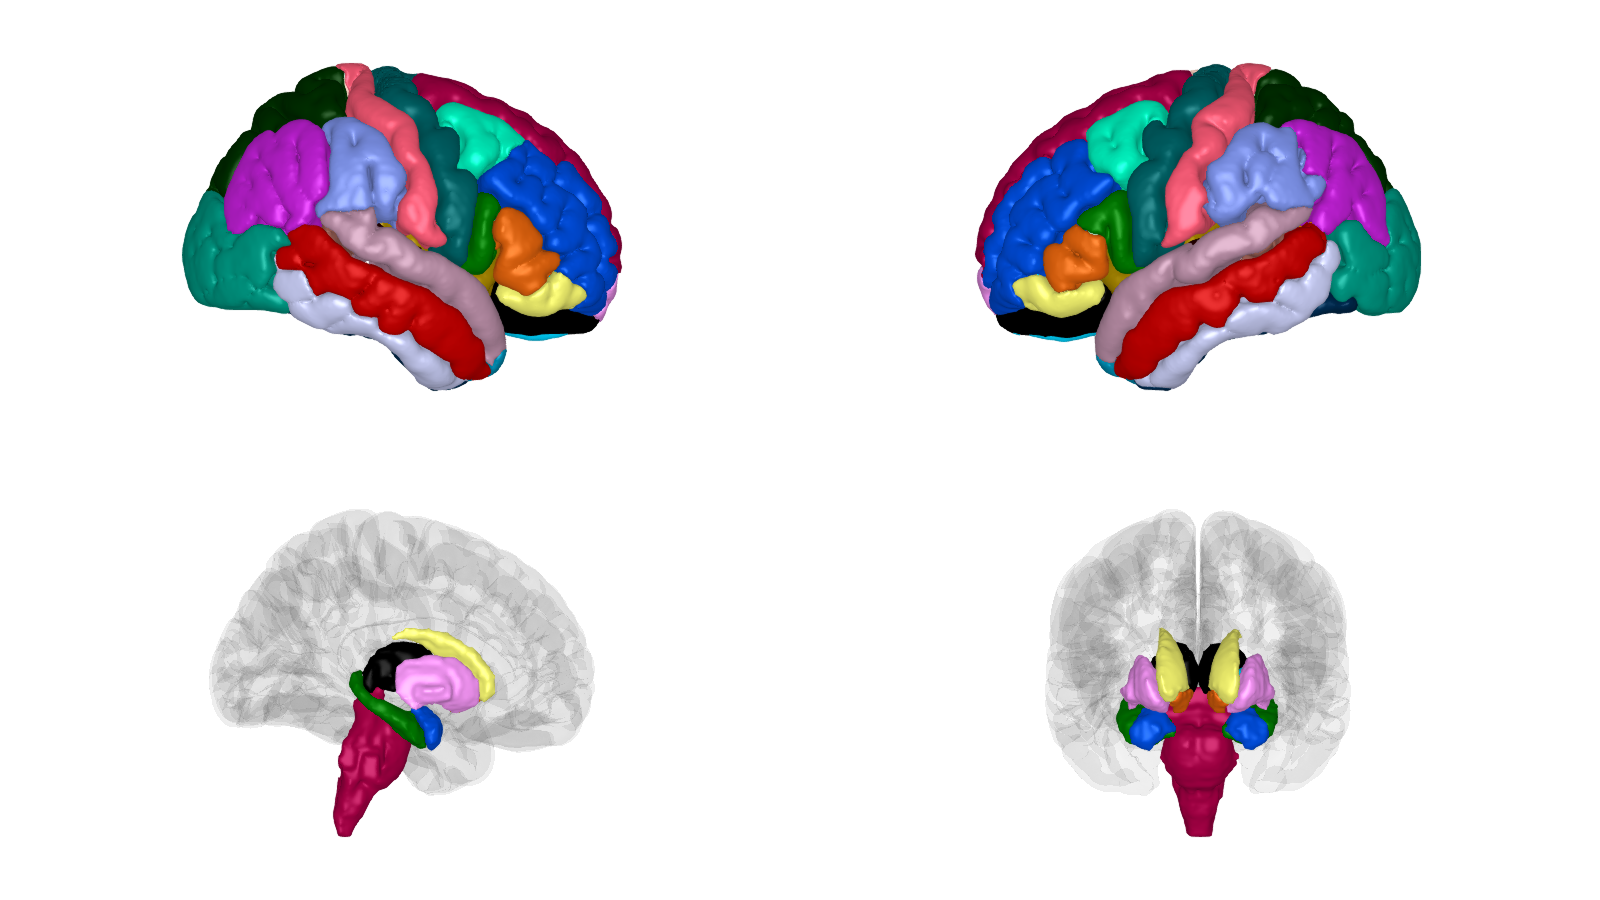
\includegraphics[width=15cm, height=9cm]{parcellation.png}
    \centering
    \caption{\textbf{The DKT parcellation}. The standard FreeSurfer DKT
    parcellation shown on a MNI brain. Top: 68 cortical regions for left and
    right hemispheres. Bottom: 15 subcortical regions, including the brainstem}
    \label{fig:parcellation}
\end{figure}

Second, there is considerable uncertainty associated with the graph used to
define the dynamical system. The graph not only defines the state vector,
$\tns{u}$, but the transport between its elements, and therefore its properties
can have a large effect on the dynamics of the system. The process of
generating a graph, referred to in network neuroscience as a connectome, can be
broadly separated into two processes: 1) parcellating the brain; 2) performing
tractography. Each of these two processes are active areas of research in
imaging neuroscience and there is no canonical choice for either, leading to
sources of uncertainty stemming from both. 

For the current work, we generate connectomes using the
Desikan-Killiany-Tourville (DKT) parcellation supplied as standard in the FreeSurfer
software package \cite{fischl2004automatically, klein2012101} and visualised in
\cref{fig:parcellation}. However, there are many alternative parcellation
choices, each of which characterise different features of brain, e.g. anatomy,
functional connectivity, size of regions, gyrification, among others
\cite{lawrence2021standardizing, moghimi2021review}. It is not yet known whether
some parcellations are better suited than others for marco-scale connectome
modelling.  

Tractography is a process of reconstructing the neuronal connections between
brain regions from diffusion weighted MRI imaging (dMRI). There are two broad
families of tractography methods, deterministic and probabilistic. Both methods
seek to simulate streamlines, synthetic fibers that follow the estimated fiber
orientation at each voxel. Deterministic tractography follows the trajectory of
streamlines using fixed fiber orientations at each voxel, whereas probabilistic
tractography uses a distribution of fiber orientations at each voxel to account
for uncertainty in possible streamline direction \cite{sarwar2019mapping}. The
output of tractography is an adjacency matrix that defines a graph representing
connections between regions of a given parcellation. Connectomes generated using
different procedures are shown in \cref{fig:connectome}.
\cref{fig:connectome-diffusive-fsl} shows a connectome generated with
probabilistic tractography using FSL, while \cref{fig:connectome-diffusive-pit}
shows one generated using deterministic tractography
\cite{szalkai2017parameterizable,kerepesi2017braingraph}, distributed by the PIT
group through \url{www.braingraph.org}. Differences in network topology, such as
those shown between
\cref{fig:connectome-diffusive-fsl,fig:connectome-diffusive-pit}, can have
significant effects on the dynamics exhibited on those networks
\cite{putra2021braiding}. Together with the lack of consensus about how to
generate connectomes, this creates a large source of uncertainty in the
modelling process. In this work, we use connectomes generated using the default
pipelines in FSL, which have been extensively validated
\cite{behrens2003characterization,behrens2007probabilistic,warrington2020xtract},
and data from the HCP.
\begin{figure}[t]
    \centering
    \begin{subfigure}[b]{0.8\textwidth}
        \centering
        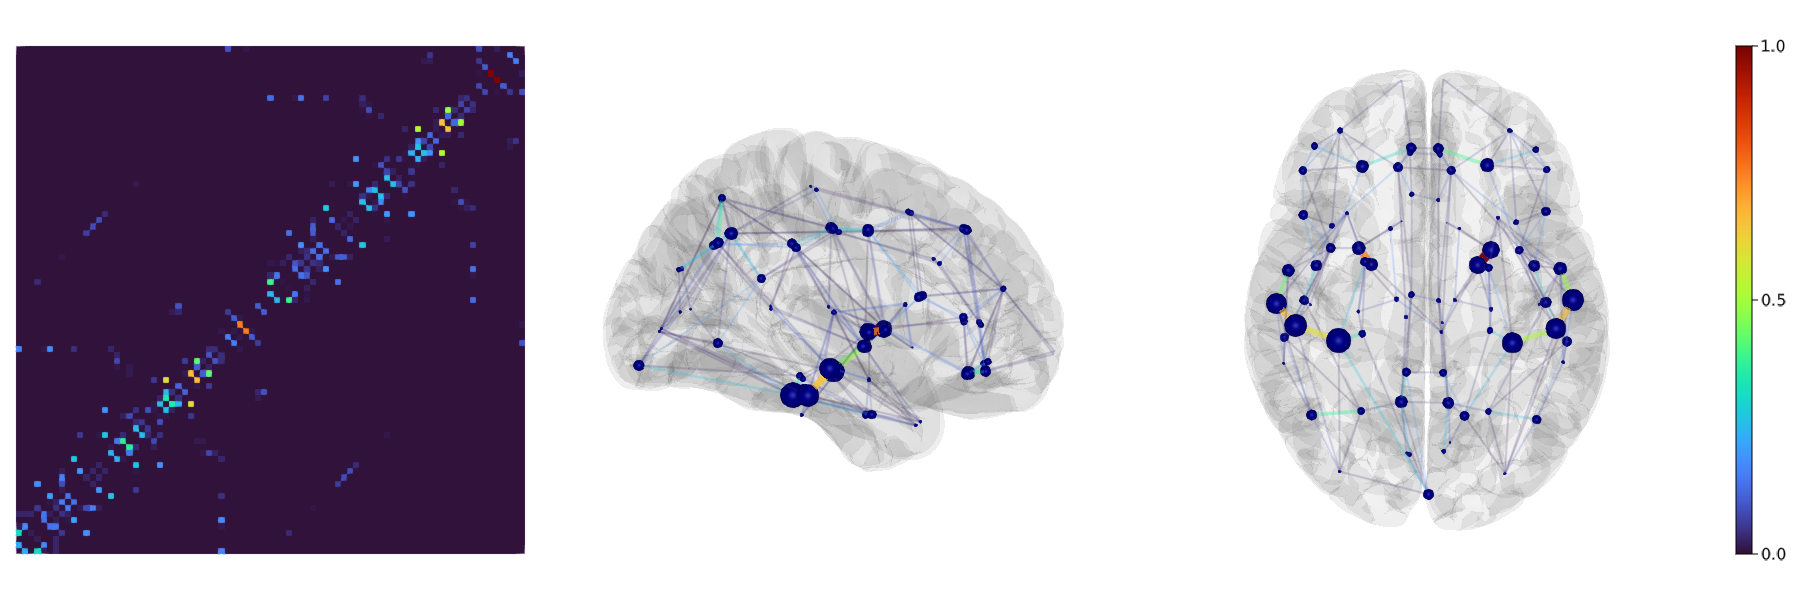
\includegraphics[width=\textwidth]{connectomes/connectome-diffusive.png}
        \caption{Probabilistic connectome with diffusive weights}
        \label{fig:connectome-diffusive-fsl}
    \end{subfigure}
    \begin{subfigure}[b]{0.8\textwidth}
        \centering
        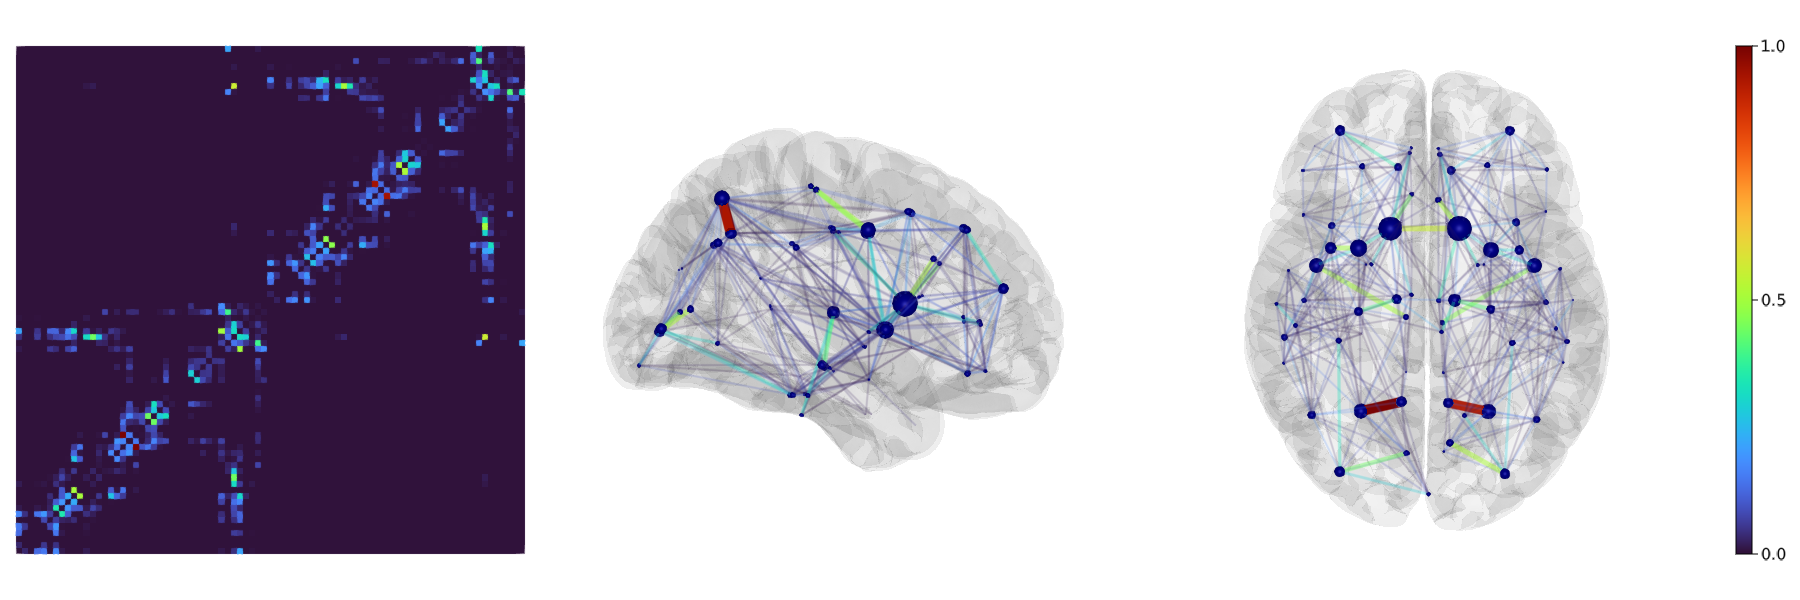
\includegraphics[width=\textwidth]{connectomes/connectome-pit.png}
        \caption{Deterministic connectome with diffusive weights}
        \label{fig:connectome-diffusive-pit}
    \end{subfigure}
    \caption{\textbf{Connectomes made with different tractography procedures}.\\
    Both connectomes are made using the DKT atlas to define regions of interest.
    Left: Shown are weighted adjacency matrices normalised to the maximum
    values. Right: networks visualised on the brain; edges coloured by weight
    and and vertices sized by degree. Networks have been filtered using a naive
    threshold of 0.01. \textbf{(a)} Made using FSL probabilistic tractography
    \cite{behrens2003characterization,behrens2007probabilistic}. \textbf{(b)}
    Made using MRtrix deterministic tractography and distributed by the PIT
    group through \url{www.braingraph.org} \cite{kerepesi2017braingraph}.}
       \label{fig:connectome}
\end{figure}

Third, there is parametric uncertainty associated with the parameter vector,
$\mathbf{p}$. For any given dynamical system, variations in parameters can lead
to different model behaviours. In general, it is difficult to infer from
observations alone the parameters of the dynamical system, a problem that is
made more challenging in the presence of observation noise. Popular methods for
inferring parameter values include least squares regression, maximum likelihood
estimation and maximum a-posteriori estimation and have been used in the network
neurodegeneration literature for model validation
\cite{raj2012network,raj2015network,vogel2020spread}. However, forr ill-posed
problems with sparse and noisy observations, and where data are assumed to be
generated from a non-linear process, these methods are unsuitable since they do
not account for potentially significant parametric uncertainty. The effect of
parameter variations on the dynamics of models for neurodegeneration has been
shown in \cite{putra2021braiding}. We have recently presented work which has
incorporated Bayesian analysis into the validation pipeline, which allows for
the quantification of uncertainty
\cite{schafer2020network,schafer2021bayesian,schafer2022correlating}. The
results highlight that there can be considerable variation in parameters between
individuals and groups for a given set of observations. A framework for handling
sources of uncertainty has been the focus of this project thus far and will be
discussed in \cref{chp:2}, with applications in \cref{chp:3}. 

\section{Research Aims and Report Overview}

\subsection{Research Aims}
My aim is to establish a mathematical and software framework for validating
dynamical models of AD with human neuroimaging data. My objectives are to: 

\begin{enumerate} 
    \item Develop a unified mathematical and software pipeline that
    simplifies dynamical modelling of AD and inference with patient data. 
    \item Apply this framework to answer specific questions about AD
    progression.
\end{enumerate}

\subsection{Report Overview}
The remainder of the report is organised as follows. In \cref{chp:2}, I
will discuss the mathematical models that are used throughout this report. I
will also overview the general problem of using Bayesian inference for
time-series problems. In \cref{chp:3}, I will present recent work on the
application of dynamical systems, generative modelling and Bayesian inference to
problems in neurodegeneration. In \cref{chp:4}, I offer some concluding
remarks and a proposal for future work.
Parts of this report are taken from the following publications and highlighted
accordingly: 
\begin{itemize}
    \item \fullcite{schafer2022correlating} \textbf{Joint first author.}
    \item \fullcite{schafer2021predicting} \textbf{Joint first author.}
    \item \fullcite{putra2021braiding}
    \item \fullcite{thompson2020}
\end{itemize}
The results presented in \cref{chp:3} reflects my most recent work 
and is currently being prepared for publication.


\chapter{Mathematical Models of Alzheimer's Disease}
\label{chp:2}
Mathematical modelling of AD has becoming a fertile research programme in recent
years, producing models that describe disease mechanisms and making valuable
predictions about patient trajectories \cite{raj2015network, fornari2019prion,
thompson2020, schafer2022correlating}. In particular, network models of
neurodegeneration have become increasingly popular due to the desirable balance
of complexity and explanatory power. Here, I will describe the basis for network
mathematical models of AD and some of the models used in the literature and
throughout this report.

Typically, mathematical models of neurodegeneration have focussed on modelling
the spread, accumulation and aggregation of toxic protein species, \TP and \AB.
While there have been numerous contributions focussing on continuum dynamics
\cite{weickenmeier2018multiphysics,fornari2020spatially}, as well as
probabilistic network models \cite{vogel2020spread}, I will here focus on
dynamical models on networks. More specifically, I will focus on modelling of
\TP, since it displays richer spatiotemporal dynamics that are more tightly
coupled with atrophy and symptom onset, as discussed in \cref{sec:1-bio-ad}. The
use of such network models is motivated by experimental results demonstrating
that \TP preferentially travels through axonal fibres \cite{liu2012trans,
de2012propagation, devos2018synaptic}.  
An additional benefit is that solutions to ordinary differential equations
(ODEs) on graphs are computationally less expensive to obtain than their partial
differential equation counterparts. As mentioned in
\cref{sec:1-uncertainty}, network models of AD protein pathology should aim to
describe at least transport across axons and growth via an autocatalytic process
akin to prion-like templating.

\section{Transport and the Graph Laplacian}
\label{sec:transport}
As highlighted in \cref{sec:1-uncertainty} the graph Laplacian is the central
object used to describe transport along axonal fibres. The topology of axonal
pathways can be obtained through the analysis of diffusion weighted MRI data,
such as those available from the Human Connectome Project. The output of
this analysis is a graph $G = (V, E)$, where $V$ is the enumeration of vertices
in the graph, $v_1, v_2, . . . v_n$ and $E$ the edges between them. The
transport of protein concentration between regions of the brains, vertices $V$,
can be effectively modelled using the graph Laplacian, given by:
\begin{equation}\label{eqn:laplacian_matrix}
    \mathbf{L} = \mathbf{D} - \mathbf{A},
\end{equation}
where $\tns{A}$ is an adjacency matrix encoding the connectivity between 
regions.
\begin{equation}\label{eqn:adjacency_matrix}
A_{ij} = \left\{\begin{array}{cl} 1 & \text{if an edge connects } v_i \text{ to } v_j\\ 0 
                            & \text{otherwise}\end{array}\right.,
\end{equation}
and $\tns{D}$ is the degree matrix, containing the total number of edges associated with a given vertex, 
\begin{equation}\label{eqn:degree_matrix}
D_{ij} = \delta_{ij} \sum_{j=1}^{N} A_{ij}.
\end{equation}

We can include more information about the connectivity of the brain regions by
weighting the adjacency matrix by the number and length of streamlines estimated
between regions from tractography. The choice of weighting has been extensively
discussed in \cite{putra2021braiding}. In this work, we describe transport of
toxic protein as diffusion across the brain network. The appropriate edge
weighting to describe such a process is: 
\begin{equation}
    \label{eqn:edge-weighting}
    A_{ij} = \frac{n_{ij}}{l_{ij}^{2}}
\end{equation}
where $A_{ij}$ is the edge connecting $v_i$ and $v_j$, $n_{ij}$ is the number of 
streamlines between $v_i$ and $v_j$, and $l_{ij}$ is the average length of those 
streamlines.

Using the graph Laplacian, the transport of proteins by diffusion on a graph is
given by the network heat equation: 
\begin{equation}\label{eqn:ndmodel}
    \odl{\tns{p}}{t} = -\rho \tns{L}\tns{p},
\end{equation}
where $\mathbf{p} \in \mathbb{R}^{N}$ is the protein concentration at each node
in the brain network, $\rho \in \mathbb{R}$ is the diffusion coefficient, and
$\mathbf{L} \in \mathbb{R}^{N \times N}$ is the graph Laplacian with weights
given by \cref{eqn:edge-weighting}. This model has been analysed against
data using regression studies \cite{raj2012network,raj2015network} and Bayesian
inference \cite{schafer2020network}. However, there is a wealth of evidence to
suggest that this model is not an accurate description of the prion-like process
underlying AD, since it does not account for growth coming from the prion-like
templating process \cite{jucker2013self,fornari2019prion}.

\section{Protein Proliferation}
\label{sec:growth}
\subsection{The Heterodimer Model}
To augment the network heat equation with appropriate production 
and clearance term, consider the kinetic diagram shown in \cref{fig:hxdkinetics}, 
describing Pruisner's model of prion-like propagation through templating 
\cite{prusiner1991, prusiner1998}. 
\begin{figure}[h]
    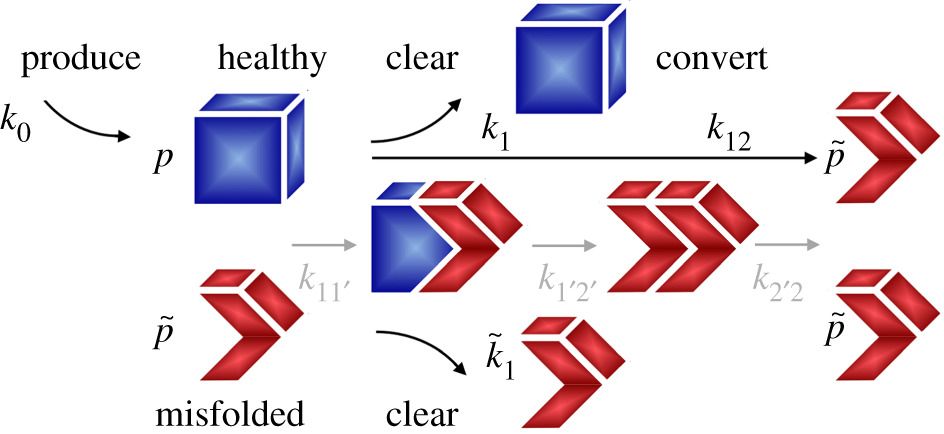
\includegraphics[width=8cm]{heterodimerkinetics.png}
    \centering
    \caption{\textbf{Reaction kinetics of the heterodimer model.} Adapted from \cite{fornari2019prion}.}
    \label{fig:hxdkinetics}
\end{figure}
There is a healthy protein concentration, $p$, and toxic protein species,
$\hat{p}$. The toxic protein binds the healthy protein with rate $k_{11'}$ and
induces a conformational change into the healthy protein, turning it into a
toxic protein at rate $k_{1'2'}$, before separating into two toxic monomers with
rate $k_{2'2}$. This is collectively summarised as rate $k_{12}$. Both healthy
and toxic protein species are cleared with a natural clearance rate of $k_1$ and
$\hat{k}_1$, respectively. With the addition of transport between regions, this
can be expressed as a pair of coupled ODEs:
\begin{subequations}
    \label{eqn:network-heterodimer}
    \begin{alignat}{3}
        \odl{p_i}{t} &=  -\rho\sum\limits_{j=1}^{N}\mathcal{L}_{ij}p_j +  k_0 &&- k_1 p_i - k_{12}p_i \hat{p}_i, 
        \label{eqn:network-heterodimer:healthy}\\
        \odl{\hat{p}_i}{t} &= -\rho\sum\limits_{j=1}^{N}\mathcal{L}_{ij}\hat{p}_j &&- \hat{k}_1 \hat{p}_i + k_{12}p_i\hat{p}_i. 
        \label{eqn:network-heterodimer:toxic}
    \end{alignat}
\end{subequations}
where $p_i \in \mathbb{R}$ and $\hat{p}_i \in \mathbb{R}$ for $i = 1 \hdots N$
are healthy and toxic protein concentration for $N$ nodes, respectively, $\rho$
is the diffusion coefficient and $\mathcal{L}_{ij}$ is the $ij$-th element of
the graph Laplacian, $\mathbf{L} \in \mathbb{R}^{N \times N}$. The combination
of Pruisner's kinetic model with the network diffusion equation provides a
mechanistic description of AD in terms of protein transport and growth
\cite{fornari2019prion}.

The physical insight obtained comes at the cost of an increased number of
parameters. For simulation purposes, this does not pose any issues, however, as
we will see in later sections, it will prove problematic for inference. Given
the temporal sparsity of data, it will be challenging to identify the parameters 
of complex models. Using a few assumptions, we can reduce the model to one 
with fewer parameters and similar global behaviour. 

\subsection{Reduction to FKPP model}
\label{sec:model-reduction-fkpp}
To simplify the heterodimer model \cref{eqn:network-heterodimer}, we can
linearise around a healthy state. First, we assume a healthy, homogenous state
with $\tilde{p}_i \ll p_i$, implying $\nicefrac{\mathrm{d}p_i}{\mathrm{d}t} = 0$ and
$-\lap{p_j} = 0$ for $i = 1 \hdots N$. Then, using 
\cref{eqn:network-heterodimer:healthy}, we can write $p$ as a function of
$\tilde{p}$
\begin{align*}
    0 &= k_0 - k_1 p_i - k_{12}p_i \hat{p}_i \\ 
    p_i(\tilde{p_i}) &= \frac{k_0}{k_1 + k_{12}\tilde{p}_i}.
\end{align*}
Linearising around $\tilde{p} = 0$, we have 
\[
    p_i(\tilde{p}_i) \approx \frac{k_0}{k_1}\left(1-\frac{k_{12}}{k_1}\tilde{p}_i\right).    
\]
Substituting this expression for $p$ into
\cref{eqn:network-heterodimer:toxic} we obtain, 

\begin{equation}\label{eqn:fkpp-goriely}
    \odl{\tilde{p}_i}{t} = - \rho \lap{\tilde{p}_j}  
                        + \beta \tilde{p} 
                         -\alpha\tilde{p}^2,
\end{equation}
where 
\begin{equation}
    \beta = \frac{k_0}{k_1}k_{12} - \tilde{k}_{1} 
    \qquad \text{and} \qquad 
    \alpha = \frac{k_0 k_{12}^2}{k_1^2}.
\end{equation}
To derive the canonical FKPP model, we make a change of variables
$\tilde{p} = c \beta\alpha^{-1}$, giving: 

\begin{equation}
    \label{eqn:fkpp-global}
    \odl{c_i}{t} = - \rho \lap{c_j} + \beta c_i \left( 1 - c_i \right)     
\end{equation}

The simulated dynamics of the FKPP model, \cref{eqn:fkpp-global}, are shown in
\cref{fig:fkpp-global}. The simulation showed has \TP seed of 50\% concentration
in the bilateral entorhinal cortex, with $\rho = 0.1$ and $\alpha = 1.2$. These
are synthetic parameters to used to illustrate the dynamics in a growth
dominated regime, $\rho \ll \alpha$. During the early stages of AD, the staging
of \TP across the connectome shares qualitative similarity with observed staging
in AD patients. However, there are some notable deficiencies that may prevent
the accurate prediction of patient disease from \TP PET observations. Notably,
the model in \cref{eqn:fkpp-global} does not account for regional variations in
tracer dynamics such as off-target binding, non-specific binding, tracer uptake
and binding-affinity. These factors are responsible for the heterogeneous SUVR
values observed in healthy individuals and and contribute to the distribution of
\TP tracer in end-stage AD subjects, as discussed in \cref{sec:1-imaging} and 
shown in \cref{fig:taustaging}. To address these issues, we next seek to
derive a model of \TP dynamics that incorporates these characteristics, whilst
still maintaining the reduced complexity that permits inference with patient
data.

\begin{figure}[H]
    \centering
    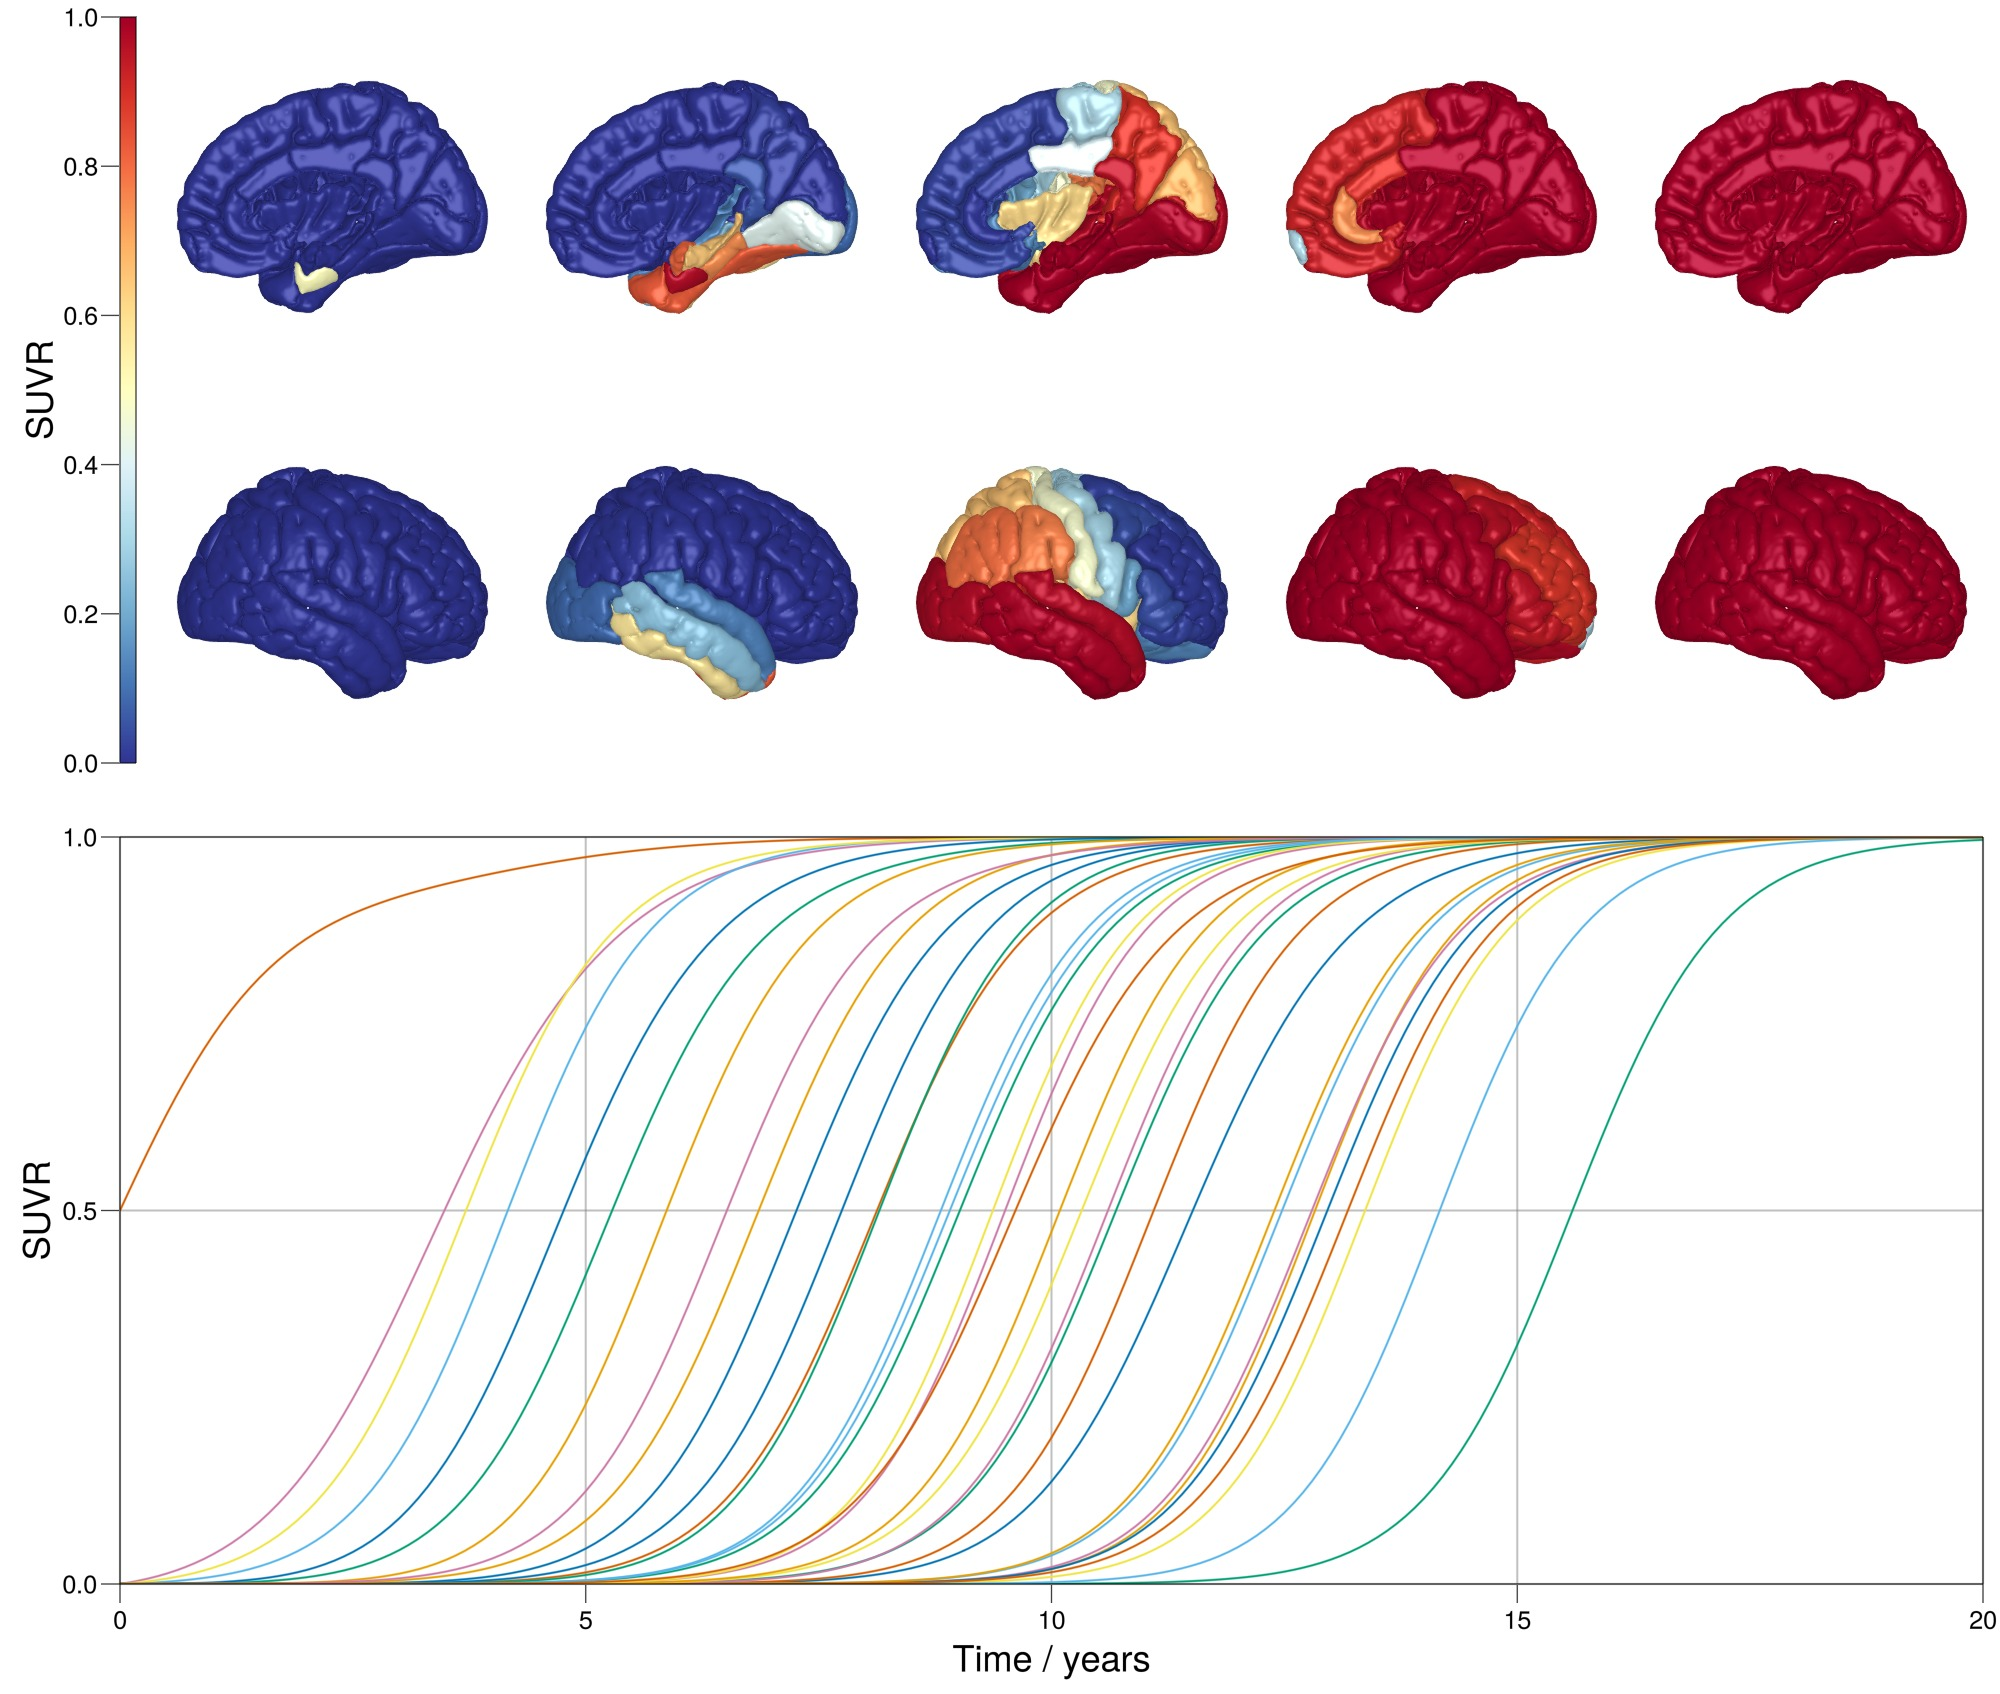
\includegraphics[width=0.9\textwidth]{local-fkpp/models/global-fkpp.jpeg}
    \caption{\textbf{Simulation from the global FKPP model}. \cref{eqn:fkpp-local}, 
    with bilateral seeding in the entorhinal cortex of 50 percent concentration, 
    $\rho = 0.1$ and $\alpha = 1.2$.}
    \label{fig:fkpp-global}
\end{figure}

\subsection{Local model of \TP pathology}
To derive a model that incorporates regional variations in tracer dynamics we
first follow the same steps to derive \cref{eqn:fkpp-goriely} from
\cref{eqn:network-heterodimer}.  We then make a change of variables to $s_i =
\tilde{p}_i + s_{0,i}$  to accommodate the potentially non-zero healthy baseline
level of observed \TP PET signal. Incorporating this change of variables, we
have: 
\begin{equation}\label{eqn:fkpp-suvr}
    \odl{s_i}{t} = - \rho \lap{\sso{j}}  
                        + \beta \sso{i} 
                         -\alpha \sso{i}^2,
\end{equation}
\[
    \beta = \frac{k_0}{k_1}k_{12} - \tilde{k}_{1} 
    \qquad
    \alpha = \frac{k_0 k_{12}^2}{k_1^2}.
\]
To determine regional carrying capacities, we again assume a healthy, homogenous
state, therefore: 
\begin{align}
    0 &= \beta \sso{i} - \alpha \sso{i}^2 \\
      &=\alpha\sso{i}\left(\beta \alpha^{-1} - \sso{i}\right).
    \label{eqn:static-fkpp}
\end{align}
Then, either $s_i = s_{0,i}$, at the minimum, or $s_i$ reaches 
its maximum when $s_i = \beta\alpha^{-1} + s_{0,i}$, which we define as
a new variable $s_{\infty,i}$, the carrying capacity. Therefore, we can rewrite
\cref{eqn:static-fkpp} as

\begin{equation}
    0 = \alpha \sso{i}\left[ \ssi{i} - \sso{i} \right].    
    \label{eqn:homogenous-local-fkpp}
\end{equation}

However, note that $s_{\infty,i} = \beta\alpha^{-1} + s_{0,i}$ implies
that the carrying capacity varies regionally only as a function of baseline
values, $s_{0,i}.$ The simplest assumption we can make to reflect regionally
varying carrying capacities, given the heterodimer model
\cref{eqn:network-heterodimer}, is to introduce a regionally varying clearance
rate of toxic protein, $\tilde{k}_1 \rightarrow \tilde{k}_{1,i}$, since it
appears only in our in carrying capacity through $\beta$ but not the uniform
growth rate $\alpha$. Therefore, the new definition for our carrying capacity is
$s_{\infty,i} = \beta_i\alpha^{-1} + s_{0,i}$ and our final model is
\begin{equation}\label{eqn:fkpp-local}
    \odl{s_i}{t} = - \rho \lap{\sso{j}}  
    + \alpha \sso{i} \left[\ssi{i} - \sso{i} \right],
\end{equation}
which defines a generative model of \TP SUVR, grounded upon a dynamical model of
\TP that accounts for regional variations in baseline values, $s_{0,i}$ and
carrying capacities $s_{\infty,i}$.


\subsection{Estimating Population Averaged Regional Parameters}
\label{sec:regionalparams}

\cref{eqn:fkpp-local} provides are a more realistic description of the 
observed \TP SUVR load in patients, however, it adds two parameter vectors, 
$\mathbf{p_0} \in \mathbb{R}^N$ and $\mathbf{p_\infty} \in \mathbb{R}^N$, for 
$N$ nodes in the brain network, therefore increasing model complexity and making 
it less practically identifiable. In this section, we provide a method
for estimating these parameters from data, allowing us to fix them ahead of
inference with individual subjects in \cref{sec:inference}. 

The approach used here extends the methods outlined in \cite{vogel2020spread}, 
in which Gaussian mixture models are used to estimate the 
probability of \TP infection. We fit a two 
component Gaussian mixture model to population level data of regional SUVR. 
For regions in which a reliable measure of \TP SUVR can be obtained, we expect 
to see two separable distributions, with one distribution capturing the 
expected, or healthy, \TP load in a given region, and one approximating the 
pathological \TP load. An example of this is given in \cref{fig:gmm-lit}, 
showing the SUVR values across the population for the inferior temporal lobe. 
In regions with a high degree of off-target binding, it is 
not possible to obtain a reliable measurement of \TP and thus making them 
difficult to model. An example of this 
can be seen in \cref{fig:gmm-lp}, showing a two component Gaussian 
mixture model fitted to the left putamen, a region known to display a high 
degree of off-target binding \cite{choi2018off}. These features associated wtih 
off-target binding are present throughout the subcortex, with exceptions in the 
hippocampi and amagydalae \cite{choi2018off, vogel2020spread}. To prevent
contamination with modelling results, we exclude these regions from our
connectome based models.

Using the remaining regions, $N = 72$, we estimate \p0 as the mean of 
the distributions describing describing healthy uptake. To approximate the 
carrying capacity, \pI, we use the 99-th percentile of the 
distributions describing pathological \TP burden. The derived baseline 
values and carrying capacities are visualised on the cortex in 
\cref{fig:baseline-capacities,fig:carrying-capacities}, respectively.
The cortex wide characteristics in baseline values, \p0 and carrying capacities,
\pI, are summarised in \cref{table:regionalparams}. The values of \p0 have
no important distinguishing features, with low variance around the mean. As
expected, the values of \pI are all higher than those of \p0. Additionally,
there is substantially more spread in the values of \pI across brain regions,
showing that carrying capacities are not uniform but rather have important
variations. These differences are more readily discerned from
\cref{fig:carrying-capacities}, in which it can be seen that the temporal,
occipital and lateral frontal regions have particularly high SUVR ranges. As
expected, the carrying capacities are consistent with in-vivo \TP staging and
longitudinal \TP PET neuroimaging studies (see \cref{fig:taustaging}) 
\cite{SCHOLL2016971,lowe2016, cho2016vivo}.

\begin{table}[h]
        \centering
        \begin{tabular}{lrrrr}
          \hline\textbf{Parameter} & \textbf{mean} & \textbf{std} & \textbf{min} & \textbf{max} \\\hline
          \p0 & 1.1108 & 0.0609 & 0.9818 & 1.2384 \\
          \pI & 2.4177 & 0.3773 & 1.9027 & 3.3321 \\\hline
        \end{tabular}
        \caption{Table of fixed parameters}
        \label{table:regionalparams}
\end{table}

\begin{figure}[H]
    \centering
    \begin{subfigure}{0.45\textwidth}
        \centering
        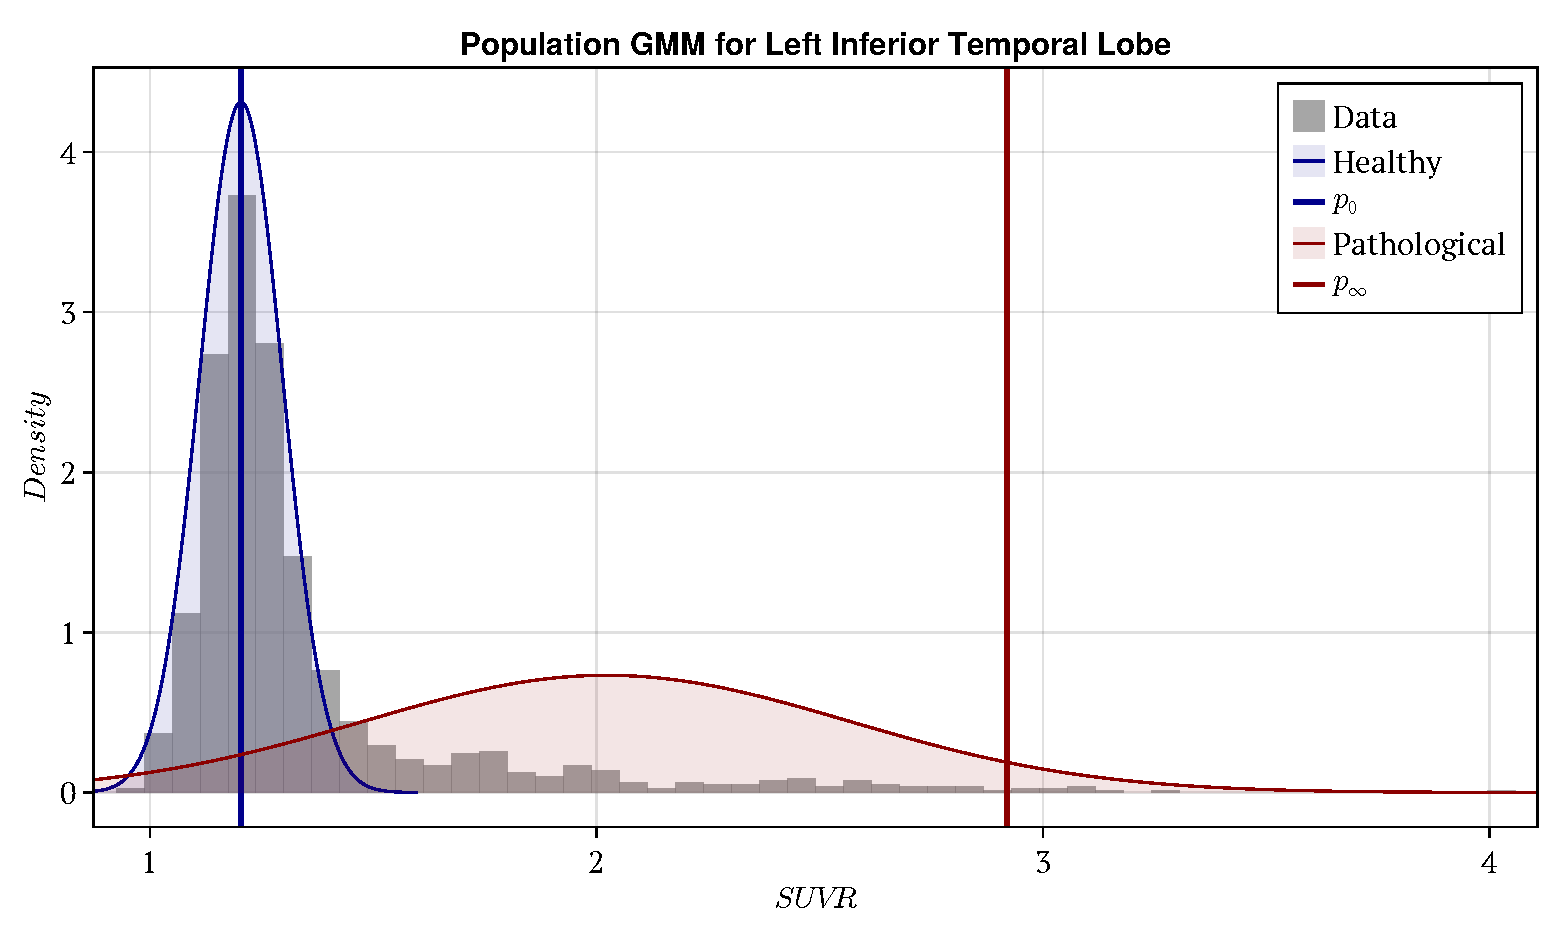
\includegraphics[width=\textwidth]{local-fkpp/models/gmm-lIT.pdf}
        \caption{GMM inferior temporal}
        \label{fig:gmm-lit}
    \end{subfigure}
    \begin{subfigure}{0.45\textwidth}
        \centering
        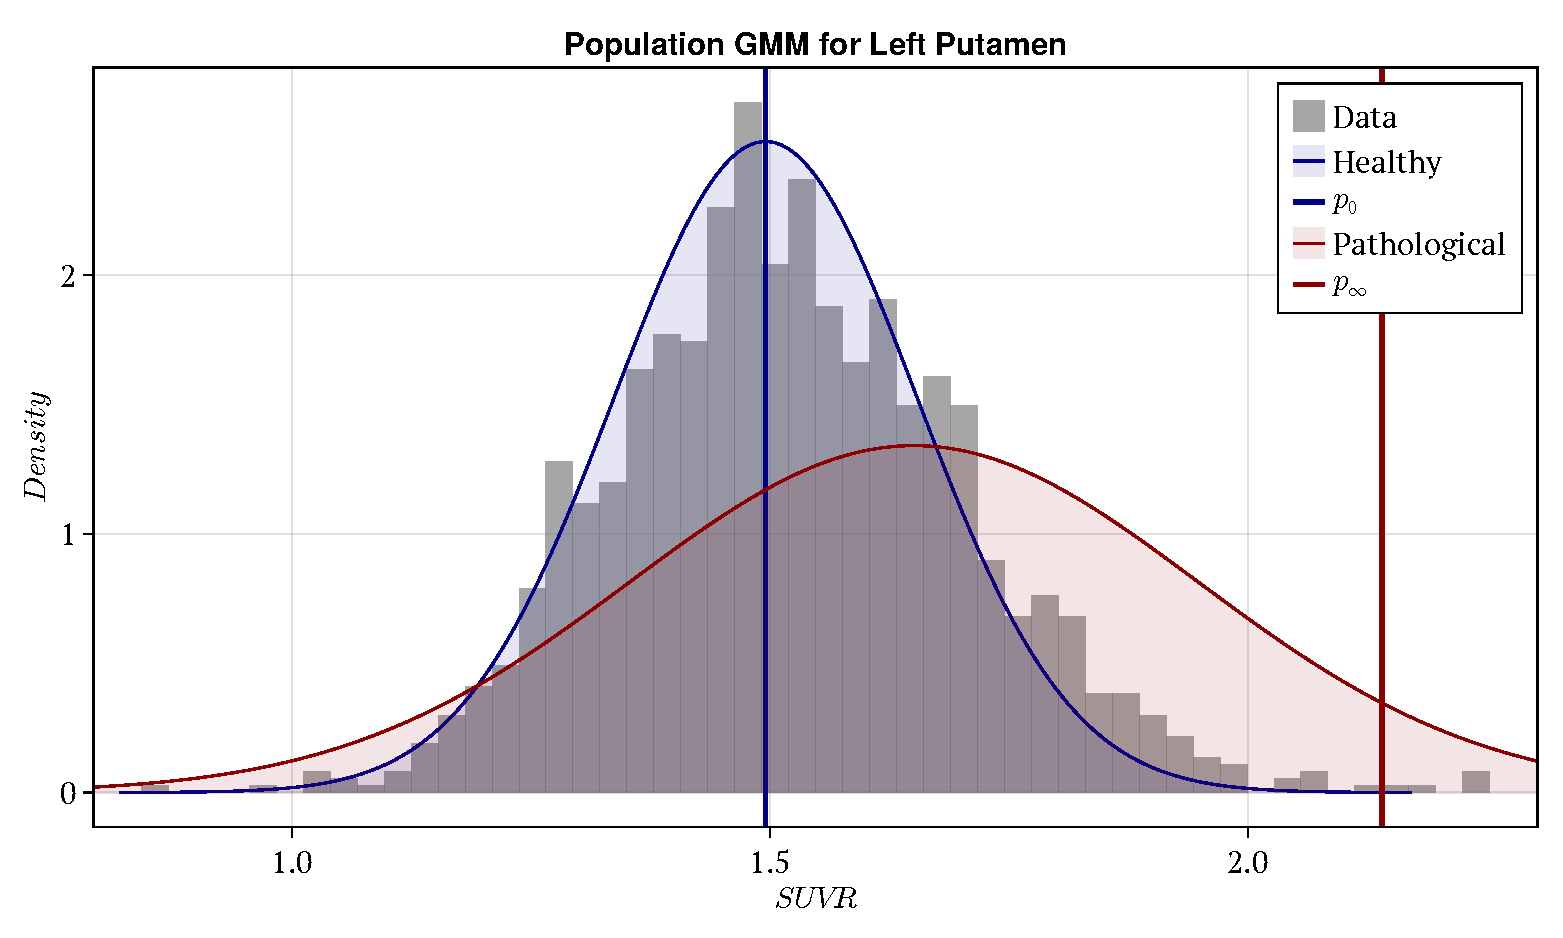
\includegraphics[width=\textwidth]{local-fkpp/models/gmm-lPutamen.pdf}
        \caption{GMM putamen}
        \label{fig:gmm-lp}
    \end{subfigure}
    
    \begin{subfigure}{0.95\textwidth}
        \centering
        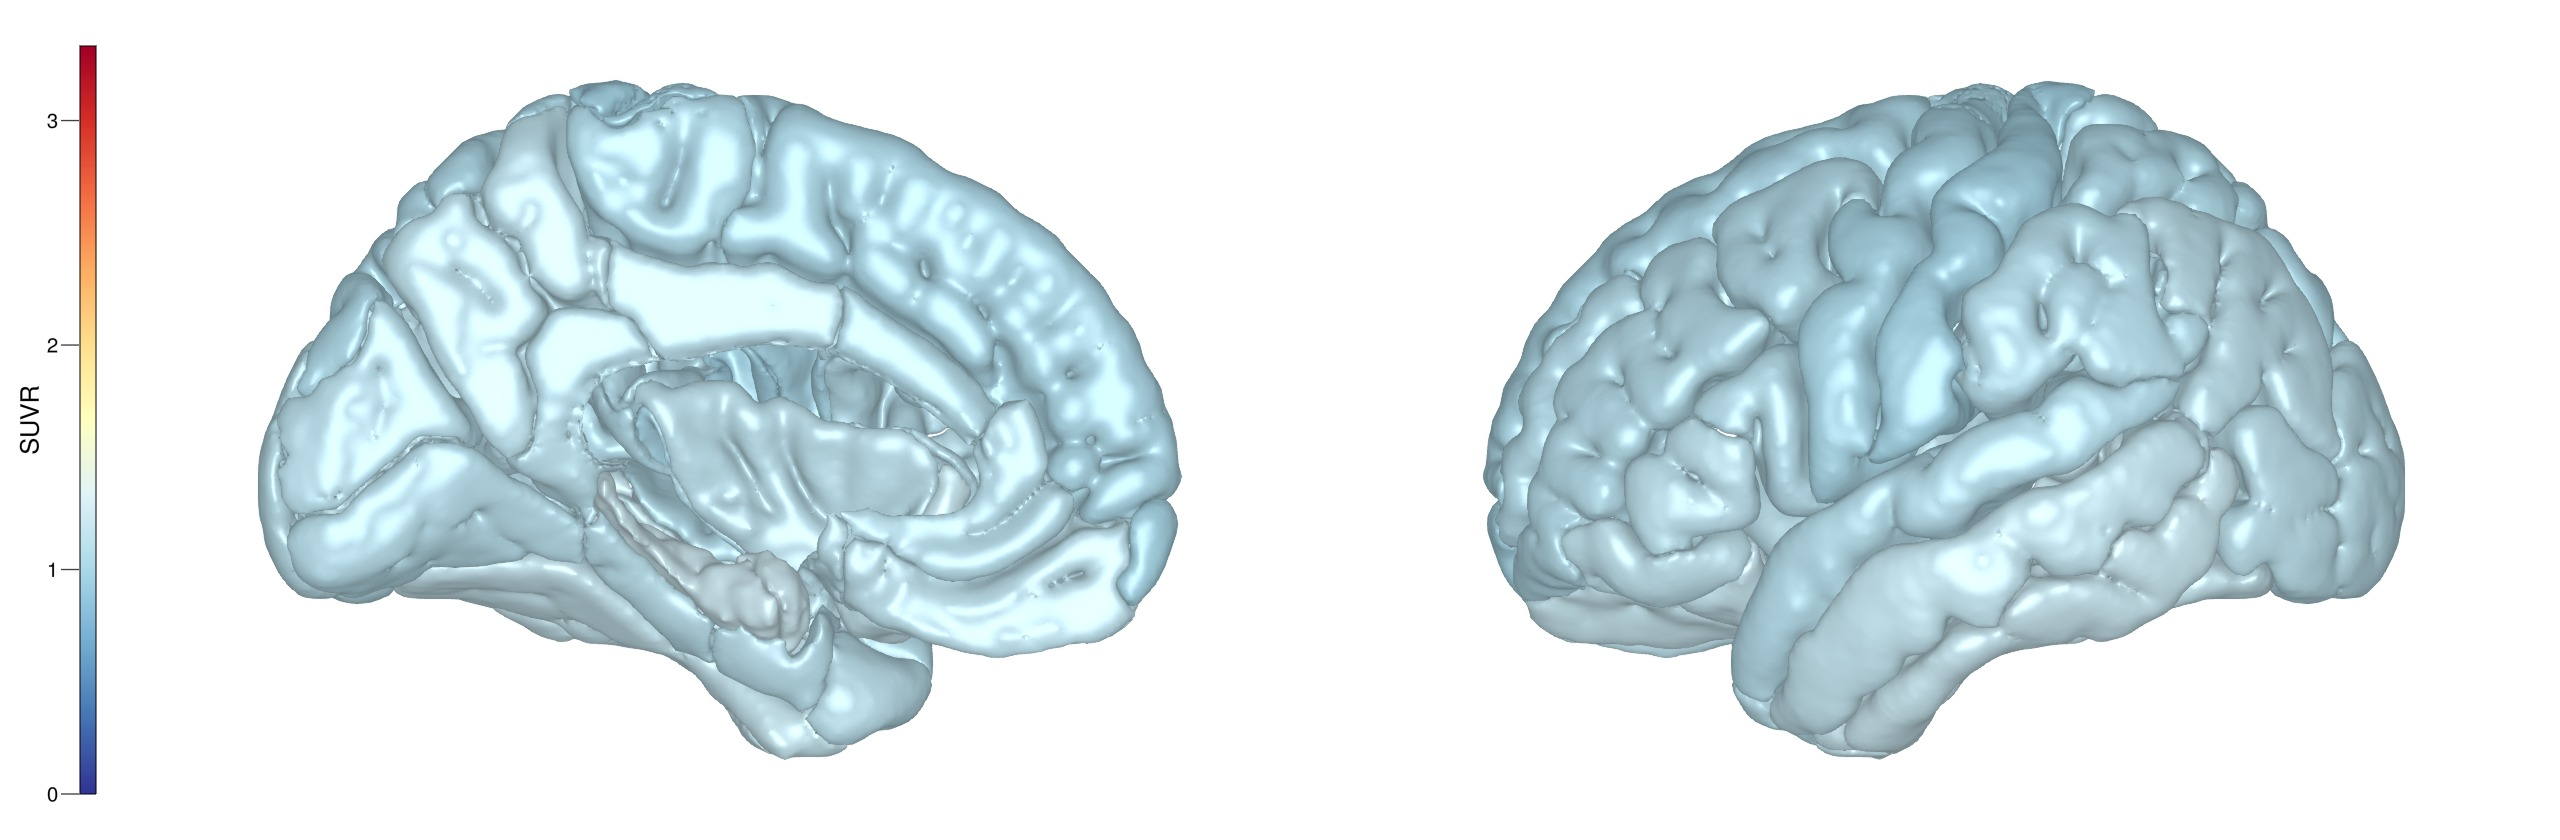
\includegraphics[width=\textwidth]{local-fkpp/models/baseline-capacities.jpeg}
        \caption{Baseline values}
        \label{fig:baseline-capacities}
    \end{subfigure}
    
    \begin{subfigure}{0.95\textwidth}
        \centering
        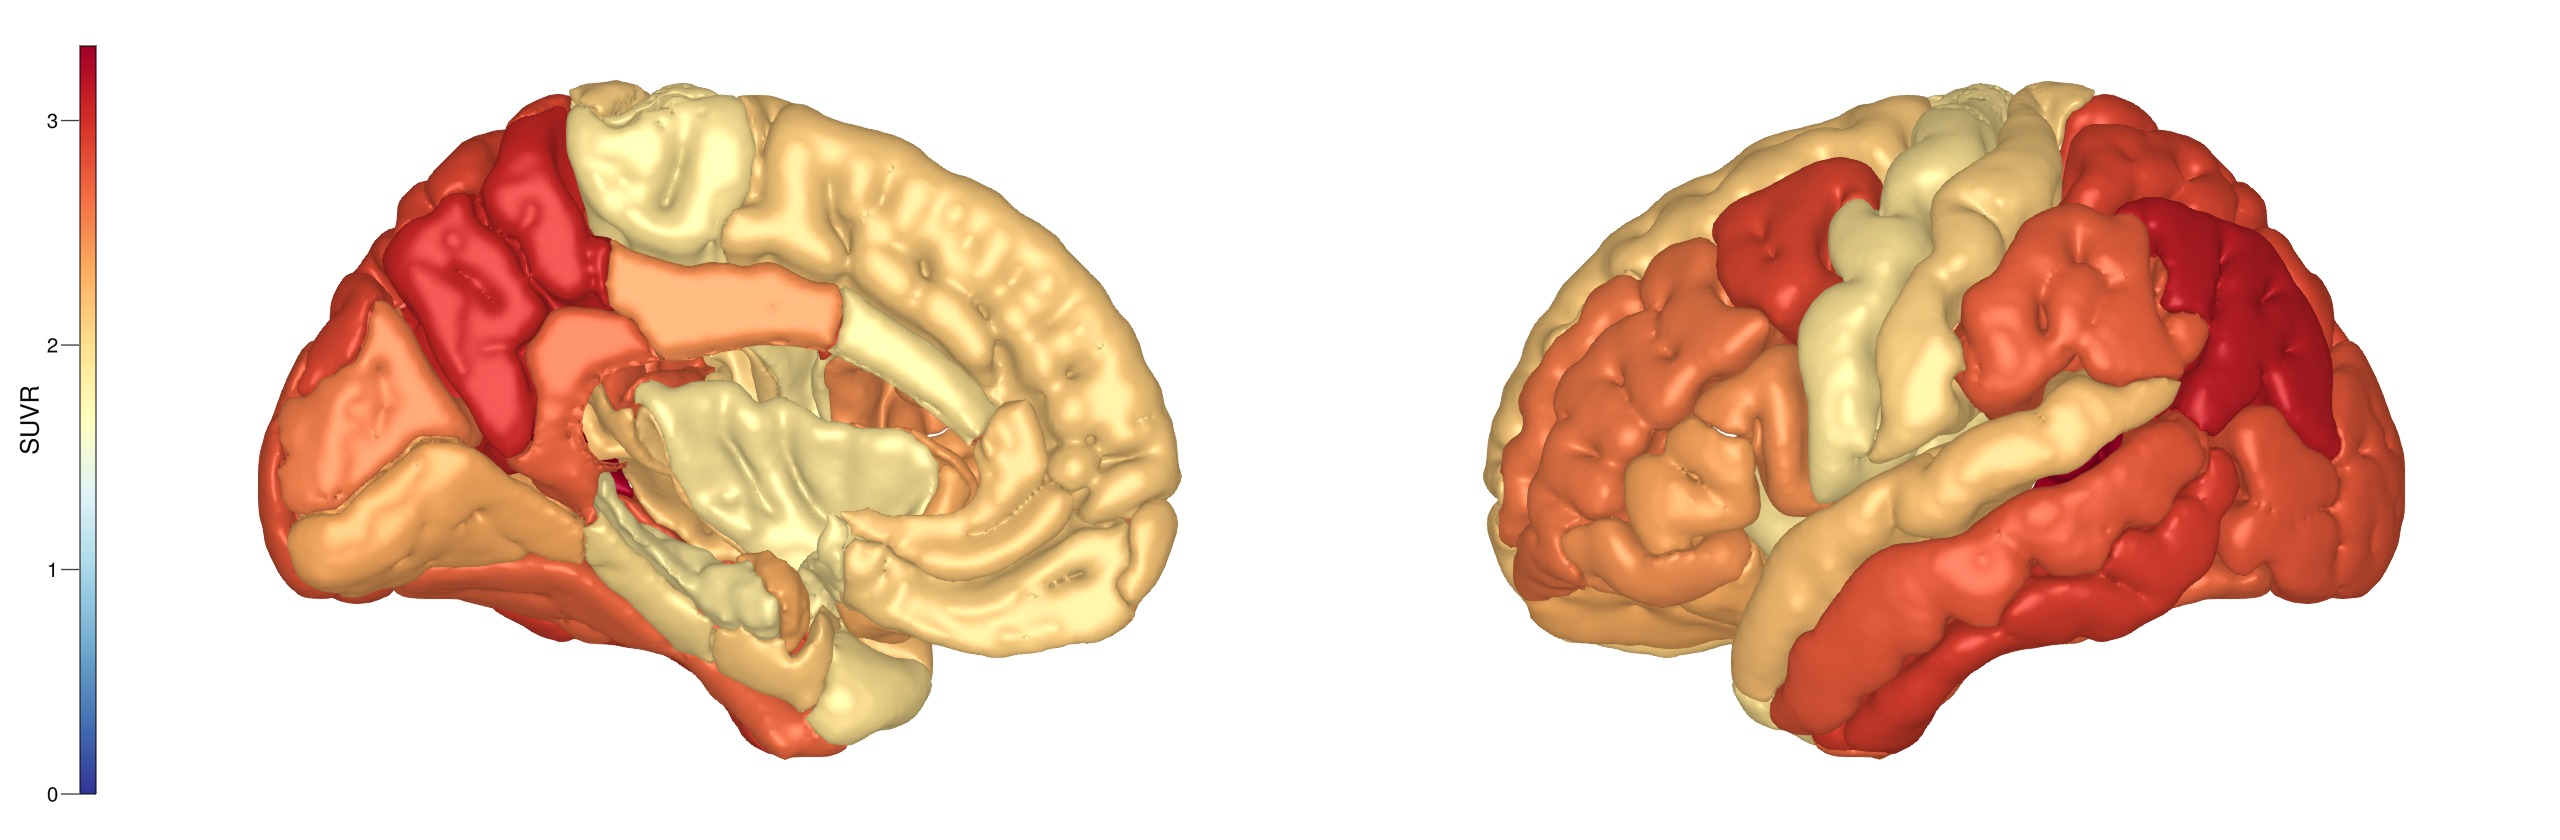
\includegraphics[width=\textwidth]{local-fkpp/models/carrying-capacities.jpeg}
        \caption{Carrying capacity values}
        \label{fig:carrying-capacities}
    \end{subfigure}

    \caption{\textbf{Population level Gaussian mixture modelling}.
    \cref{fig:gmm-lit,fig:gmm-lp} show a two component Gaussian mixture
    model fit to population level SUVR data from the left inferior temporal lobe
    and left putamen, respectively. \cref{fig:baseline-capacities} shows the mean
    of the \TP- negative distribution, $\mathbf{p}_{0}$, on the left hemisphere. 
    \cref{fig:carrying-capacities} shows the 99th percentile of the \TP+ 
    distribution, $\mathbf{p}_\infty$, on the left hemisphere}
    \label{fig:gmm}.
\end{figure}

The simulated dynamics of the local FKPP model, \cref{eqn:fkpp-local}, using the
approximated values of $\mathbf{p}_{0}$ and $\mathbf{p}_\infty$ can be seen in
\cref{fig:fkpp-local}. As with \cref{fig:fkpp-global}, we use synthetic
parameters to illustrate dynamics in a growth dominated regime. The staging
bears close resemblance to Braak staging, namely that with seeding in the
bilateral entorhinal cortex is followed by invasion of the temporal cortices,
followed occipital and frontal regions \cite{cho2016vivo, SCHOLL2016971},
whereas the staging obtained from \cref{eqn:fkpp-global} fails to capture
preferred invasion of frontal regions relative to pre/post central gyrus. The
main difference between the models comes from local variations in growth. In the
time series shown in \cref{fig:fkpp-global}, the concentration at all nodes grow
at the same rate, however, due to the local differences in baseline values and
carrying capacities in the local FKPP model, the concentration at each region
grow at different rates (proportional to the regional carrying capacities),
which can be seen in the time series of \cref{fig:fkpp-local}. As a result, the
model is more representative of observed PET data and the Braak staging we
expect to see in \TP SUVR.

\begin{figure}[H]
    \centering
    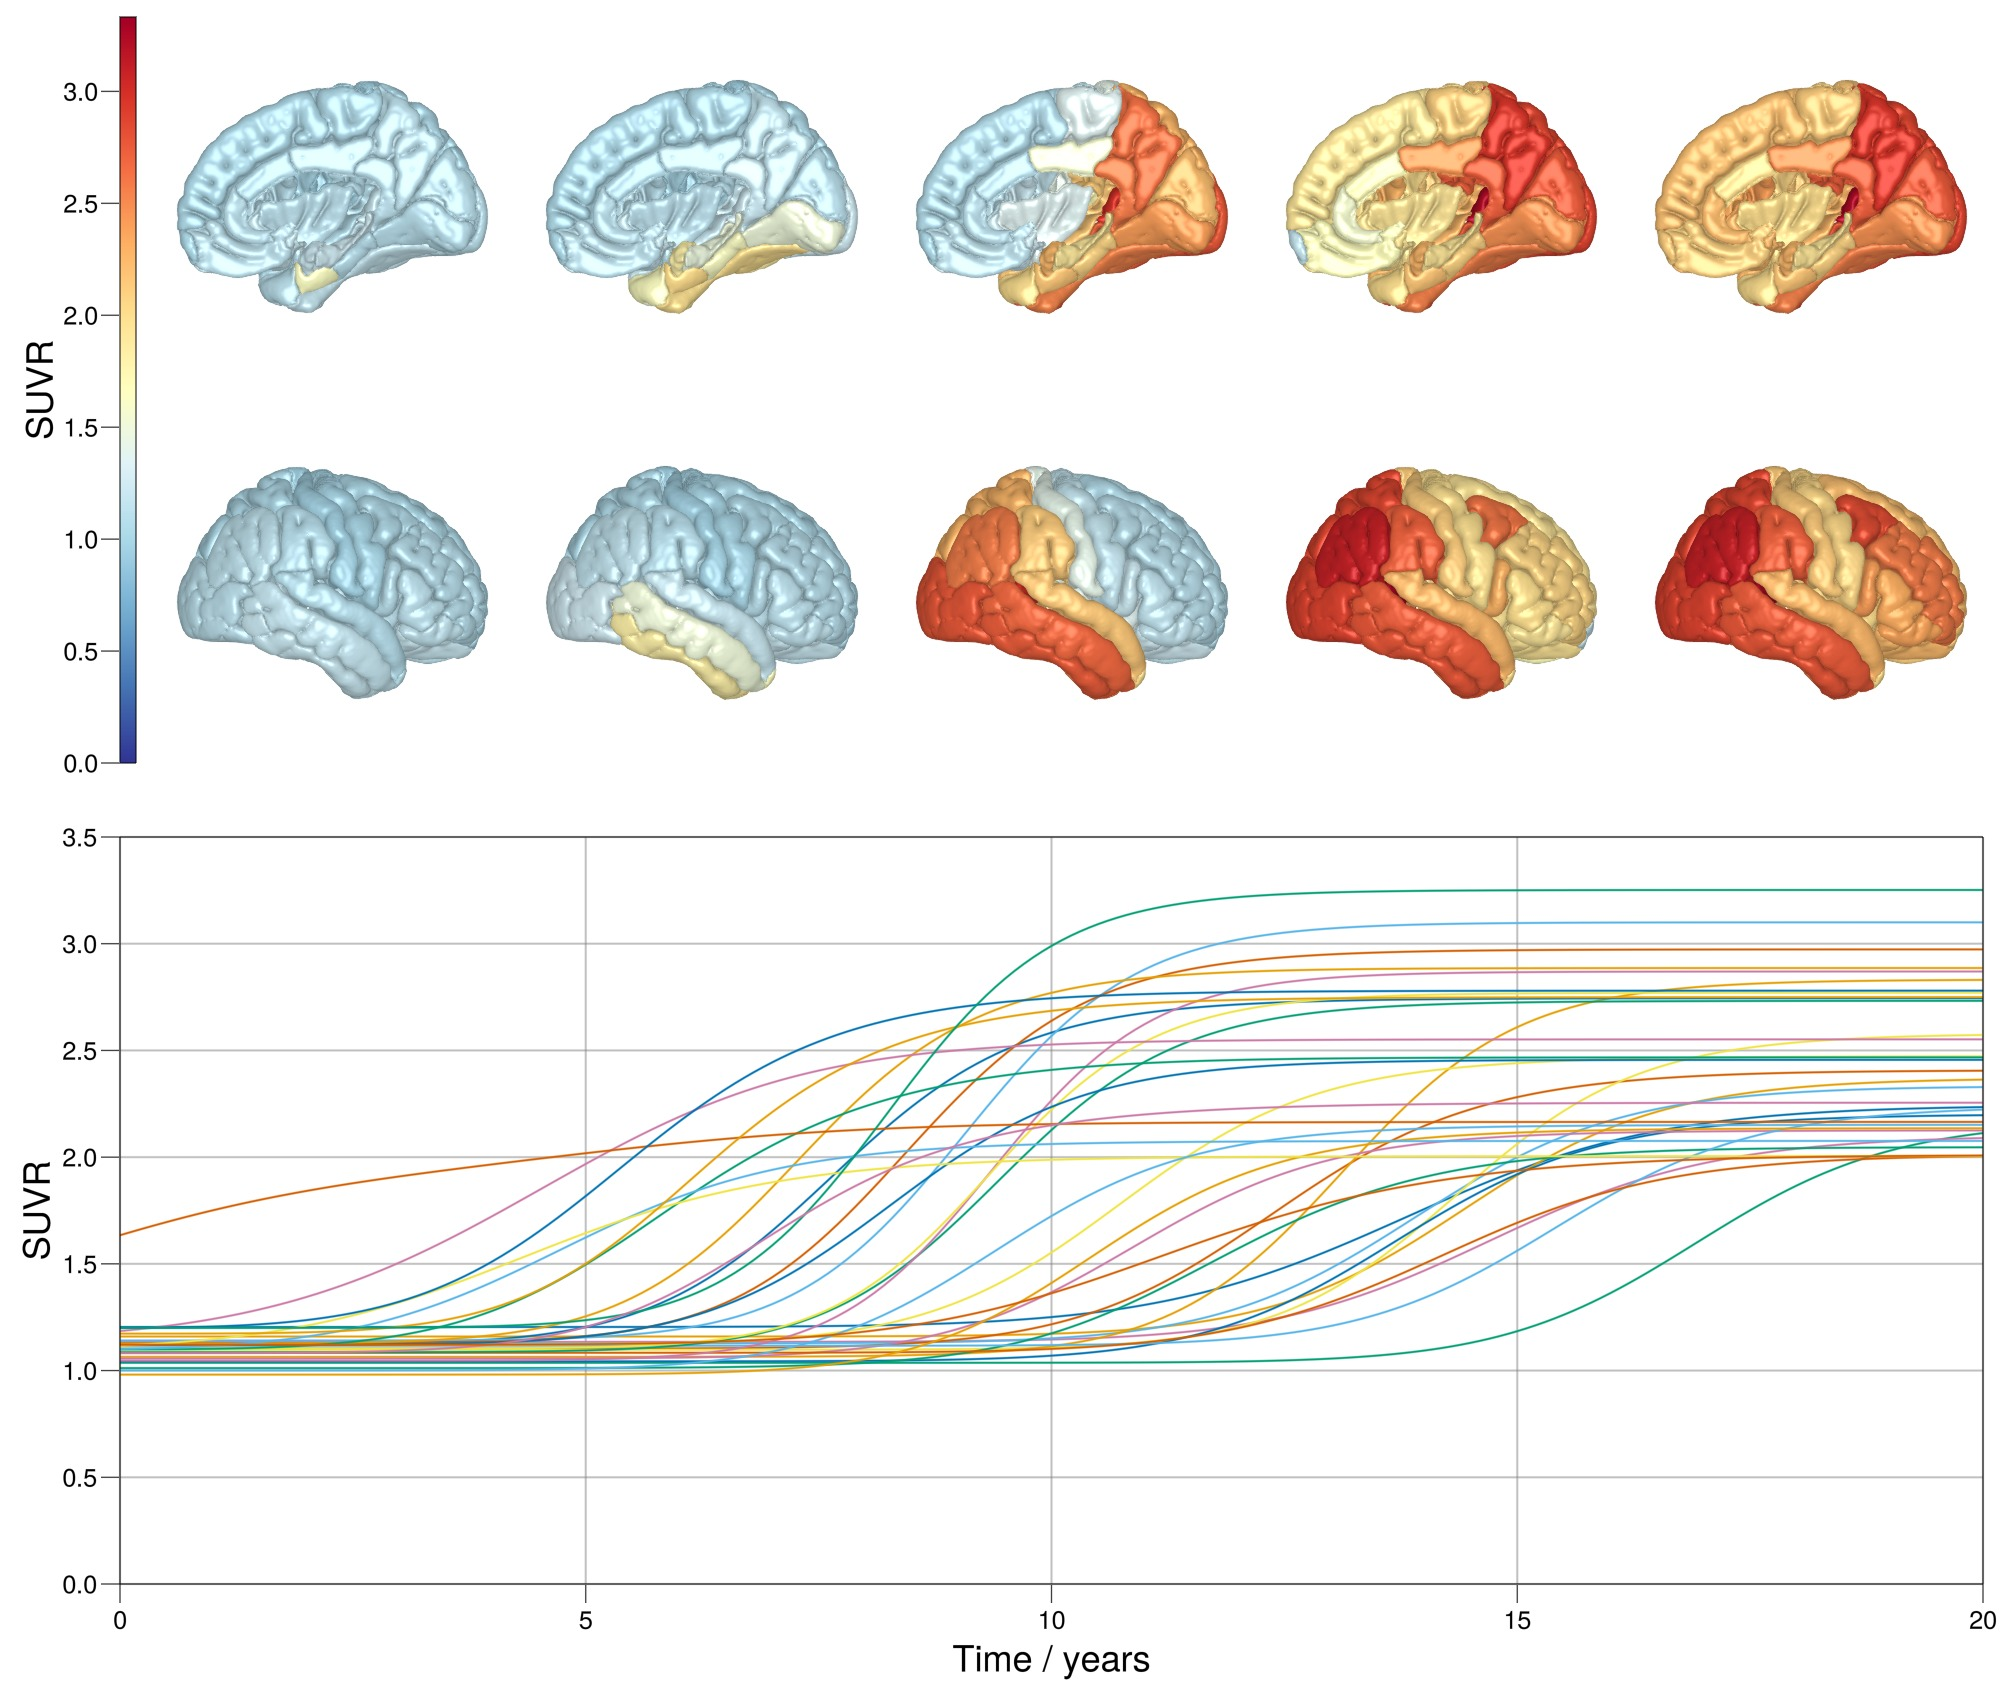
\includegraphics[width=0.9\textwidth]{local-fkpp/models/local-fkpp.jpeg}
    \caption{\textbf{Simulation from the local FKPP model} \cref{eqn:fkpp-local}, 
    with bilateral seeding of 50 percent in the entorhinal cortex, $\rho = 0.2$
    and $\alpha = 1.75$. The seeding concentration is taken as the mean of $p_0$
    and $p_\infty$ for the entorhinal cortex.}
    \label{fig:fkpp-local}
\end{figure}


\section{Identifying Uncertainty}
\label{sec:inference-example}
So far, we have discussed how different models may account for AD. In practice,
one would want to use the models for prediction. In this case, the model
requires calibration to find the most likely parameter values. In a system of
ODEs, the trajectory is uniquely determined by the initial conditions and the
parameters. The process of solving this trajectory is the forward problem. The
inverse problem, which is of concern to us for inference, asks whether the
initial conditions and parameters can be determined from partially observed
trajectories. While traditional frequentist methods have been used in the
literature \cite{raj2015network,vogel2020spread}, here, we will explore Bayesian
inference since it offers a more complete account of uncertainty.

\subsection{Probabilistic Models and Bayesian Inference}

Consider the following data generating process:
\begin{equation}\label{eqn:general-forward-model}
    \tns{x} =  \tns{g}(\tns{u}_0,  \mathbf{t}; \boldsymbol{\theta}, \tns{L}) + \boldsymbol{\epsilon}, 
\end{equation}
where $\tns{x}$ is vector of data that is assumed to be generated by integrating
a function of the form in \cref{equ:general-system}, with initial conditions
$\mathbf{u}_0$ and model parameters, $\boldsymbol{\theta}$, plus measurement
error. Using inference, we hope to identify distributions for unobserved parts
of the system, i.e. model parameters and measurement error. We do this using
Bayesian inference, where the problem corresponds to learning a posterior
density  
$p(\boldsymbol\theta \mid \mathbf{x})$ from a joint probability distribution of
the model and data $p(\boldsymbol\theta , \mathbf{x})$. This is achieved by
making use of the Bayes' theorem.
\begin{equation}\label{eqn:bayesrule}
    \underbrace{p(\boldsymbol{\theta} \mid \mathbf{x})}_{posterior} = 
    \frac{\overbrace{p(\mathbf{x} \mid \boldsymbol{\theta})}^{likelihood}
    \overbrace{p(\boldsymbol{\theta})}^{prior}}
    {\underbrace{p(\mathbf{x})}_{evidence}},
\end{equation}
where $\boldsymbol{\theta}$ is the set of unknown model parameters and $\tns{x}$
are the observations. For even mildly high-dimensional problems, solving for
$p(\boldsymbol\theta, \mid \tns{x})$ becomes intractable using analytic
techniques, since it relies on performing integration over increasingly large
domains to evaluate the evidence term. The evidence term can be reformulated as: 
\begin{equation}
    {p(\mathbf{x})} = \int p(\mathbf{x} , \mathbf{\boldsymbol{\theta}}) \mathrm{d}\mathbf{\boldsymbol{\theta}},
\end{equation}
which shows explicitly that it is necessary to integrate over all of the
dimensions of $\boldsymbol{\theta}$ to compute $p(\tns{x})$. Markov chain Monte
Carlo (MCMC) methods are a popular class of algorithms used for sampling from
the unnormalised posterior distribution, the most common among them being the
Metroplis-Hastings (MH) algorithm. In this work, we use Hamiltonian Monte Carlo
(HMC), an MCMC method that is particularly useful for fast and accurate
inference of high dimensional models with covarying parameters. In general, 
MCMC methods work by sampling from the unnormalised posterior,
denoted $\pi(\boldsymbol\theta)$, which is proportional to the full posterior: 
\begin{equation}
    \label{eqn:unnormalisedpdf}
    \pi(\boldsymbol\theta) = p(\mathbf{x} \mid \boldsymbol{\theta})p(\boldsymbol{\theta}) \propto 
    \frac{p(\mathbf{x} \mid \boldsymbol{\theta})p(\boldsymbol{\theta})}{p(\mathbf{x})}
\end{equation}
To draw samples that capture the posterior, we construct a Markov
process with a transition function $Q(\boldsymbol\theta' \mid
\boldsymbol\theta^t)$, where $\boldsymbol\theta$ is the accepted parameters at
time $t$, and $\boldsymbol\theta'$ are the proposed parameters for $t+1$. Given
certain conditions, this transition function defines a Markov process whose
stationary distribution equals the unnormalised posterior. In random walk MH,
$Q(\boldsymbol\theta' \mid \boldsymbol\theta^t)$ is chosen to be a diagonal
multivariate Normal distribution centred around $\boldsymbol\theta^t$,
$\mathcal{N}(\boldsymbol\theta^t, \boldsymbol\Sigma)$. Proposals
parameters are accepted based on the following if 
\begin{equation}
    u \leq \min\left(1, 
    \frac{\pi(\boldsymbol\theta') Q(\boldsymbol\theta' \mid \boldsymbol\theta^t)}
    {\pi(\boldsymbol\theta) Q(\boldsymbol\theta^t \mid \boldsymbol\theta')}\right)       
\end{equation}
where $u$ is sampled from a uniform distribution, $u \sim \mathcal{U}(0, 1)$,
and rejected otherwise. This Markov process asymptotically converges to the true
posterior distribution as the number of samples tends to infinity. The
transition function used in random walk MH imbues some notable deficiencies that
limit their utility in tackling high dimensional problems. In high dimensional
spaces, the probability that random proposals will be accepted decreases
substantially and therefore the sampler can not efficiently explore posterior
space. This can lead to unfeasibly slow convergence times. HMC obviates this
problem by using a more sophisticated transition function to make proposals. In
HCM the posterior is represented as a Hamiltonian function and proposals are
generated by simulating the dynamics associated with the Hamiltonian. By doing
so the transition function utilises the geometry of posterior space and the
gradients therein to generate samples that have a high probability of being
accepted \cite{betancourt2017conceptual, neal2011mcmc}. This is true even in
high dimensional spaces with highly covarying parameters, making it an attractive
alternative to MH. In the following work we a No-U-Turn-Sampler (NUTS), a HMC
sampler which adaptively finds the optimal step size with which to simulate the
Hamiltonian \cite{hoffman2014no}.

\subsection{An Example Problem}
An example of the probabilistic modelling process is shown in
\cref{fig:fkpp-bayes}. In this example, synthetic data has been generated from
an FKPP model \cref{eqn:fkpp-global}, with an initial protein
concentration seeded in the entorhinal cortex, $\mathbf{u}_0$, shown in
(\cref{fig:fkpp-data}). In this case, the synthetic data has no added noise,
allowing us to test that that the model is identifiable under ideal conditions.
Next, assuming data $\mathbf{x}$ in \cref{eqn:general-forward-model} have
independent and identical Gaussian noise, $\boldsymbol{\epsilon} \sim
\mathcal{N}(0, \sigma^2\mathbf{I})$, our likelihood is given by: 
\[
    p(\mathbf{x} \mid \boldsymbol{\theta}, \sigma, \mathbf{u}_0, \mathbf{t}) = \mathcal{N}(\mathbf{g}(\mathbf{u}_0, \mathbf{t}, \boldsymbol{\theta}, \mathbf{L}), \sigma^2\mathbf{I}).
\]
We can now define priors on the FKPP model parameters, $\theta = \{\rho,
\alpha\}$, and noise parameter, $\sigma$ to define a posterior,
\[
    p(\boldsymbol{\theta}, \sigma \mid \mathbf{x}, \mathbf{u}_0, \mathbf{t}) = p(\mathbf{x} \mid \boldsymbol{\theta}, \sigma, \mathbf{u}_0, \mathbf{t})\,p(\boldsymbol{\theta}, \sigma),
\]
and begin to make use of sampling methods. The prior model encapsulates our
initial beliefs about the data and should generate synthetic data that covers
the observed data. This is seen in \cref{fig:fkpp-prior}, with a truncated
standard normal distribution for $\rho$ and a standard normal prior for
$\alpha$. Trajectories of the FKPP model from the prior are shown in grey and
sufficiently cover the data points, here shown only for the left hippocampus.
With the data and model in place, we use NUTS to sample from the posterior. The
posterior densities can be seen in \cref{fig:fkpp-posterior}. The true values of
the parameters are recovered with very little variation and the posterior
trajectories perfectly capture the observations, indicating that the FKPP model
is identifiable in this idealised case.

\begin{figure}[h]
    \centering
    \begin{subfigure}[b]{0.8\textwidth}
        \centering
        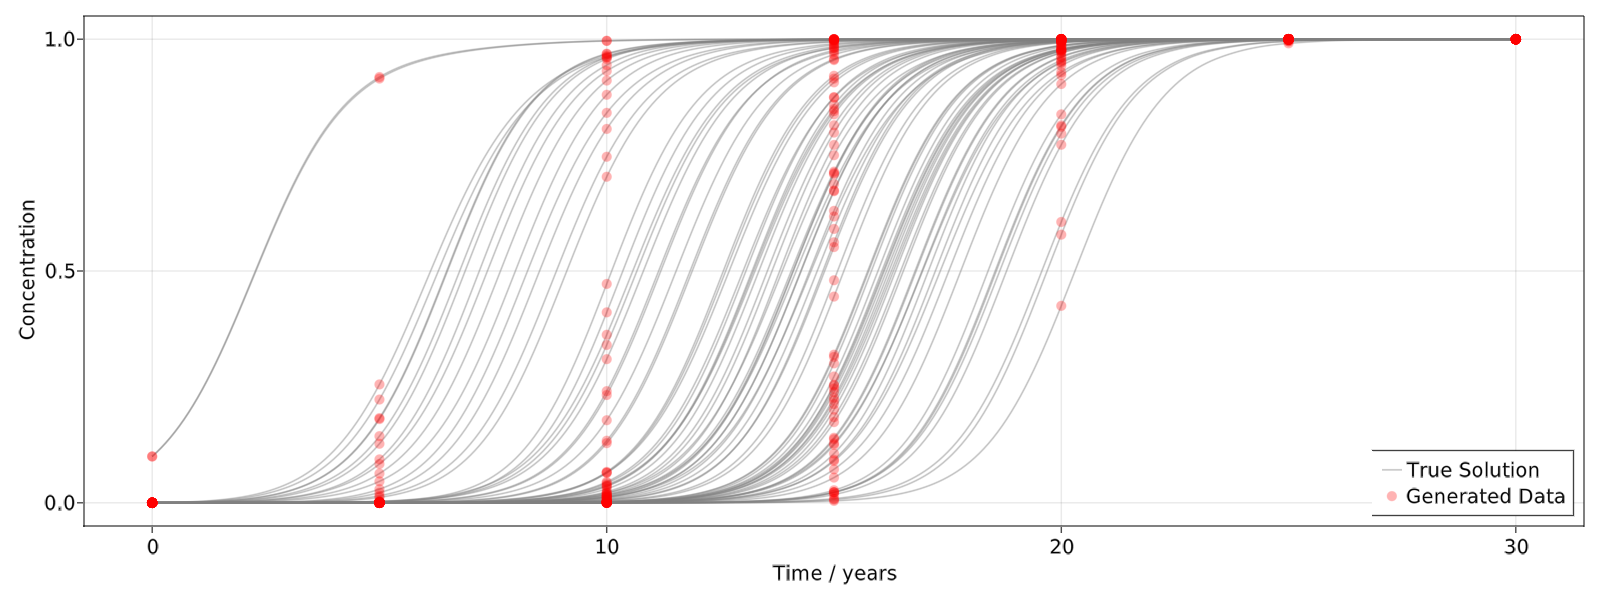
\includegraphics[width=\textwidth]{fkpp/data.png}
        \caption{FKPP solution and synthetic data}
        \label{fig:fkpp-data}
    \end{subfigure}
    \begin{subfigure}[b]{0.8\textwidth}
        \centering
        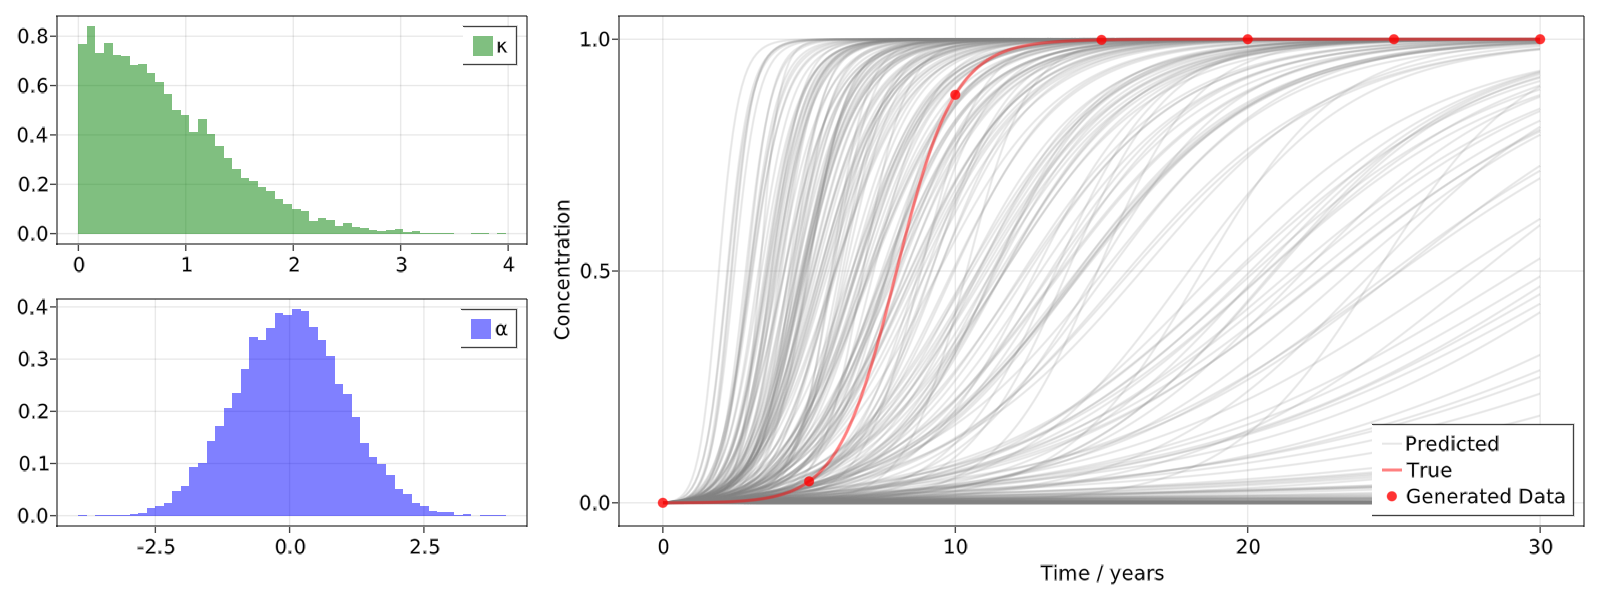
\includegraphics[width=\textwidth]{fkpp/prior_predictive.png}
        \caption{Prior distribution with sample trajectories}
        \label{fig:fkpp-prior}
    \end{subfigure}
    \begin{subfigure}[b]{0.8\textwidth}
        \centering
        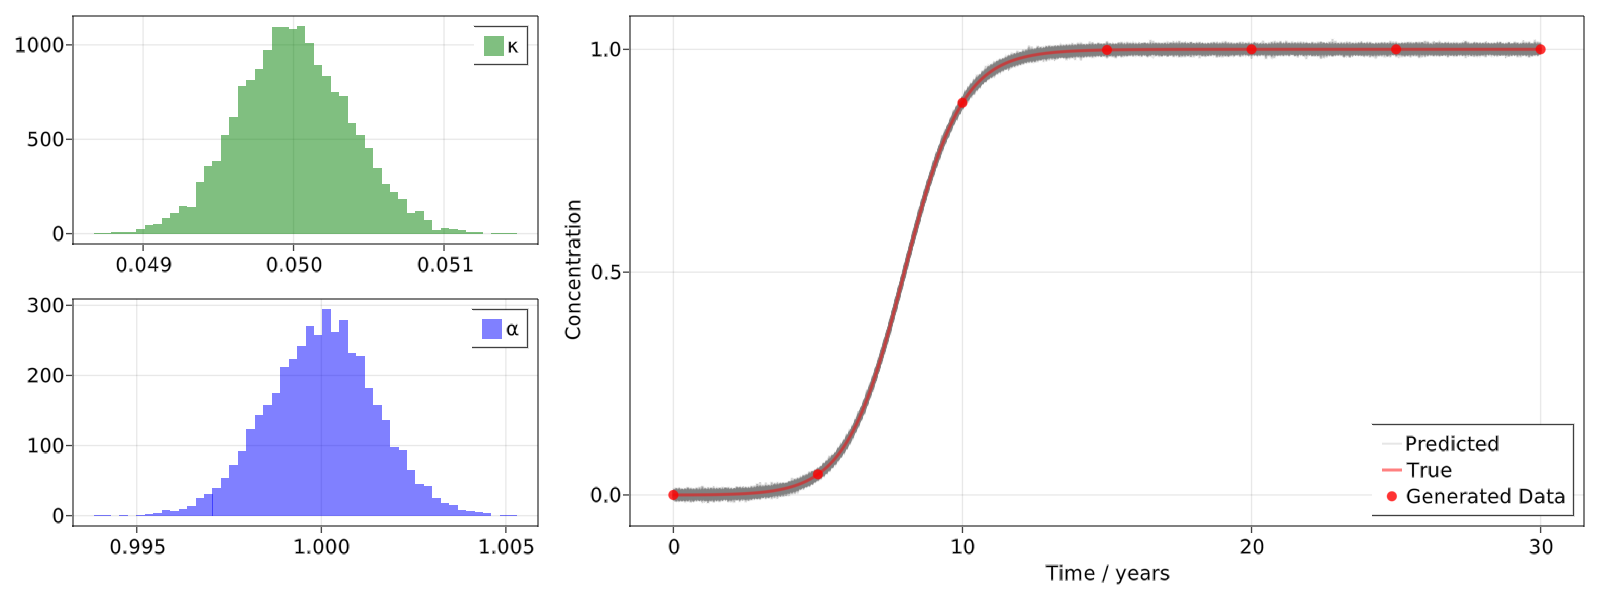
\includegraphics[width=\textwidth]{fkpp/posterior_predictive.png}
        \caption{Posterior distributions with sample trajectories}
        \label{fig:fkpp-posterior}
    \end{subfigure}    

    \caption{\textbf{Probabilistic modelling framework}. \textbf{(a)} Solution to the FKPP model (grey) with initial 
    seeding concentration of 0.1 in the entorhinal cortex, $\rho = 0.05$ and $\alpha = 1.0$, and 
    synthetic data (red) generated by taking solution values at every 5 years. \textbf{(b)} Left: Prior distribution for 
    parameters: $\rho \sim \mathcal{N}^+(0, 1)$, $\alpha \sim \mathcal{N}(0,1)$. Right: FKPP 
    solution trajectories for the right hippocampus using parameters drawn from the prior distributions.
    \textbf{(c)} Left: Posterior distributions obtained using NUTS. Right: FKPP solutions for the right hippocampus 
    using parameters drawn from the posterior distributions.}
        \label{fig:fkpp-bayes}
\end{figure}


\chapter{A Generative Model of Alzheimer's Disease}
\label{chp:3}

\section{Introduction}
\label{sec:introduction}

We have recently shown that shown that a fully Bayesian pipeline can be used to
calibrate spatiotemporal model of AD \cite{schafer2021bayesian,
schafer2022correlating}. The combination of mechanistic mathematical models and
a full Bayesian analysis is attractive for at least two reasons. First,
mechanistic models allow for interpretation and hypothesis-driven investigation.
Secondly, a Bayesian framework provides a natural and robust method for
comparing models and quantifying uncertainty about model structure and
observations. There is yet to be a fully generative approach to
modelling \TP protein dynamics in the brain that accounts for the observation pipeline 
--- this will be the primary contribution of this chapter.

In this chapter, we use \cref{eqn:fkpp-local} presented in \cref{chp:2} and
hierarchical Bayesian inference to compare population level differences between
groups at different stages of AD progression. The calibrated model fits the data
well and our results highlight two interesting differences between patient
groups. First, there is faster transport early in the disease process. Second,
over the course of the disease there is an acceleration in the accumulation rate
of proteins.

\section{Inference using Patient Data}
\label{sec:inference}

Equipped with a dynamical model of \TP SUVR as a function of \TP concentration
\cref{eqn:fkpp-local}, we seek to apply it to patient data and aim to show how
the model describes AD development in patients. We achieve this using data from
two studies, ADNI, which uses the AV1451 radiotracer, and BioFINDER2 (BF2),
which uses RO948 radiotracer \cite{leuzy2020diagnostic}. Since BF2 data are
collected with a different radiotracer, we reapply the methods described in
\cref{sec:regionalparams} to infer fixed regional parameters, $\mathbf{p_0}$ and
$\mathbf{p_\infty}$ specific to this radiotracer. We then apply Bayesian
inference to estimate the posterior distribution over our model parameters given
patient data. We apply inference to different patient groups given by their \AB
and \TP positivity status and show that there is accelerated proteopathy in
patients with a higher \AB and \TP burden.

\subsection{Data Preparation}

Patient data obtained from ADNI are download as fully processed data, summarised
as SUVR values and volumes for each of the regions in the DKT atlas. For details
on the processing methods used, see \cite{landau2016flortaucipir}. We
re-normalise the values using the inferior cerebellum SUVR reference region.
Data from BF2 was provided to us as fully processed data, also with regional
SUVR values and volumes summarised on the DKT atlas. A detailed account of the
processing methods used in BF2 can be found in \cite{OssenkoppeleRik2018DAo1}.
In both ADNI and BF2, we choose only subjects who have at least three \TP PET
scans, allowing us to perform inference on the time-series model. Demographics 
for the selected ADNI and BF2 subjects are given in \cref{table:demo-adni} and 
\cref{table:demo-bf}, respectively.

\begin{table}[h]
    \centering
    \begin{tabular}{lrrrrrr}
      \hline
      \textbf{Group} & \textbf{Age} & \textbf{\% Female} & \textbf{Education} & \textbf{\% CN} & \textbf{\% MCI} & \textbf{\% AD} \\
      \hline
      \ABP \TPP & 75.8 & 0.63 & 16.59 & 0.44 & 0.37 & 0.19 \\
      \ABP \TPN & 79.1 & 0.39 & 16.87 & 0.57 & 0.39 & 0.04 \\
      \ABN & 73.3 & 0.55 & 17.0 & 0.63 & 0.35 & 0.03 \\\hline
    \end{tabular}
    \caption{Cohort demographics for ADNI.}
    \label{table:demo-adni}
\end{table}

\begin{table}[h]
    \centering
    \begin{tabular}{lrrrrrr}
      \hline
      \textbf{Group} & \textbf{Age} & \textbf{\% Female} & \textbf{Education} & \textbf{\% CN} & \textbf{\% MCI} & \textbf{\% AD} \\
      \hline
      \ABP \TPP & 73.9 & 0.65 & 11.6 & 0.2 & 0.43 & 0.37 \\
      \ABP \TPN & 72.1 & 0.5 & 13.2 & 0.61 & 0.31 & 0.08 \\
      \ABN & 66.9 & 0.5 & 12.8 & 0.81 & 0.19 & 0.0 \\\hline
    \end{tabular}
    \caption{Cohort demographics for BF2.}
    \label{table:demo-bf}
\end{table}

For both datasets, we perform inference over three groups, $A\beta^{-}$,
$A\beta^{+} \tau P^{-}$, $A\beta^{+} \tau P^{+}$. In ADNI, \AB status is
determined by an SUVR cutoff value, given in \cite{landau2016florbetapir}. In
BF2, \AB status is again determined by an SUVR cutoff and reported by individual
scanning sites \cite{ossenkoppele2022amyloid}. We distinguish
between $\tau P^{-}$ and $\tau P^{+}$ using a \TP PET SUVR cut-off for two
composite regions, as detailed in \cite{ossenkoppele2022amyloid} and given in
\cref{table:cutoffs}. There are two cut-offs, one for determining \TP
positivity in the medial temporal lobe (MTL), defined as the mean of four
regions, the bilateral entorhinal and amygdala, and another for cortical
positivity, defined as the middle temporal and inferior temporal gyri. The
thresholds for the composite regions are based on regional Gaussian mixture
models. For each composite region, the SUVR  
threshold is defined as mean of the minimum SUVR values at which each subregion
has a greater than $50\%$ probability of belonging to the \TPP distribution. We
define a subject as being \TPP if their last scan is suprathreshold in either
the MTL or cortical \TP PET SUVR and \TPN if the SUVR value is below both SUVR
thresholds. We use two composite regions for cut-off values to account for 
subjects who have atypical AD, presenting with \TP in the cortrex but not the 
medial temporal lobe \cite{vogel2021four}.

\begin{table}[h]
    \centering
    \begin{tabular}{|l|c|c|}
        \hline
        \textbf{Region} & \textbf{ADNI} & \textbf{BF2}  \\
        \hline
        MTL & $1.375$ & $1.248 $\\
        Cortical & $1.395$ & $1.451$  \\
        \hline
    \end{tabular}
    \caption{SUVR threshold values used for defining \TPP and \TPN subjects}
    \label{table:cutoffs}
\end{table}


\subsection{Probabilistic Model}
For each of the three groups, \ABN, \ABP \TPN, \ABP \TPP, we use a hierarchical
model, factoring over patients and scans. In each group there are $N$ subjects,
each of whom have $T_n$ scans, for $n = 1 \hdots N$ subjects, summarised
over 72 regions, $R = 72$. The observations times, i.e. scan dates, are denoted
by $\mathbf{t} = t^{n}_j$ for $j = 1 \hdots T_n$, $n = 1 \hdots N$. We denote
the full data set for a group as $\mathbf{Y}$ and individual subject data as
$Y^{n}_{ij}$, corresponding to the $n^{th}$ subject, at scan $j = 1 \hdots T_n$
and region $i = 1 \hdots R$. For a single subject, we have the following data 
generating function:
\begin{equation}
    \label{eq:generating-function}
    Y^{n}_{ij} = 
    f_i(\mathbf{y_0}^n, \theta^n, t^n_j) + \epsilon_i.
\end{equation}
where $\mathbf{Y}^{n} \in \mathbb{R}^{R \times T_{n}}$, is the data for the
$n^{th}$ subject, $ \mathbf{y}_0 \in \mathbb{R}^{R}$ are their initial
conditions for $R$ regions, $\theta = \{\rho, \alpha\} \in \mathbb{R}^2$ are
subject model parameters, $\mathbf{t} \in \mathbb{R}^{T_{n}}$ are their
observation times. For the initial conditions, $\mathbf{y}_0$, we use the SUVR
values from the subject's first scan. Ideally, we would assume the initial
conditions are also random variables to be inferred, however this would add $N
\times R$ random variables to the model and make sampling infeasible. To derive
a likelihood function from \cref{eq:generating-function}, we assume the
observations errors are independently and identically distributed and sampled
from a Gaussian distribution with standard deviation $\sigma$. The data
generating distribution for a single observation from a subject is then:
\begin{align}
    \epsilon &\sim \mathcal{N}(0, \sigma^2) \\ 
    Y^{n}_{ij} &\sim \mathcal{N}(f_i(\mathbf{y_0}^n, \theta, t^n_j), \sigma^2)
\end{align}
To extend this to a hierarchical population model, we define random variables,
$\Theta = \{(\rho_i, \alpha_i)\}_{i=1}^{N}$, encoding subject specific model
parameters and hierarchical population parameters, $\Omega = \{ \rho_\mu ,
\rho_\sigma, \alpha_\mu, \alpha_\sigma \}$, upon which each $\Theta_i$ depends.
Additionally, there are fixed parameters $\mathbf{y}_0^n \in \mathbb{R}^{R}$ and
$\mathbf{t}^{n} \in \mathbb{R}^{T_{n}}$ for $n = 1 \hdots N$, encoding each
subject's initial conditions and observations times.
\begin{figure}[H]
    \centering
    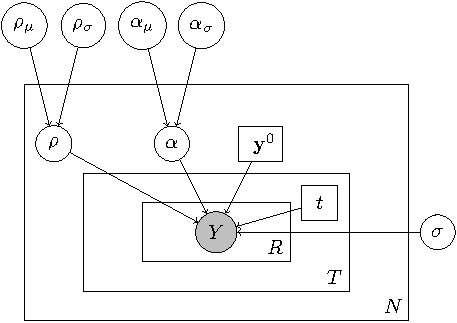
\includegraphics[width=0.75\textwidth]{local-fkpp/inference/plate3.pdf}
    \caption{\textbf{Plate diagram of probabilistic model} showing a graphical
    representation of the hierarchical model used for patient inference.}
    \label{fig:plate}
\end{figure}
A graphical representation of the model is given in \cref{fig:plate}. The
representation of the model as a directed acyclic graph highlights the
conditional dependencies of random variables in the model. From this, we can see
that the likelihood function for a single subject under the hierarchical model
is: 

\begin{equation}
    p(\mathbf{Y}^{n}, \Theta_n \mid \Omega, \sigma, \mathbf{y}_{0}^{n}, \mathbf{t}^{n}) = 
    \prod_j^{T_{n}} \prod_i^R p(Y^{n}_{ij} \mid \Theta_n, \sigma, \mathbf{y}^n_0, t^n_j)
    \,p(\Theta_n \mid \Omega)
\end{equation}
where the first term inside the product on the right hand side is contribution
is the subject level model and the second term is the hierarchical model. The
posterior over hierarchical parameters, subject specific parameters and
observation noise is: 
\begin{equation}
    p(\Theta, \Omega, \sigma \mid \mathbf{Y}, \mathbf{t}, \mathbf{y}_{0})  \propto
    \prod_n^N
    p(\mathbf{Y}^{n}, \Theta_n \mid \Omega, \sigma, \mathbf{y}_{0}^{n}, \mathbf{t}^{n})
    \,p(\Omega, \sigma).
\end{equation}
Next, we perform inference and sample from the posterior distribution to examine 
differences between parameter distributions.


\subsection{Inference over Patient Groups}

\subsection*{Inference Set Up}

We run inference for each patient group separately using a Hamiltonian Monte 
Carlo No-U-Turn Sampler (NUTS). We use the same priors across patient groups; 
these are provided in \cref{table:priors}. We use weakly informative 
priors based on scales at which 
we expect to observe parameter values. The NUTS
sampler is initialised with a unit diagonal Euclidean metric and a target
acceptance ratio of $0.8$. For ADNI data we collected four chains
each with $2000$ samples, and for BF2 data, we collect a single chain of $2000$ 
samples.

\begin{table}[h]
    \centering
    \begin{tabular}{lll}
        \hline
        \textbf{Parameter} & \textbf{Prior} & \textbf{Support} \\
        \hline
        $\rho_\mu$ & $\mathcal{U}(0, 5)$ & $[0, 5]$ \\
        $\rho_\sigma$ & $\Gamma^{-1}(2, 3)$ & $[0, \infty]$ \\
        $\alpha_\mu$ & $\mathcal{U}(-5, 5)$ & $[-5, 5]$ \\
        $\alpha_\sigma$ & $\Gamma^{-1}(2, 3)$ & $[0, \infty]$ \\
        $\rho_i$ & $\mathcal{N}(\rho_\mu, \rho_\sigma)$ & $[0, 5]$ \\
        $\alpha_i$ & $\mathcal{N}(\alpha_\mu, \alpha_\sigma)$ & $[-\infty, \infty]$ \\
        $\sigma$ & $\Gamma^{-}(2,3)$ & $[0, \infty]$\\
        \hline
    \end{tabular}
    \caption{Prior distributions for hierarchical model parameters.}
    \label{table:priors}
\end{table}

\subsection*{Inference Results}

For all patient groups and all chains, we observe good convergence for parameter
distributions in both ADNI and BF2 data. A summary of the hierarchical
parameters is given in \cref{table:pstsummary}. For chain diagnostics, we
report zero divergences in post-warmup samples across all chains, $0.99 \leq
\hat{r} \leq 1.01$, and high effective sample sizes for all parameters.

\subsubsection*{Posterior Distributions}
The hierarchical population parameter distributions are shown in 
\cref{fig:hier-dsts} for ADNI and \cref{fig:hier-dsts-biofinder} for BF2.
There are several interesting observations to be made. First, there is
consistently more uncertainty associated with the \ABN and \ABP \TPN groups,
characterised by the broader distributions for all parameters and higher
parameter values for $\rho_\sigma$ and $\alpha_\sigma$. One contributing factor
to this is the lower signal present in these subjects, increasing the
effect of noise on inference. The higher variance in the \ABP \TPN group may
additionally be explained by higher variance among the subjects, since we only
classify subject inclusion in \TPP or \TPN based on their SUVR relative to the
cut-off values (\cref{table:cutoffs}). It does not take into account
subjects who have have a positive trajectory in \TP SUVR and might have or later
develop tau pathology.

\begin{table}[H]
    \centering
    \begin{tabular}{|r|rr|rr|rr|rr|}
      \hline
      \multirow{2}{*}{\textbf{Group}} &
        \multicolumn{2}{c|}{$\rho_\mu$} &
        \multicolumn{2}{c|}{$\rho_\sigma$} &
        \multicolumn{2}{c|}{$\alpha_\mu$} &
        \multicolumn{2}{c|}{$\alpha_\sigma$} \\
      & mean & s.d. & mean & s.d. & mean & s.d. & mean & s.d.  \\
      \hline
      \ABP \TPP & $0.0357$ & $0.0317 $ & $0.2965$ & $0.0544$ & $0.1277$ & $0.0359$ & $0.1856$ & $0.0309$  \\

      \ABP \TPN & $0.1871$ & $0.1514$ & $0.8076$ & $0.1787$ & $-0.0520$ & $0.1003$ & $0.4248$ & $ 0.0796$ \\

      \ABN & $0.0616$ & $0.0543$ & $0.4780$ & $0.0838$ & $-0.1346$ & $0.0504$ & $0.2937$  & $ 0.0446 $ \\
      \hline
    \end{tabular}
    \caption{\textbf{Posterior Summary: ADNI} Means of hierarchical population parameters.}
    \label{table:pstsummary}
\end{table}

\begin{table}[H]
    \centering
    \begin{tabular}{|r|rr|rr|rr|rr|}
      \hline
      \multirow{2}{*}{\textbf{Group}} &
        \multicolumn{2}{c|}{$\rho_\mu$} &
        \multicolumn{2}{c|}{$\rho_\sigma$} &
        \multicolumn{2}{c|}{$\alpha_\mu$} &
        \multicolumn{2}{c|}{$\alpha_\sigma$} \\
      & mean & s.d. & mean & s.d. & mean & s.d. & mean & s.d.  \\
      \hline
      \ABP \TPP & $0.0114$ & $0.0107$ & $0.1693$ & $ 0.0235$ & $0.1104 $ & $0.0167$ & $0.1202$ & $0.0143$  \\

      \ABP \TPN & $0.2726$ & $0.2430$ & $1.5019$ & $0.4574$ & $0.0142$ & $0.0613$ & $0.2687$ & $0.0513$ \\

      \ABN & $0.0700$ & $0.0697$ & $1.1070$ & $0.1475$ & $-0.0569$ & $0.0314$ & $0.2131$  & $0.0259$ \\
      \hline
    \end{tabular}
    \caption{\textbf{Posterior Summary: BF2}    Means of hierarchical population parameters.}
    \label{table:pstsummary-bf}
\end{table}

The posterior distributions also inform us on the global dynamical regimes
across different stages of AD progression, where a diffusion dominated regime is
given when $ \rho \ll \alpha $, form and a growth dominated regime when $ \rho
\gg \alpha$ (in dimensionless form). The dimensionless parameters are given in
\cref{table:pstsummary} for ADNI \cref{table:pstsummary-bf} for BF2.
In both datasets the inferred parameters suggest that the transport of toxic
proteins in \ABN and \ABP \TPP are decay/growth dominated, $ \rho_\mu \ll
\alpha_\mu $, but in \ABP \TPP it is diffusion dominated $ \rho_\mu \gg
\alpha_\mu $. This suggests that during early disease, proteins are transported
around the brain network more than in later stage AD, where pathology is
primarily driven by growth, as evidenced by the higher growth parameter in the
\ABP \TPP group.

Lastly, the growth parameter increases depending on the AD group, from \ABN to
\ABP \TPN and finally to \ABP \TPP. This result has two implications. First, AD
pathology depends on the presence of toxic \AB, evident by the positive growth
rates estimated in the \ABP groups and predominantly negative growth in the \ABN
group. Secondly, as AD progresses, there is an acceleration of toxic \TP
accumulation, seen by the increased growth rates of toxic \TP in the \ABP \TPP
group compared to the \ABP \TPN group.

\begin{figure}[H]
    \centering
    \begin{subfigure}{0.8\textwidth}
        \centering
        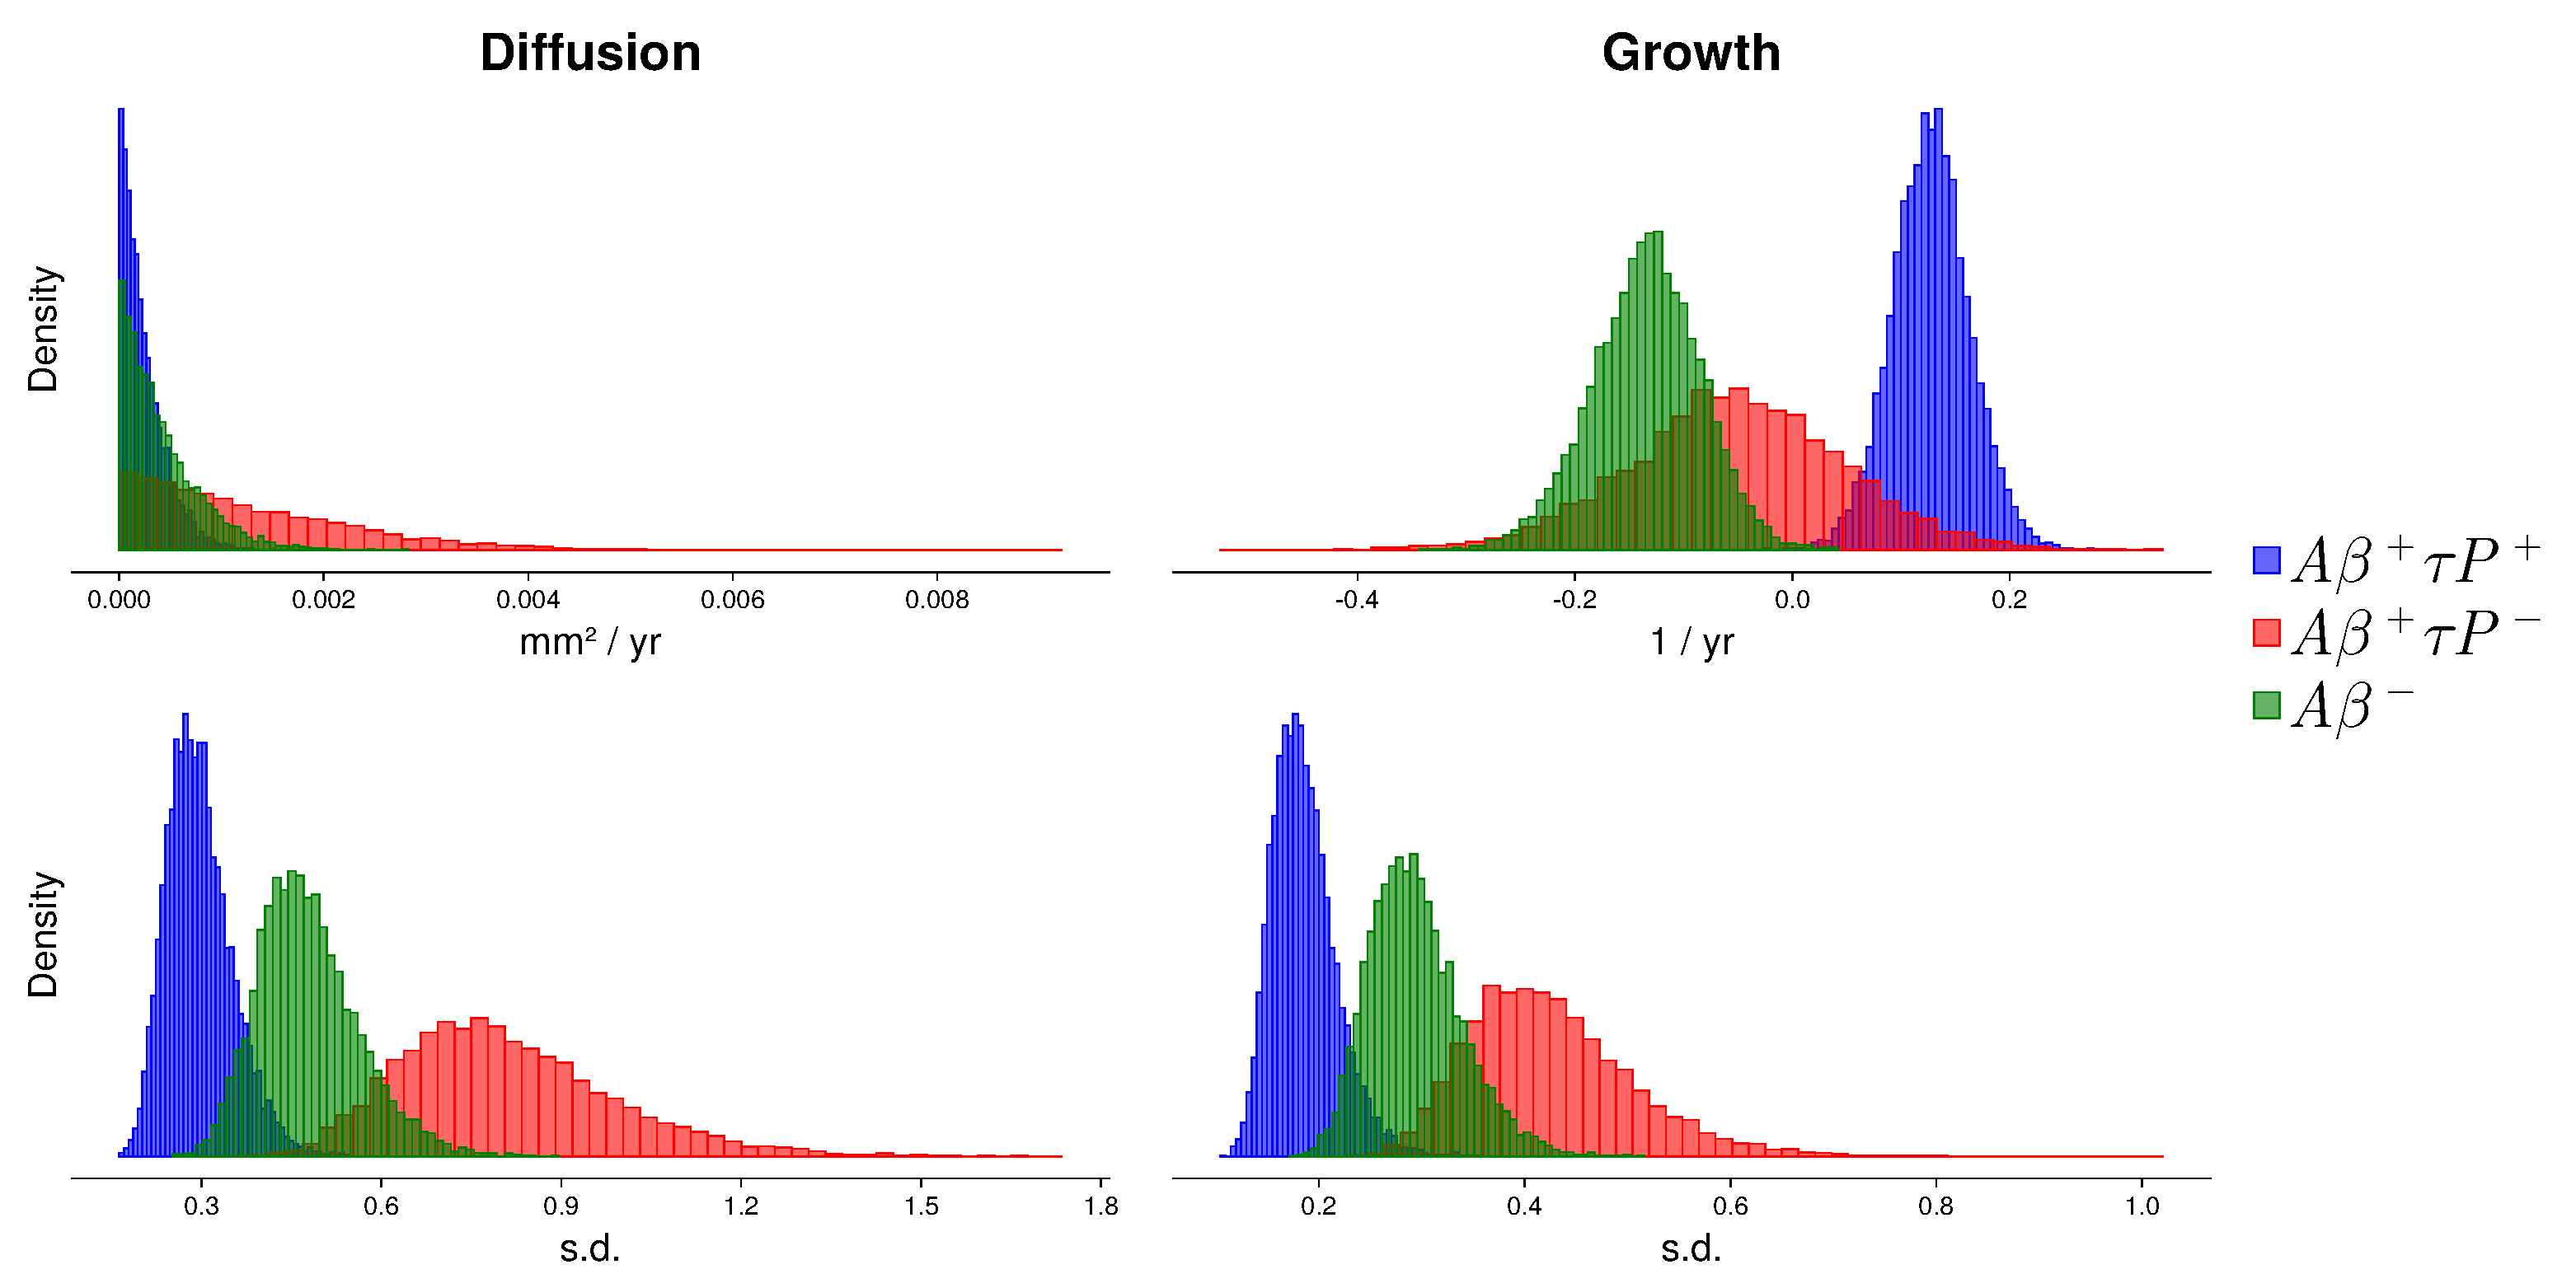
\includegraphics[width=\textwidth]{local-fkpp/inference/hier-dsts.pdf}
        \caption{Distributions of hierarchical population model parameters.}
        \label{fig:hier-dsts}
    \end{subfigure}

    \begin{subfigure}{0.8\textwidth}
        \centering
        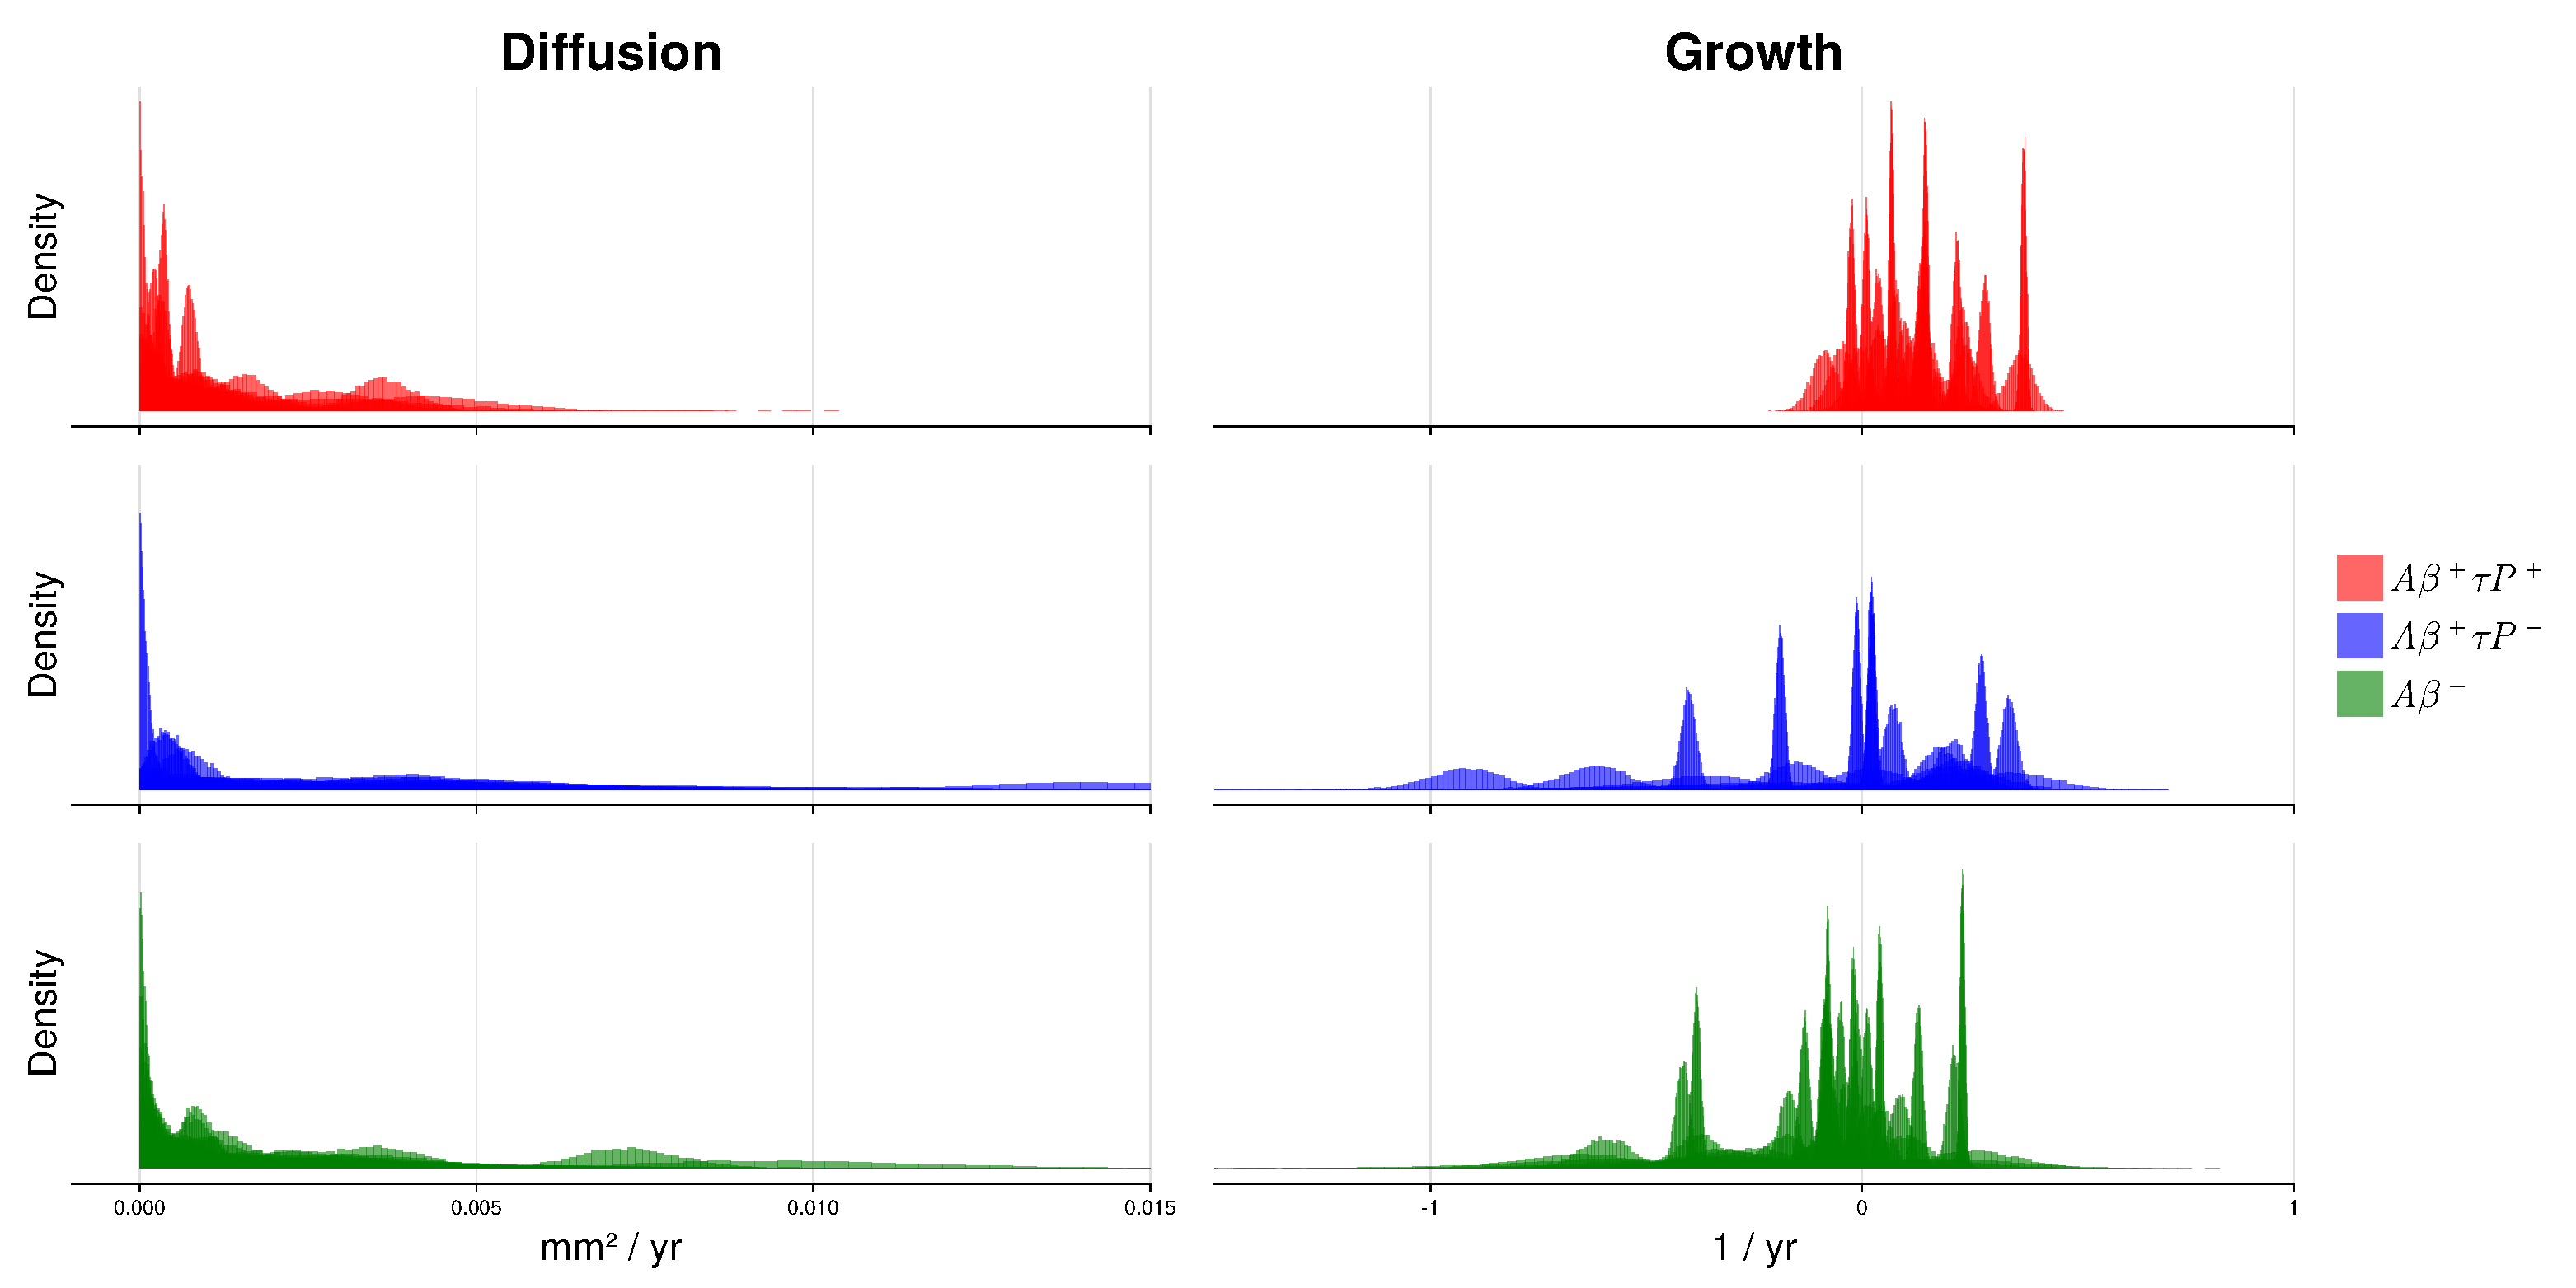
\includegraphics[width=\textwidth]{local-fkpp/inference/sub-dsts.pdf}
        \caption{Distributions of individual model parameters.}
        \label{fig:sub-dsts}
    \end{subfigure}
    
    \caption{\textbf{Posterior distributions from ADNI data.} 
    Inferred posterior distributions for hierarchical population model
    parameters and individual model parameters.}
    \label{fig:inferred-dsts}
\end{figure}

\begin{figure}[H]
    \centering
    \begin{subfigure}{\textwidth}
        \centering
        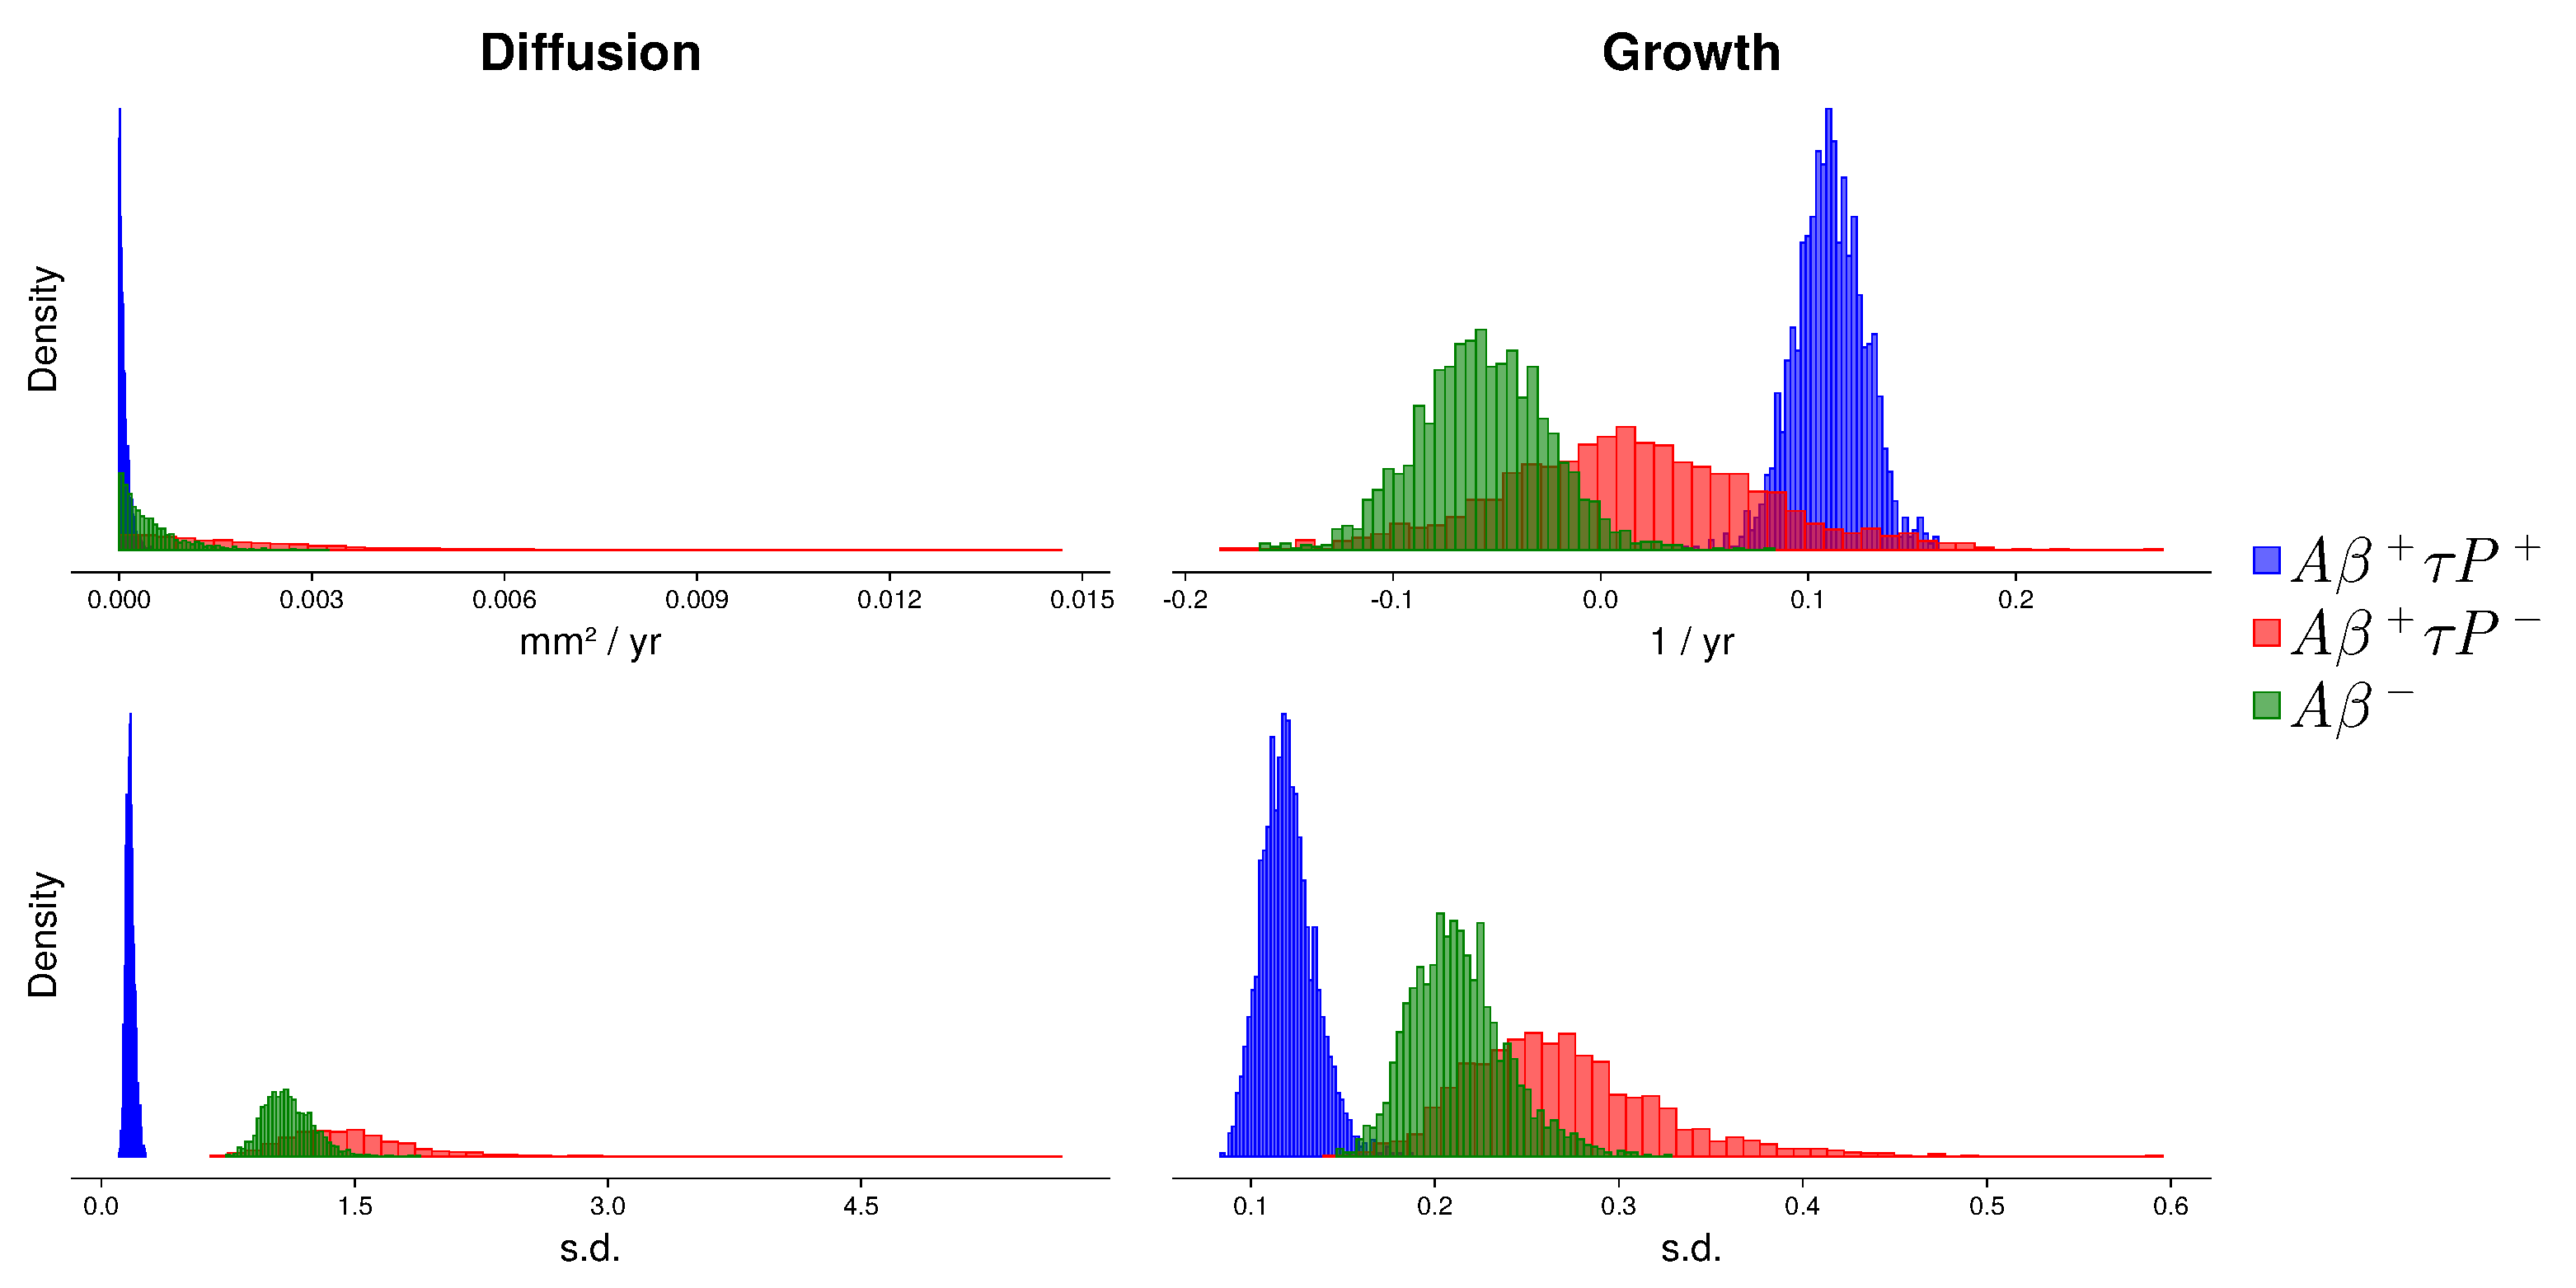
\includegraphics[width=\textwidth]{biofinder/hier-dsts-2000-fd-065-c99.pdf}
        \caption{Distributions of hierarchical population model parameters.}
        \label{fig:hier-dsts-biofinder}
    \end{subfigure}

    \begin{subfigure}{\textwidth}
        \centering
        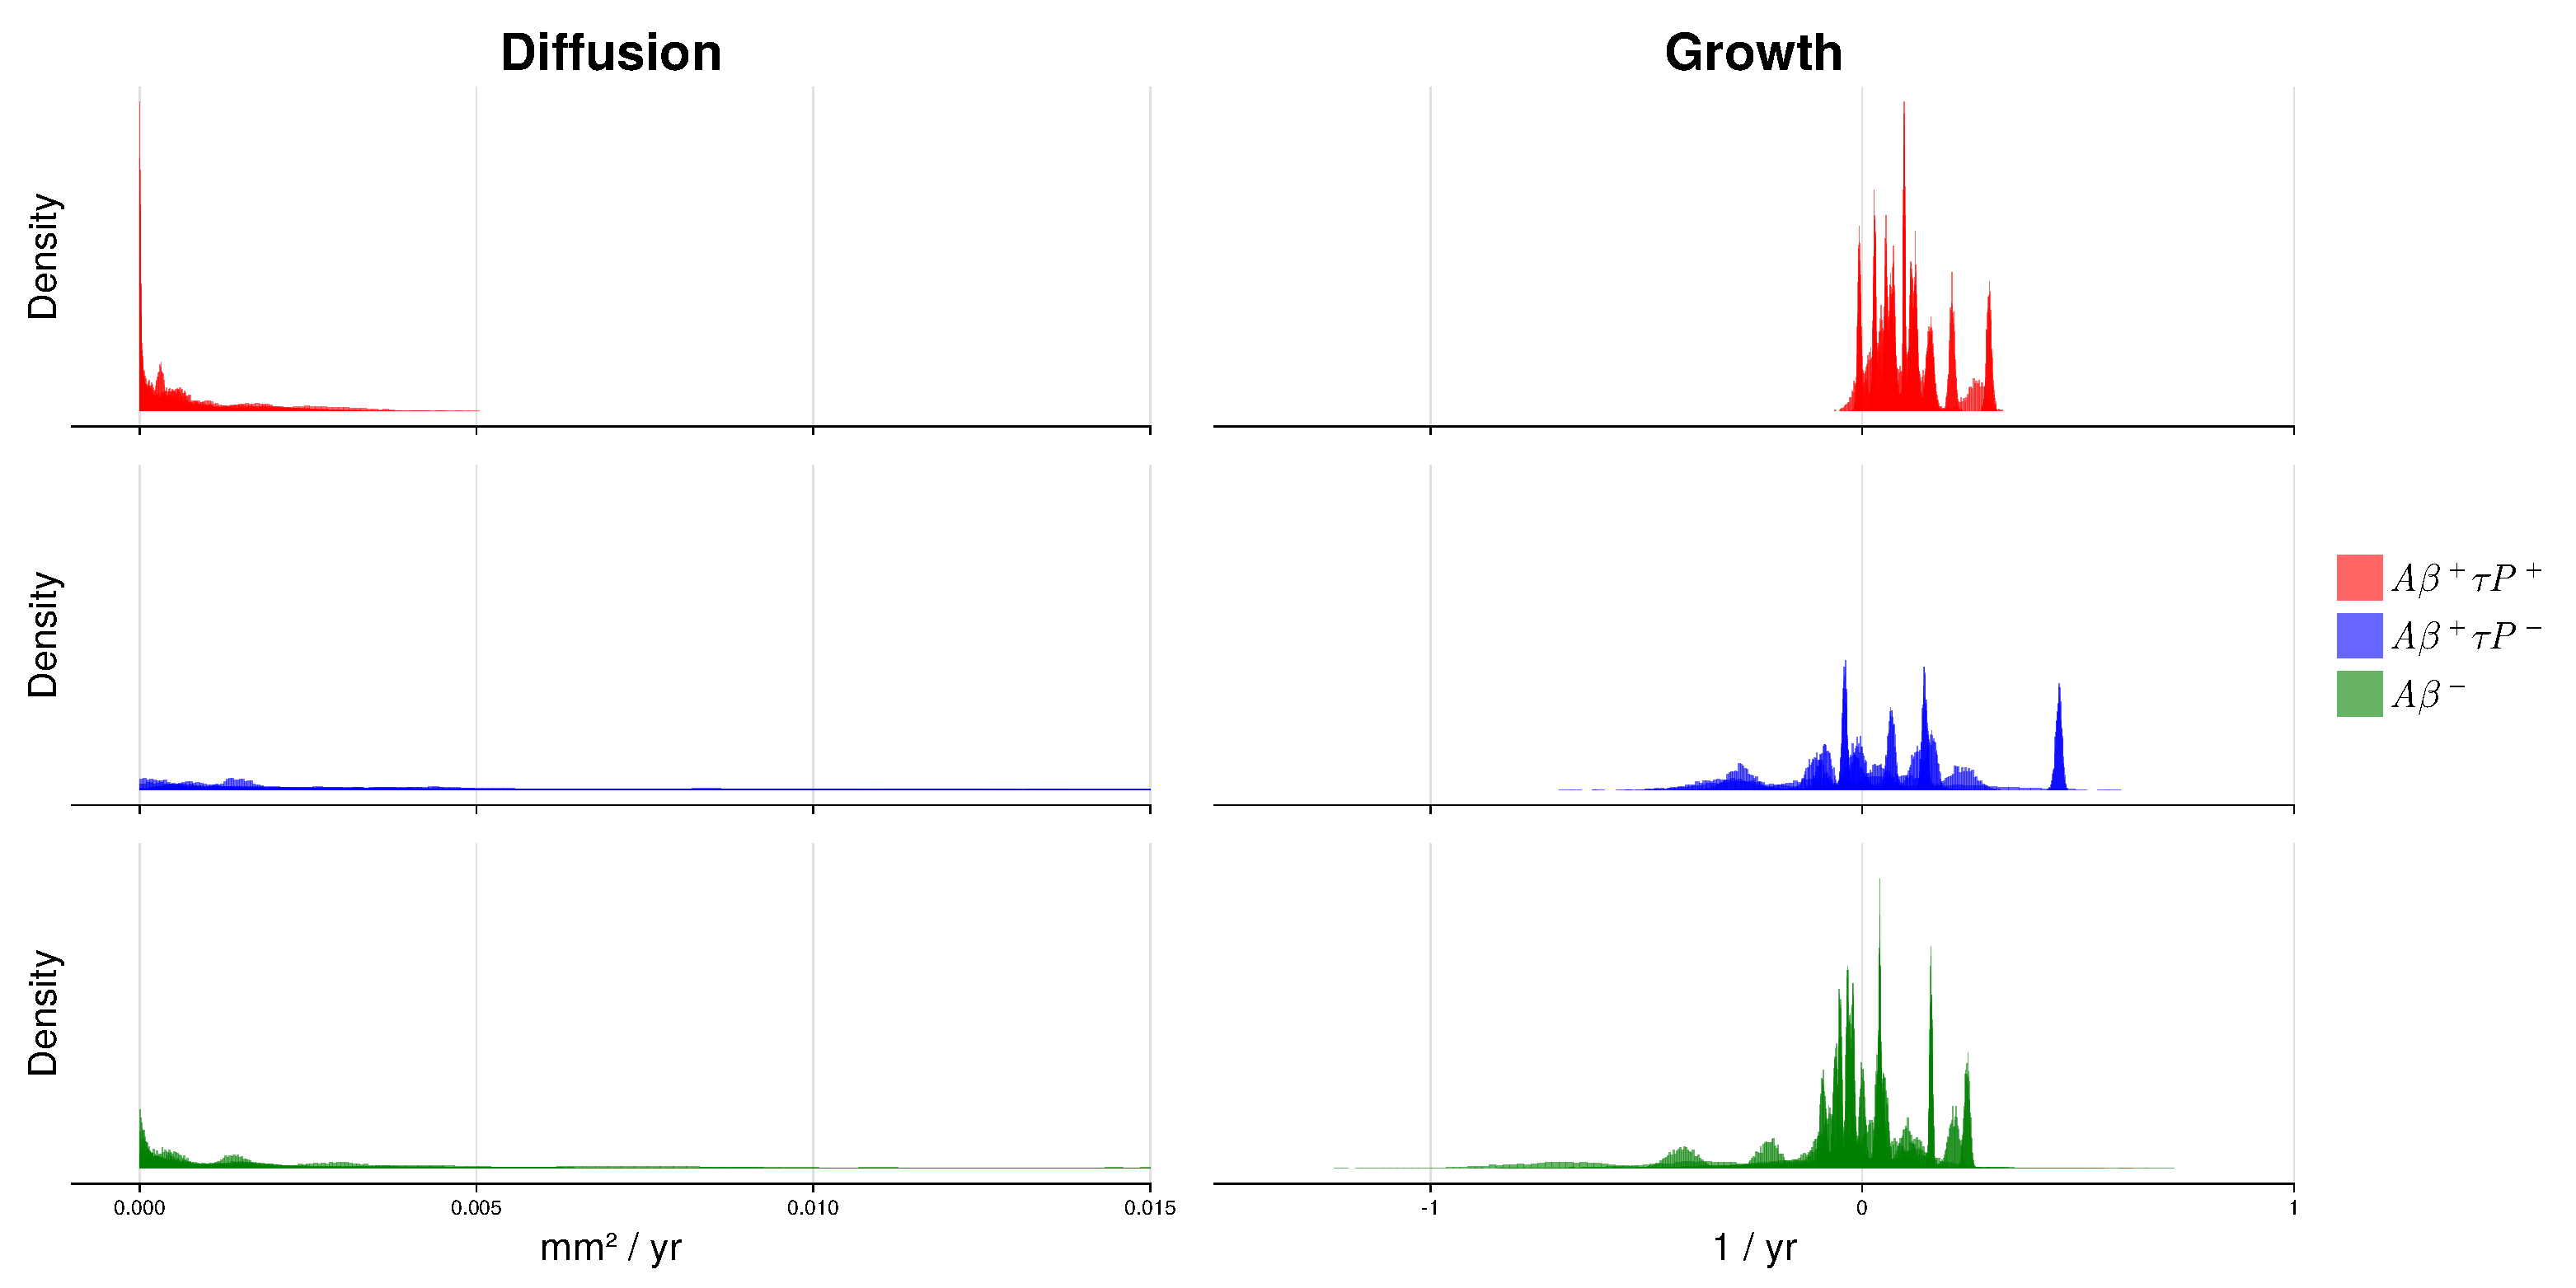
\includegraphics[width=\textwidth]{biofinder/sub-dsts-2000-fd-065-c99.pdf}
        \caption{Distributions of individual model parameters.}
        \label{fig:sub-dsts-biofinder}
    \end{subfigure}
    
    \caption{\textbf{Posterior distributions from BF2.} 
    Inferred posterior distributions for hierarchical population model
    parameters and individual model parameters.}
    \label{fig:inferred-dsts-biofinder}
\end{figure}

\subsubsection*{Posterior Predictive Simulations}

Using the posterior distributions, we can generate samples from the posterior
predictive distributions to assess the goodness of fit and uncertainty in
predictions. Simulations from the \TPP group are shown in
\cref{fig:pstpred-taupos-it,fig:pstpred-taupos-ec} for ADNI, showing data and
simulations from the right inferior temporal lobe and right entorhinal cortex,
respectively, and \cref{fig:pstpred-taupos-it-bf,fig:pstpred-taupos-ec-bf} for
BF2. Similarly, simulations from the \TPN group are shown in
\cref{fig:pstpred-tauneg-it,fig:pstpred-tauneg-ec} for ADNI, and
\cref{fig:pstpred-tauneg-it-bf,fig:pstpred-tauneg-ec-bf} for BF2. Generally, the
calibrated models fit the data very well, and it can be seen that the \TPP
subjects typically have disease progression, whereas \TPN subjects are more
likely to decline, remain stable, or increase more slowly and with greater
uncertainty. 

There are some data points that are not captured within the confidence
intervals. There are a few reasons why data points might not be captured by the
calibrated model. First, we have used a hierarchical model to group information
across subjects and to limit over-fitting through shrinkage, this includes
grouping together observation noise into a single noise parameter. Secondly,
although we have used some regional information in the form of local \p0 and \pI
values, we still have a global growth parameter, $\alpha$, which may prevent
regional trajectories from capturing data points so as to maximise the fit
across all regions. Thridly, we have not incorporated uncertainty around the
initial conditions, which are taken as the SUVR values at the first observation.
This introduces potentially large variations into the forward simulations and
could account for some data points not being captured. Finally, our model is
incapable of describing non-monotonic trajectories and therefore cannot capture
variations in data that might be explained by short-time fluctuations in \TP
concentration, due to clearance or volume atrophy. An example of this can be
seen in the bottom left image of \cref{fig:pstpred-taupos-ec}, where there is a
marked decline in SUVR but increase in the right inferior temporal lobe of same
subject in \cref{fig:pstpred-taupos-it}. Given that the SUVR value in the
entorhinal cortex is close to the carrying capacity, this is likely due to
atrophy of the entorhinal cortex, known to be among the first regions to
degenerate, and therefore a decreasing SUVR. Future work should aim to address 
these limitations, particularly those stemming from simplifying assumptions, to 
provide a more complete method for predicting single subject trajectories.

\begin{figure}[H]
    \centering
    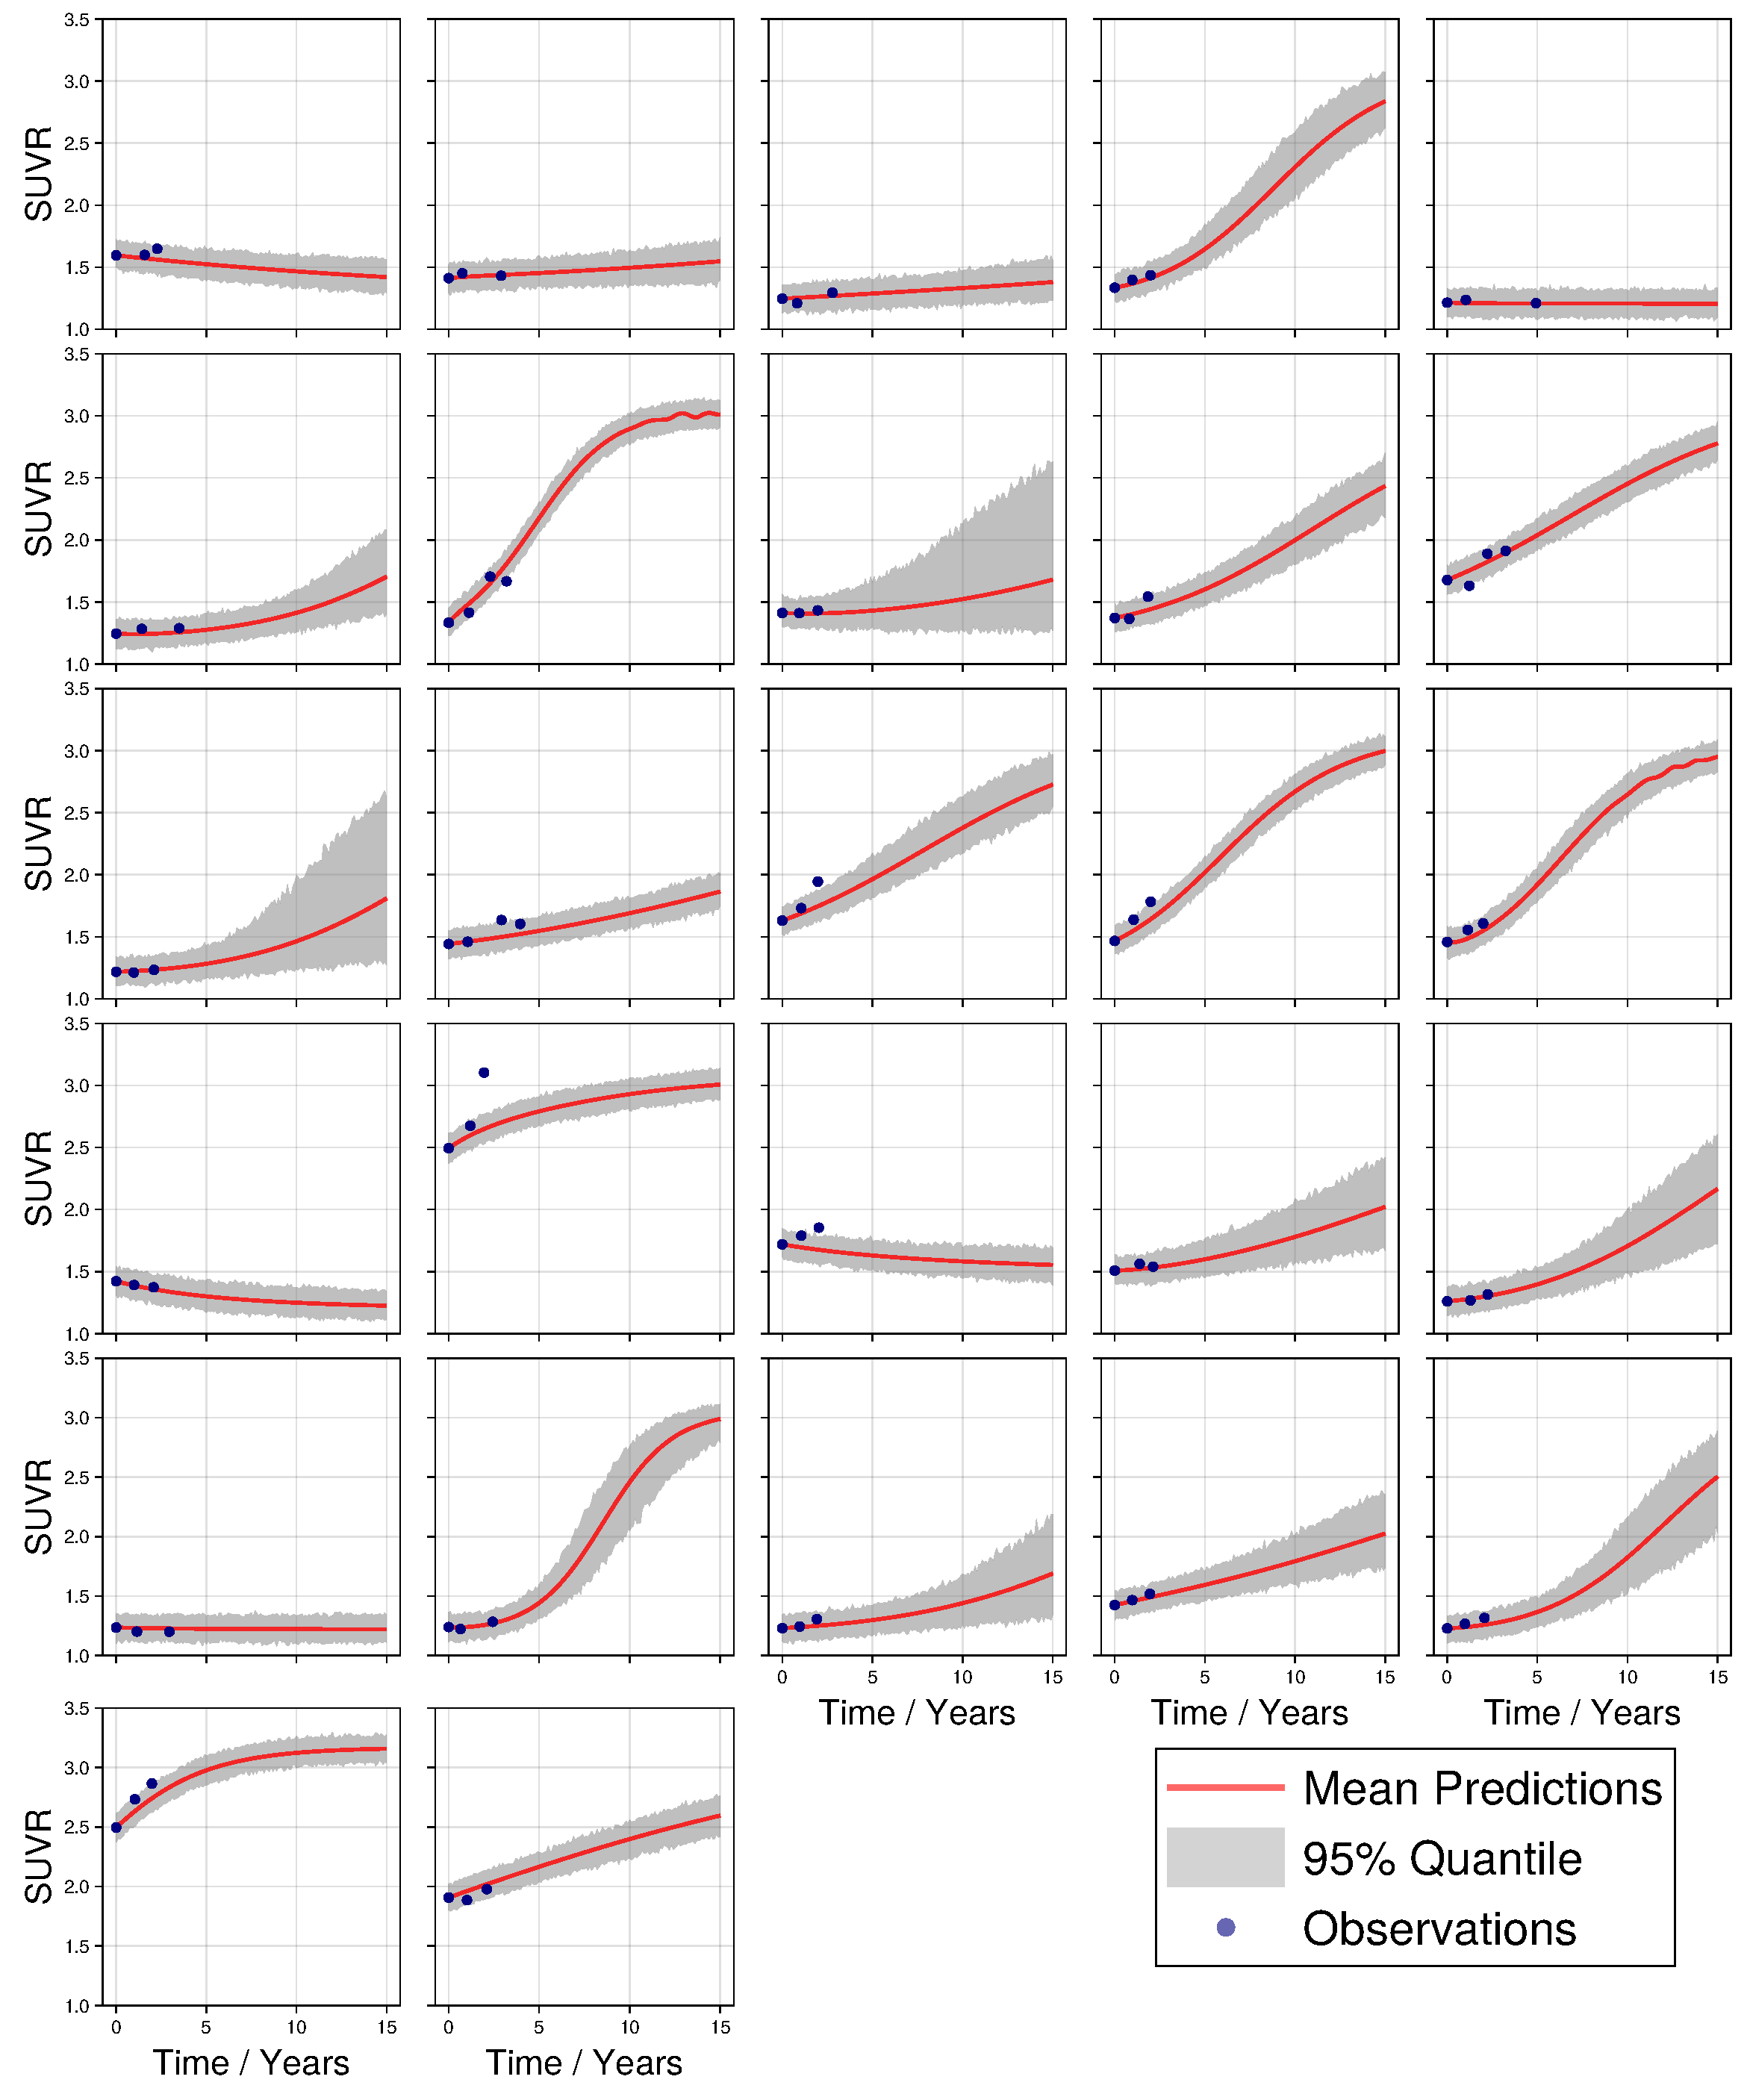
\includegraphics[width=1.0\textwidth]{local-fkpp/inference/pstpred-taupos-inferiortemporal.pdf}
    \caption{\textbf{Posterior predictive trajectories for the right inferior
    temporal lobe in ADNI \ABP \TPP}Forward simulations from the posterior
    distributions of the \TPP group. Shown here are data (blue scatter points)
    and simulated trajectories (mean predictions in red and 95\% confidence
    intervals in grey) from the right inferior temporal lobe.}
    \label{fig:pstpred-taupos-it}
\end{figure}

\begin{figure}[H]
    \centering
    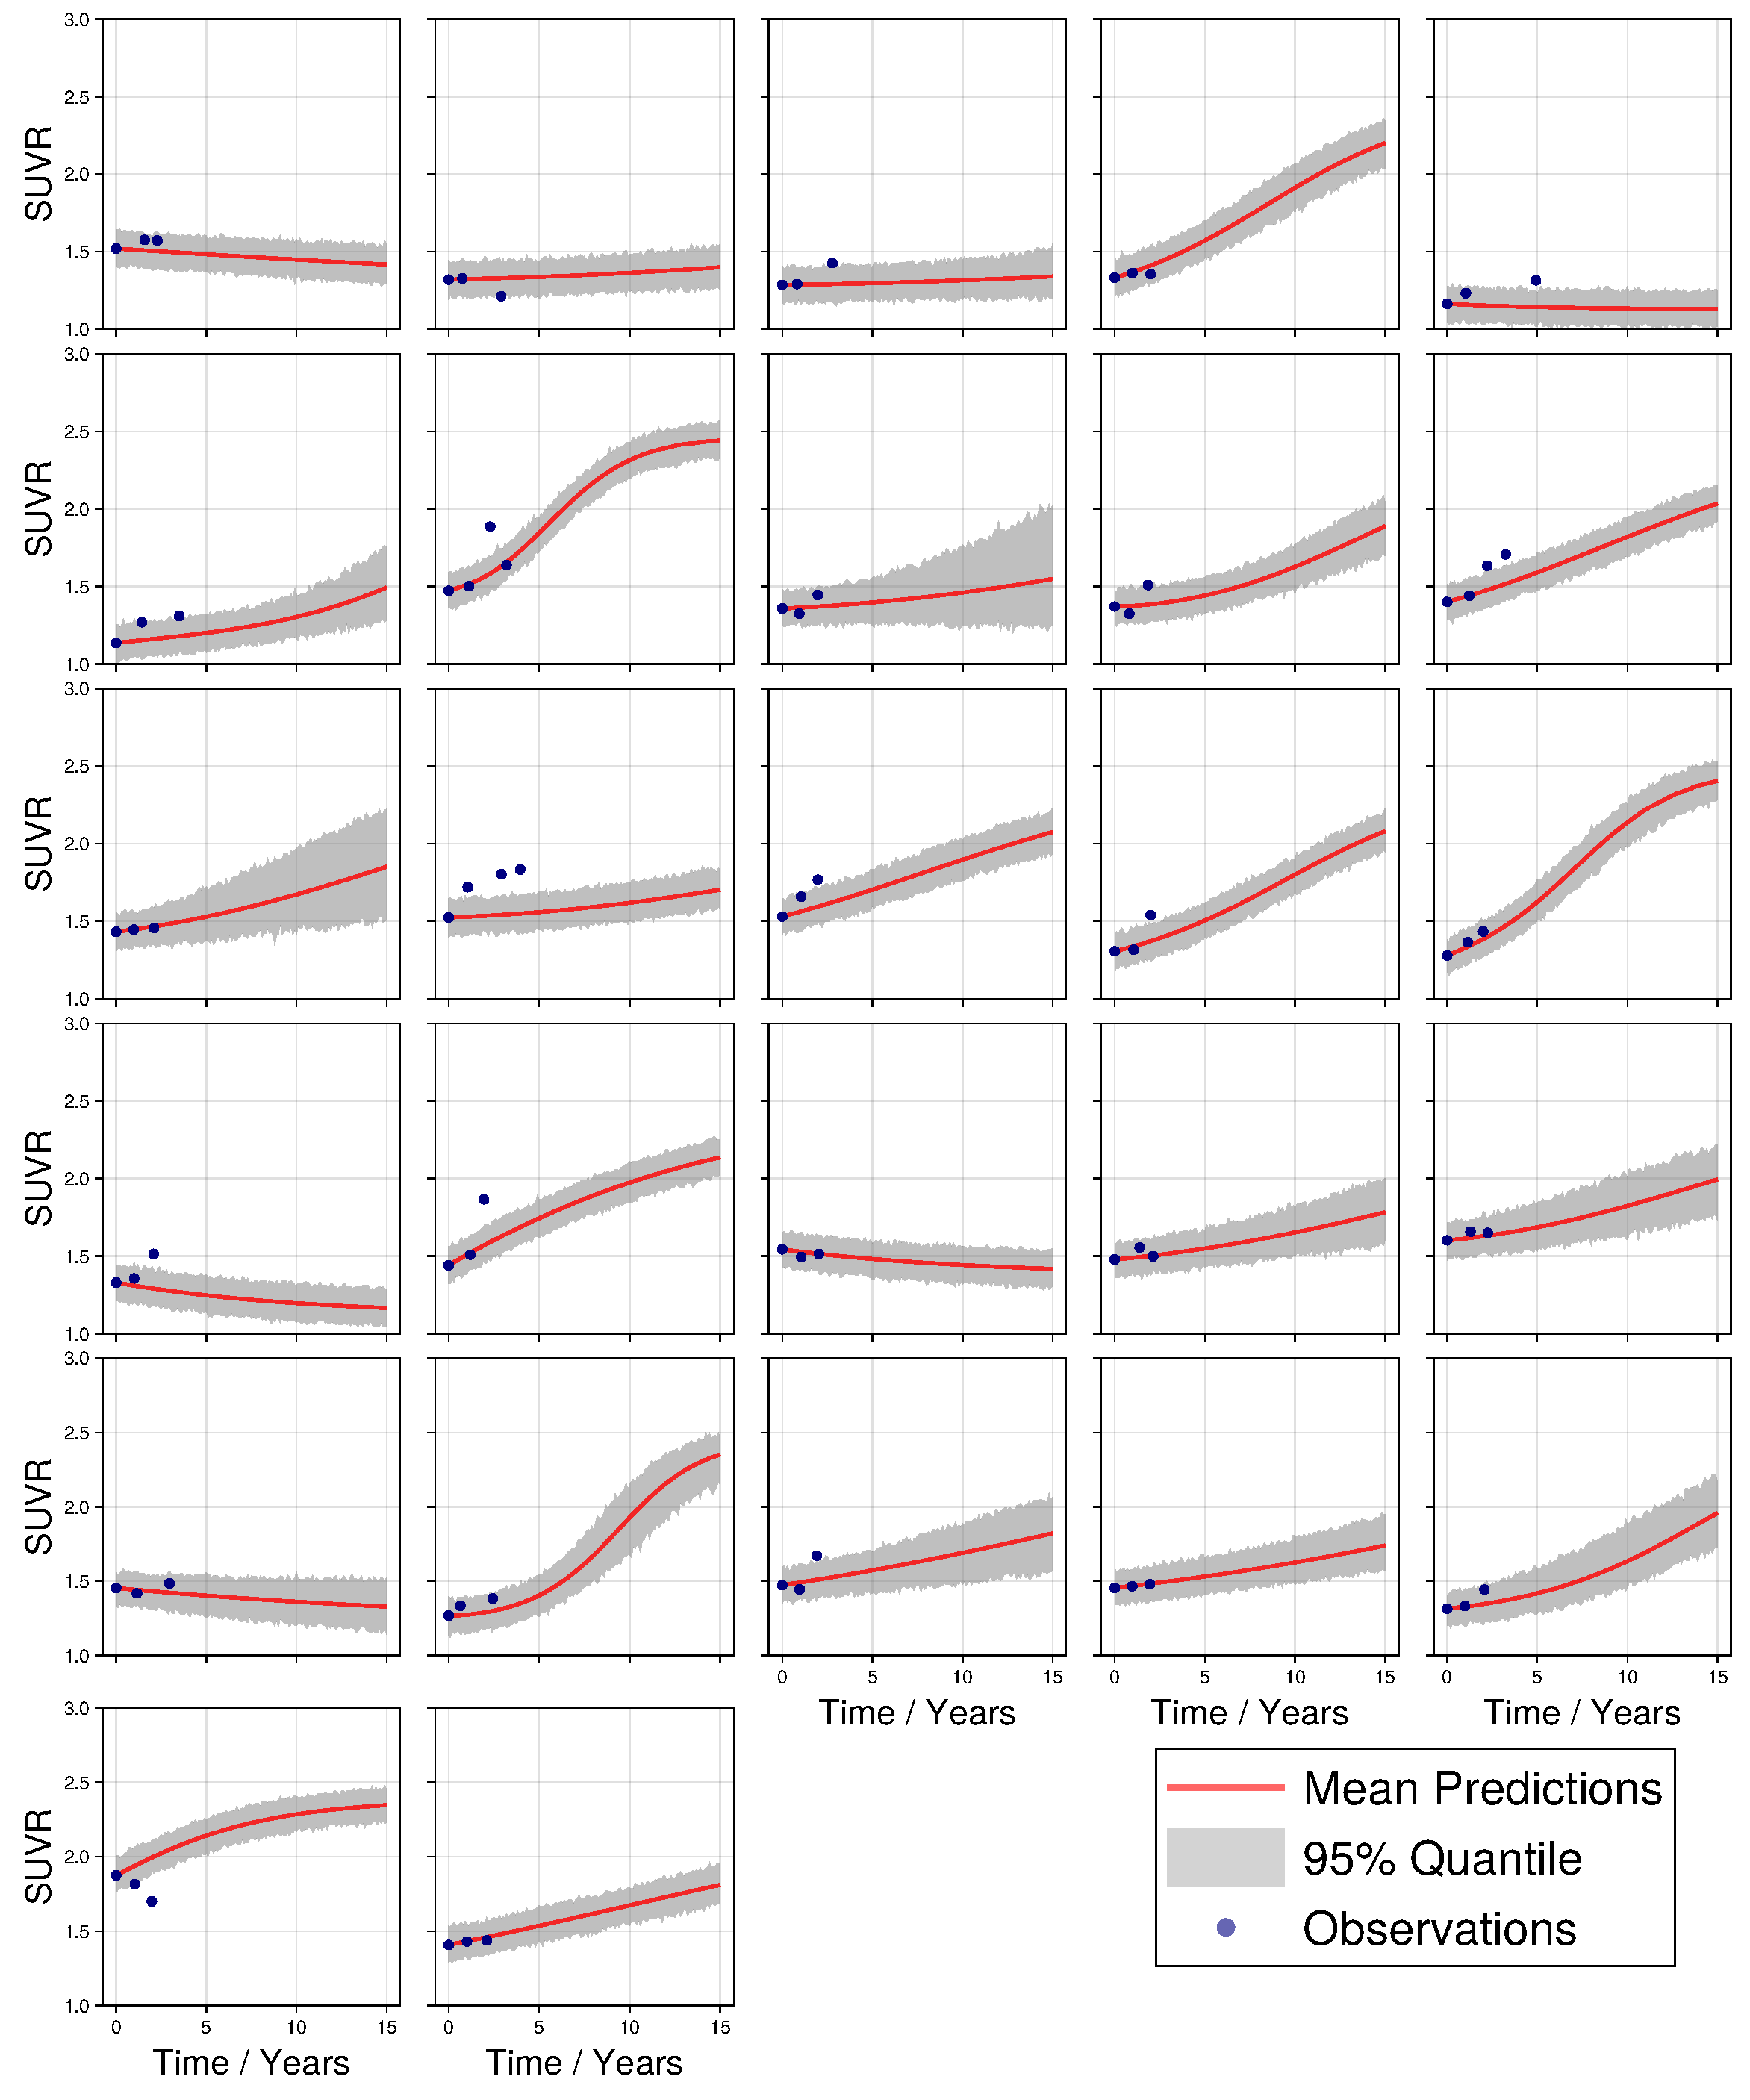
\includegraphics[width=1.0\textwidth]{local-fkpp/inference/pstpred-taupos-entorhinal.pdf}
    \caption{\textbf{Posterior predictive trajectories for the right entorhinal
    cortex in ADNI \ABP \TPP}Forward simulations from the posterior
    distributions of the \TPP group. Shown here are data (blue scatter points)
    and simulated trajectories (mean predictions in red and 95\% confidence
    intervals in grey) from the right entorhinal cortex.}
    \label{fig:pstpred-taupos-ec}
\end{figure}

\begin{figure}[H]
    \centering
    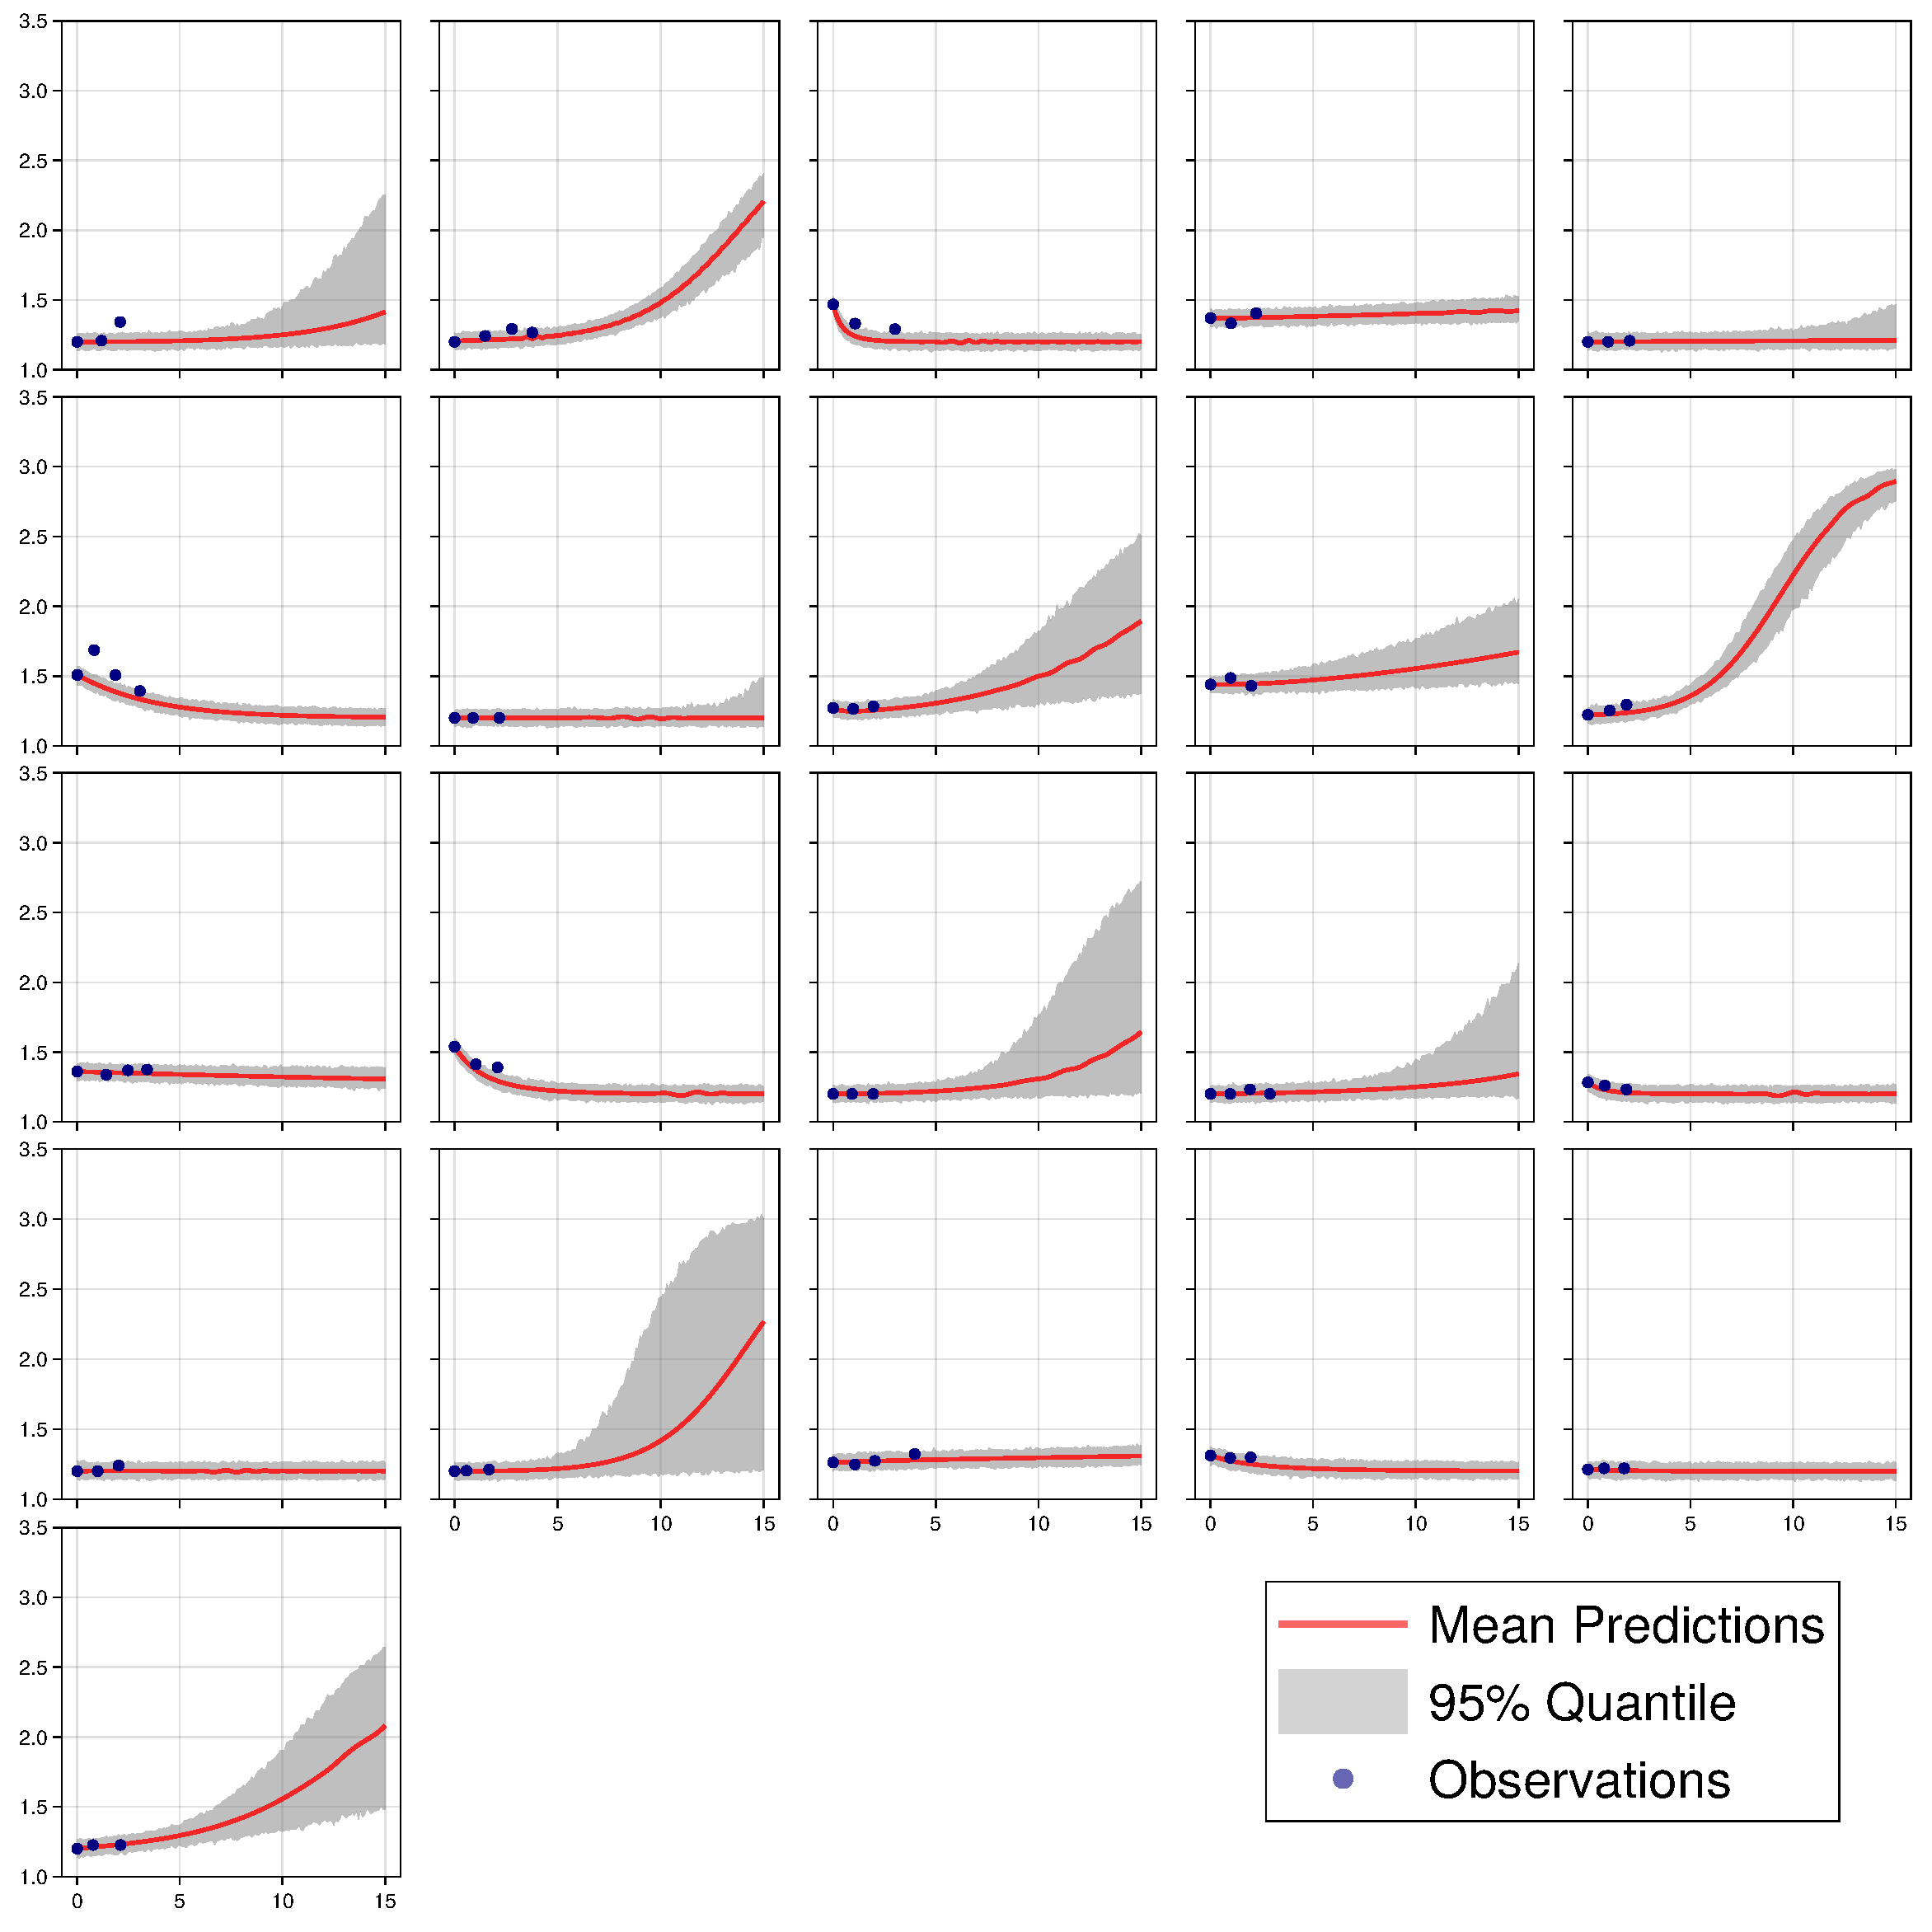
\includegraphics[width=1.0\textwidth]{local-fkpp/inference/pstpred-tauneg-inferiortemporal.pdf}
    \caption{\textbf{Posterior predictive trajectories for the right inferior
    temporal lobe in ADNI \ABP \TPN}Forward simulations from the posterior
    distributions of the \TPN group. Shown here are data (blue scatter points)
    and simulated trajectories (mean predictions in red and 95\% confidence
    intervals in grey) from the right inferior temporal lobe.}
    \label{fig:pstpred-tauneg-it}
\end{figure}

\begin{figure}[H]
    \centering
    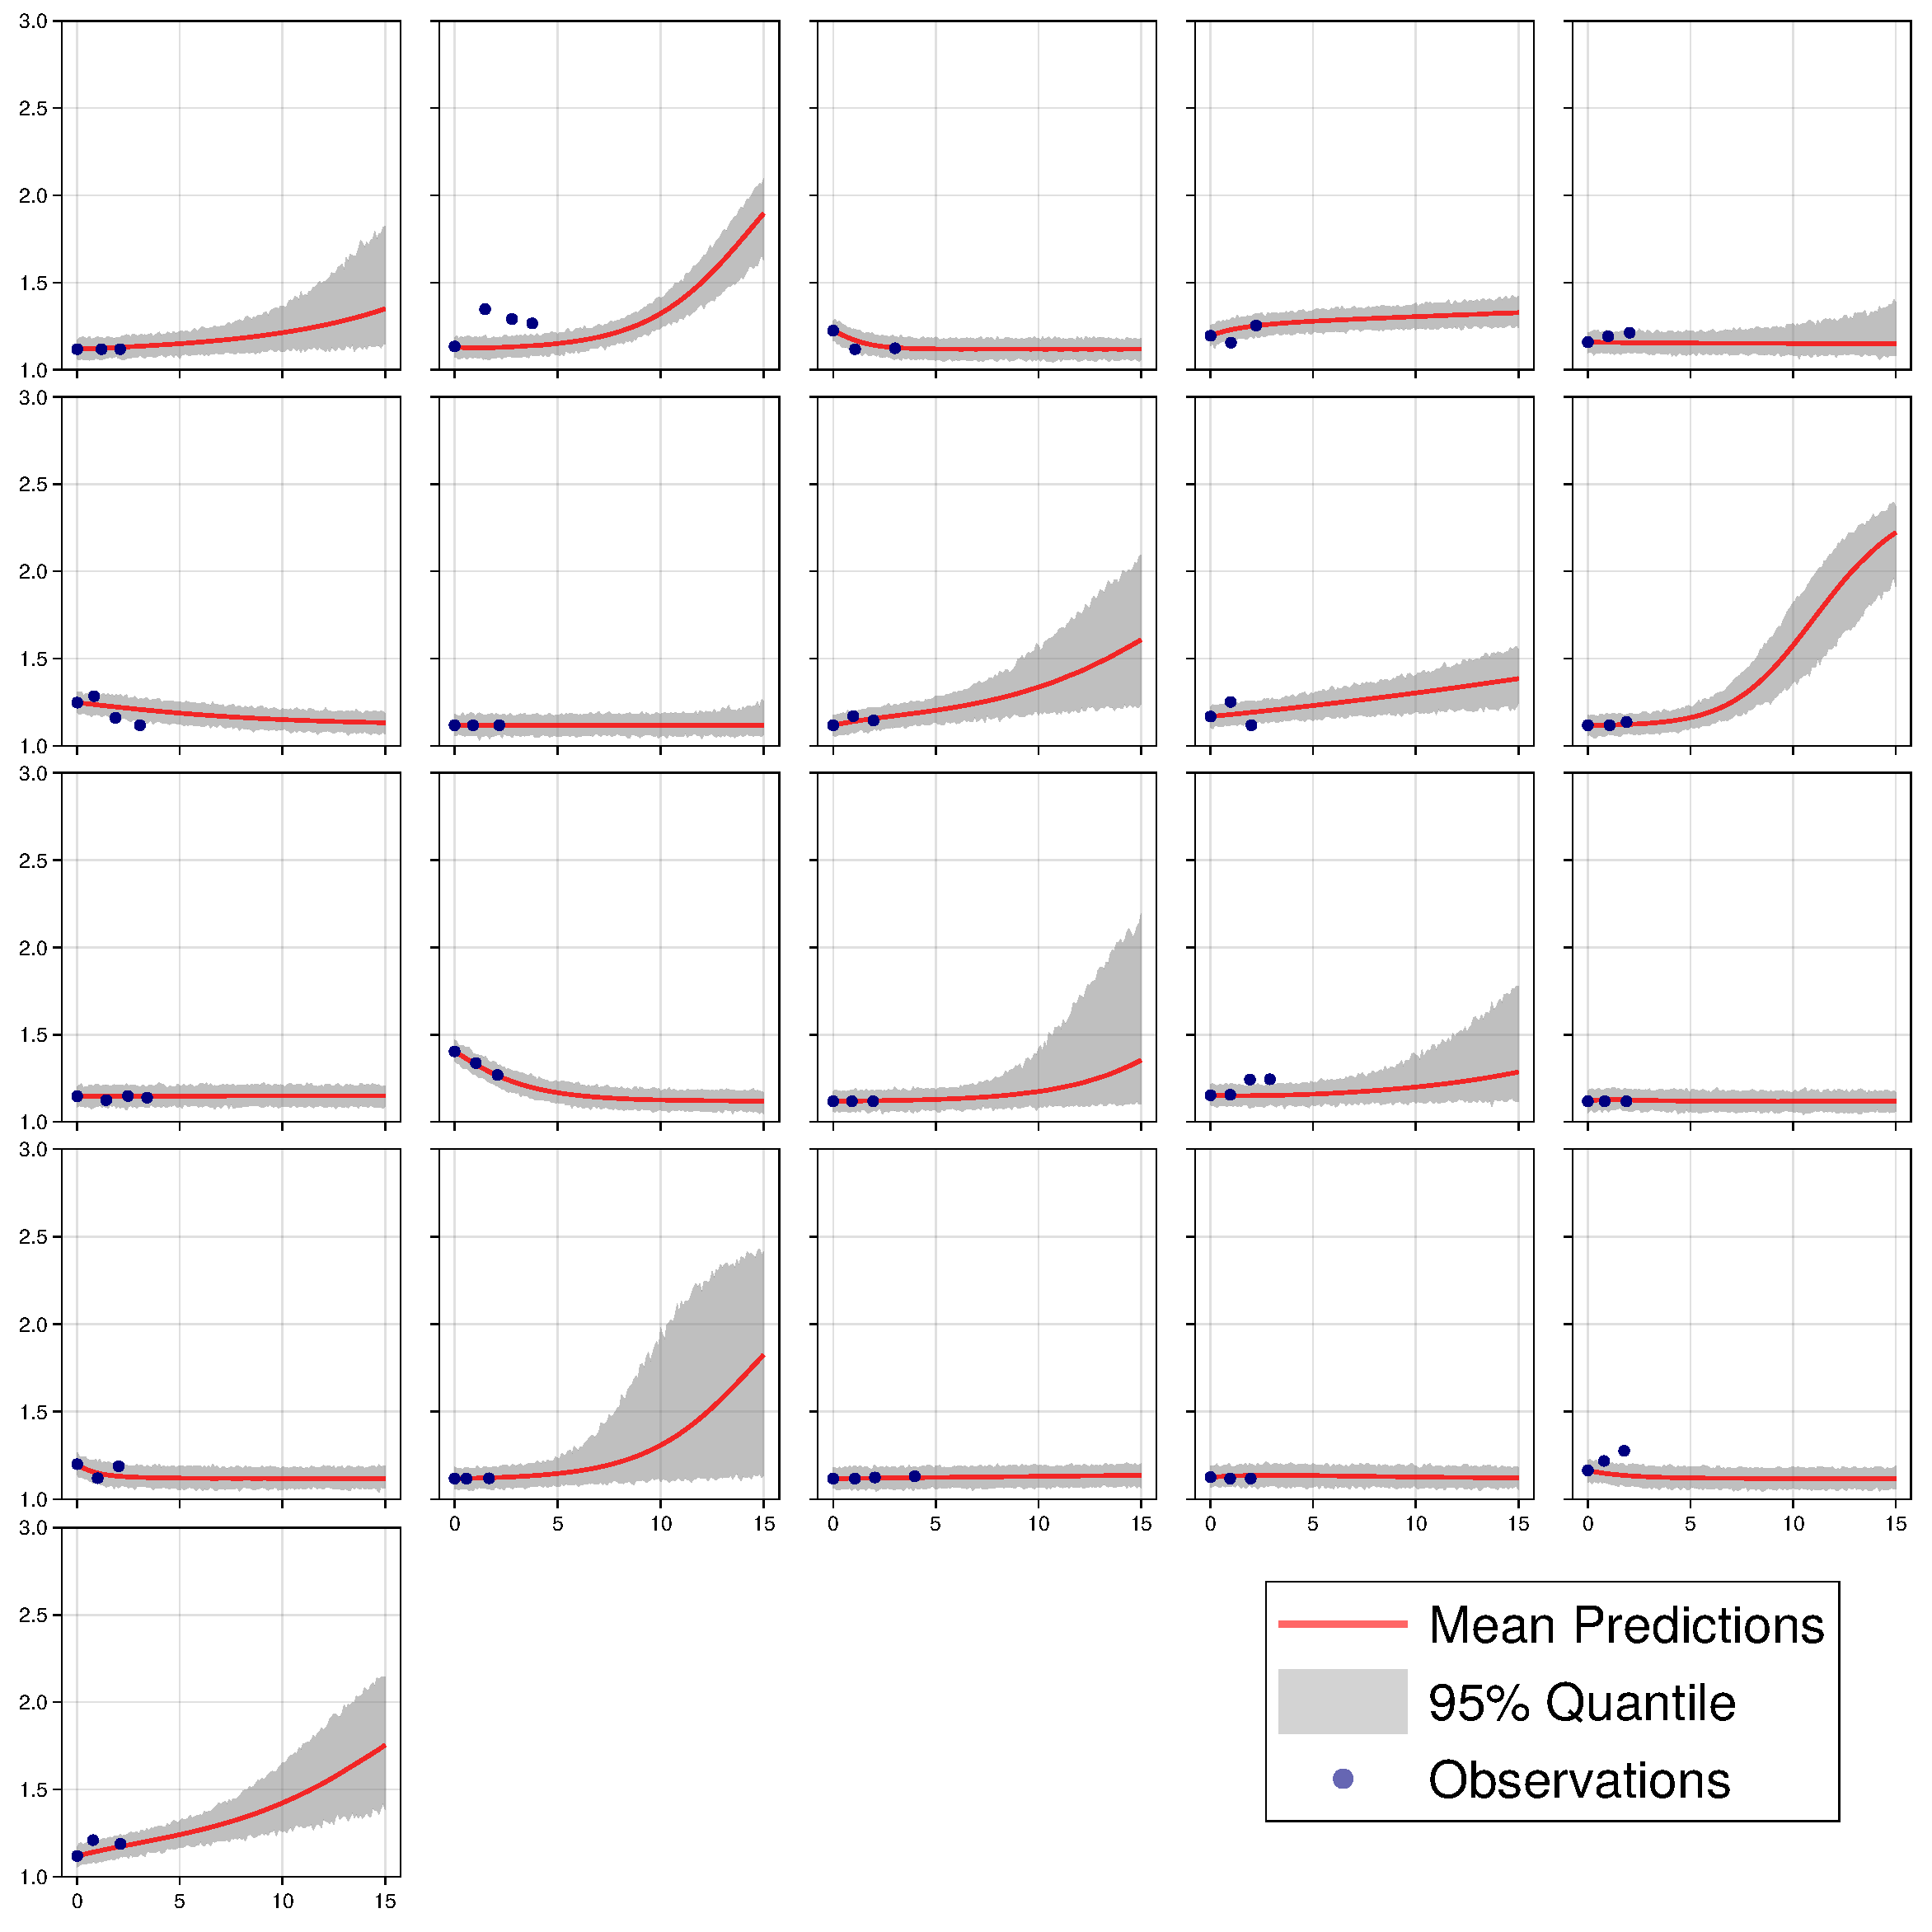
\includegraphics[width=1.0\textwidth]{local-fkpp/inference/pstpred-tauneg-entorhinal.pdf}
    \caption{\textbf{Posterior predictive trajectories for the right entorhinal
    cortex in ADNI \ABP \TPN}Forward simulations from the posterior
    distributions of the \TPN group. Shown here are data (blue scatter points)
    and simulated trajectories (mean predictions in red and 95\% confidence
    intervals in grey) from the right entorhinal cortex.}
    \label{fig:pstpred-tauneg-ec}
\end{figure}


\begin{figure}[H]
    \centering
    \begin{subfigure}{1.0\textwidth}
        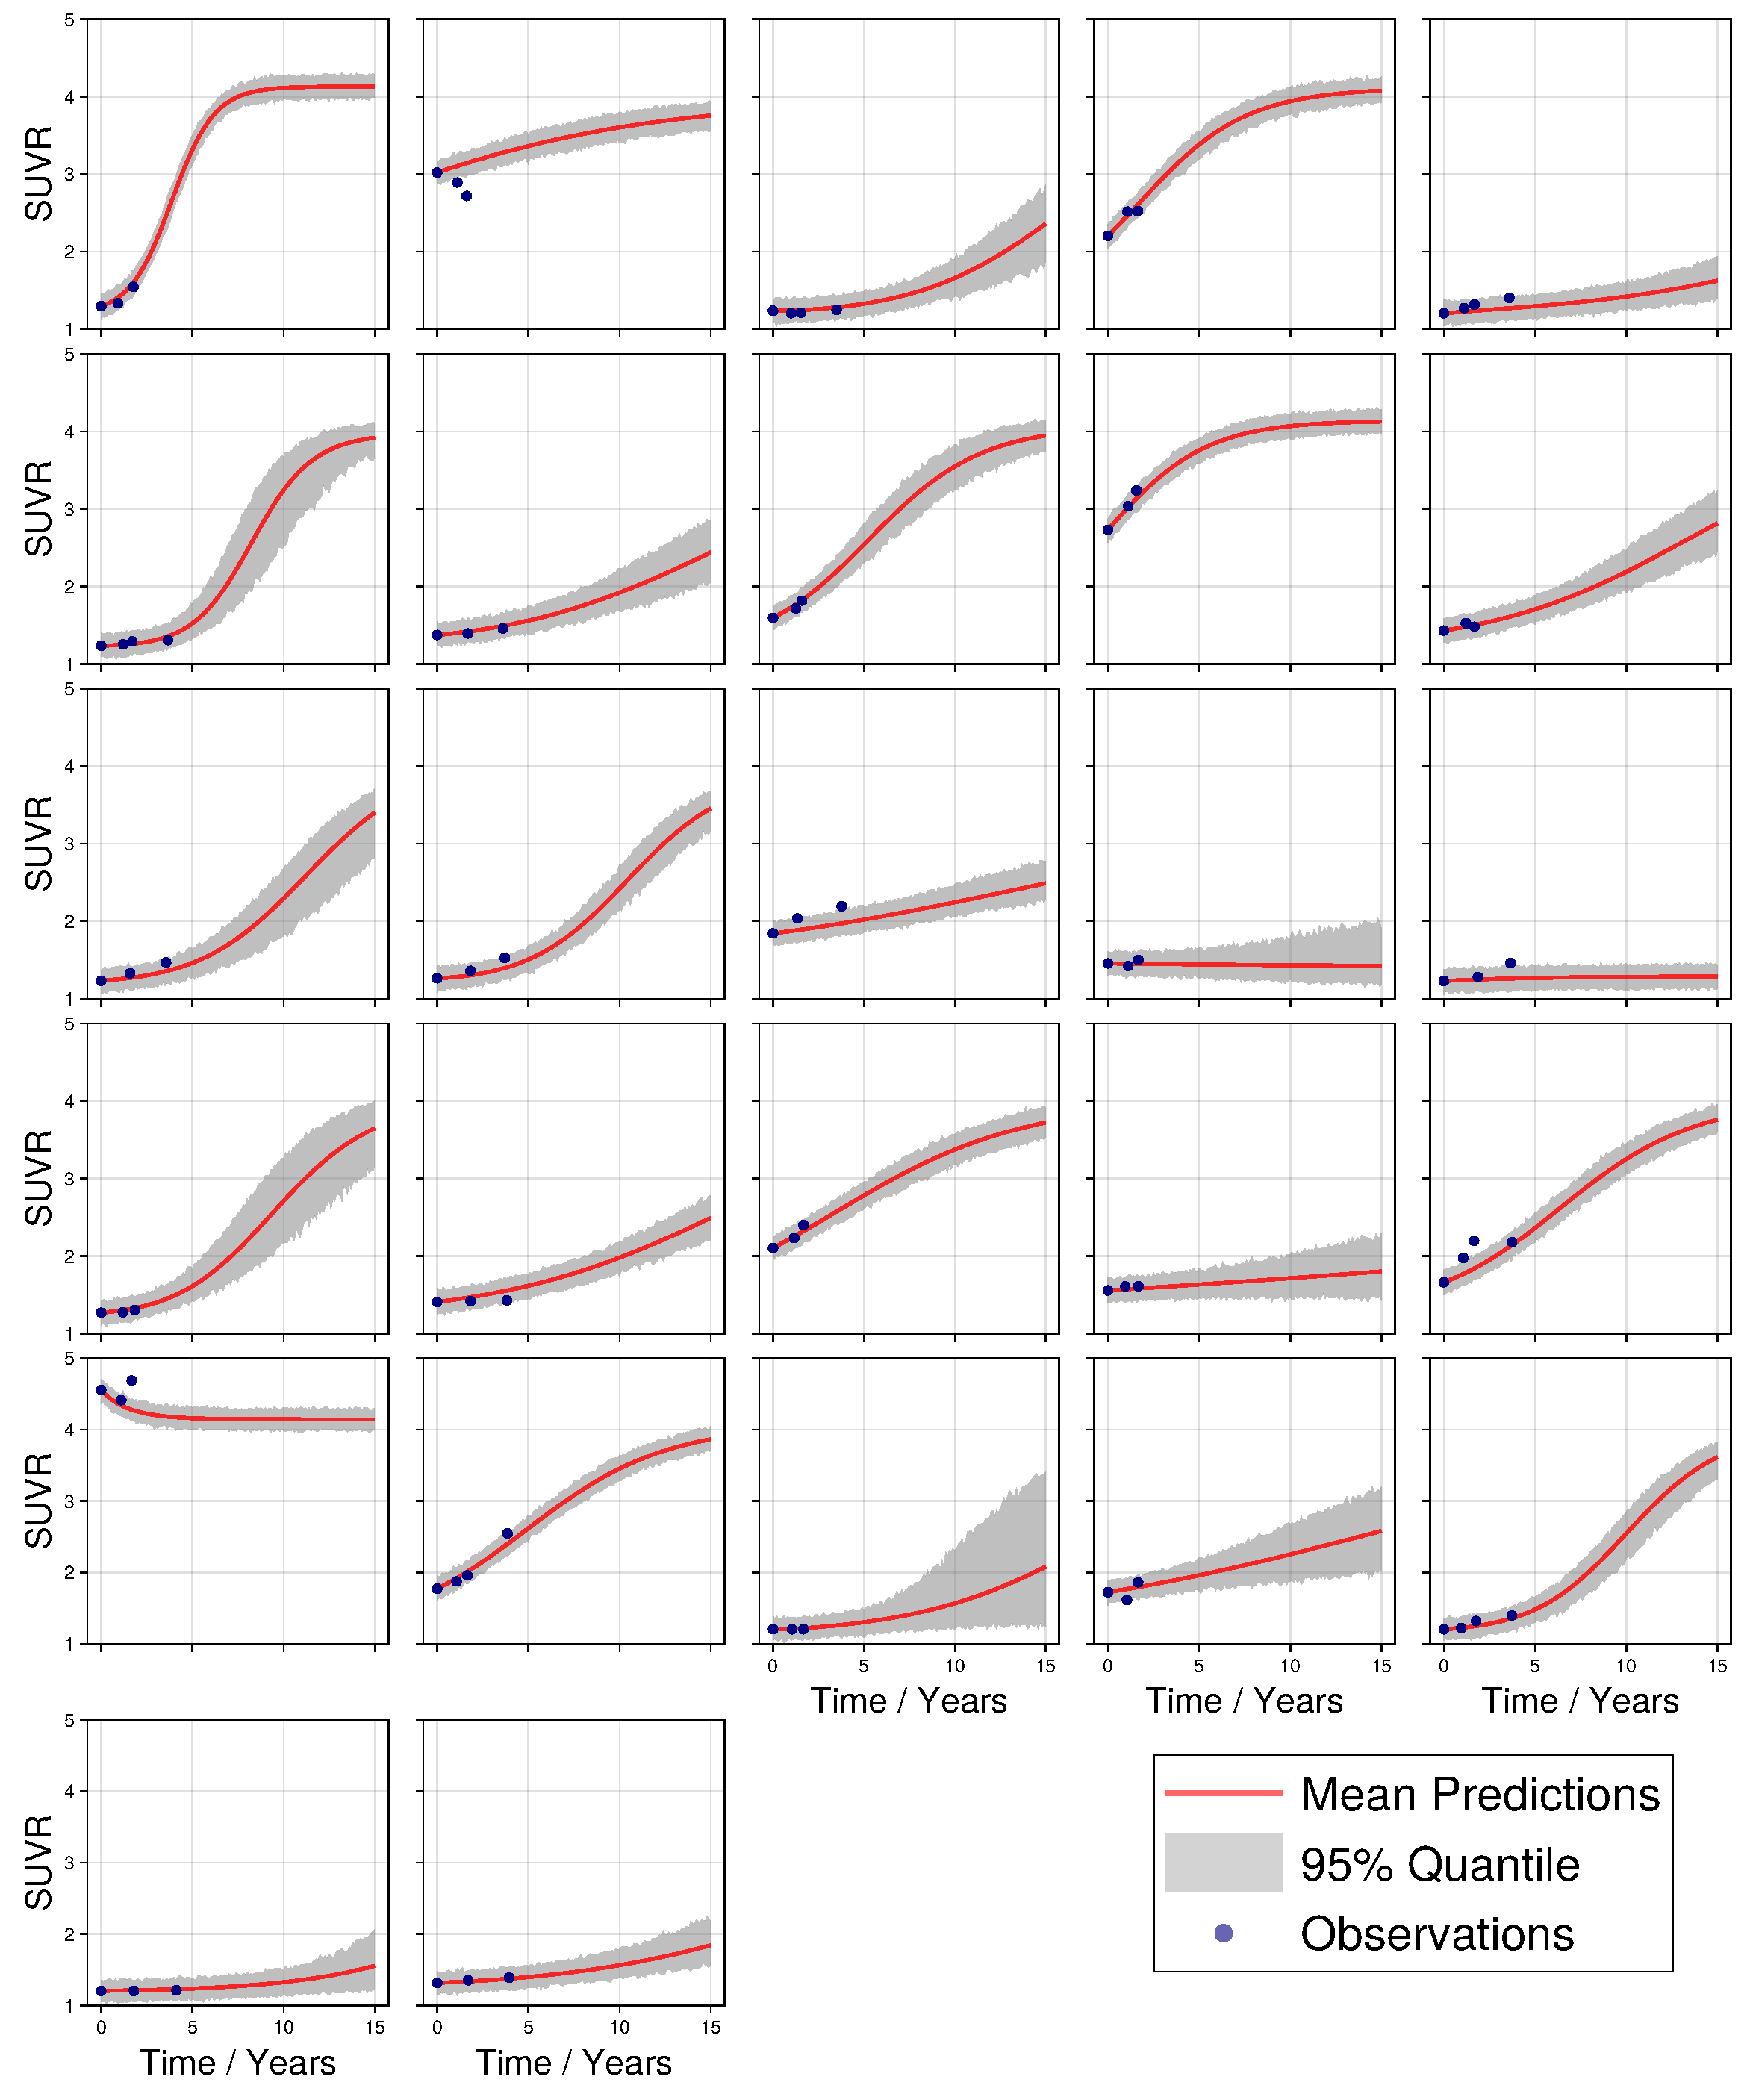
\includegraphics[width=1.0\textwidth]{biofinder/pstpred-taupos-1-inferiortemporal.pdf}
        \label{fig:pstpred-taupos-it-1-bf}
    \end{subfigure} 
    \medskip
    \caption{\textbf{Posterior predictive trajectories for the right 
                     inferior temporal lobe in BF2 \ABP \TPP}.}
\end{figure}%
\begin{figure}[H]\ContinuedFloat
    \centering
    \begin{subfigure}{1.0\textwidth}
        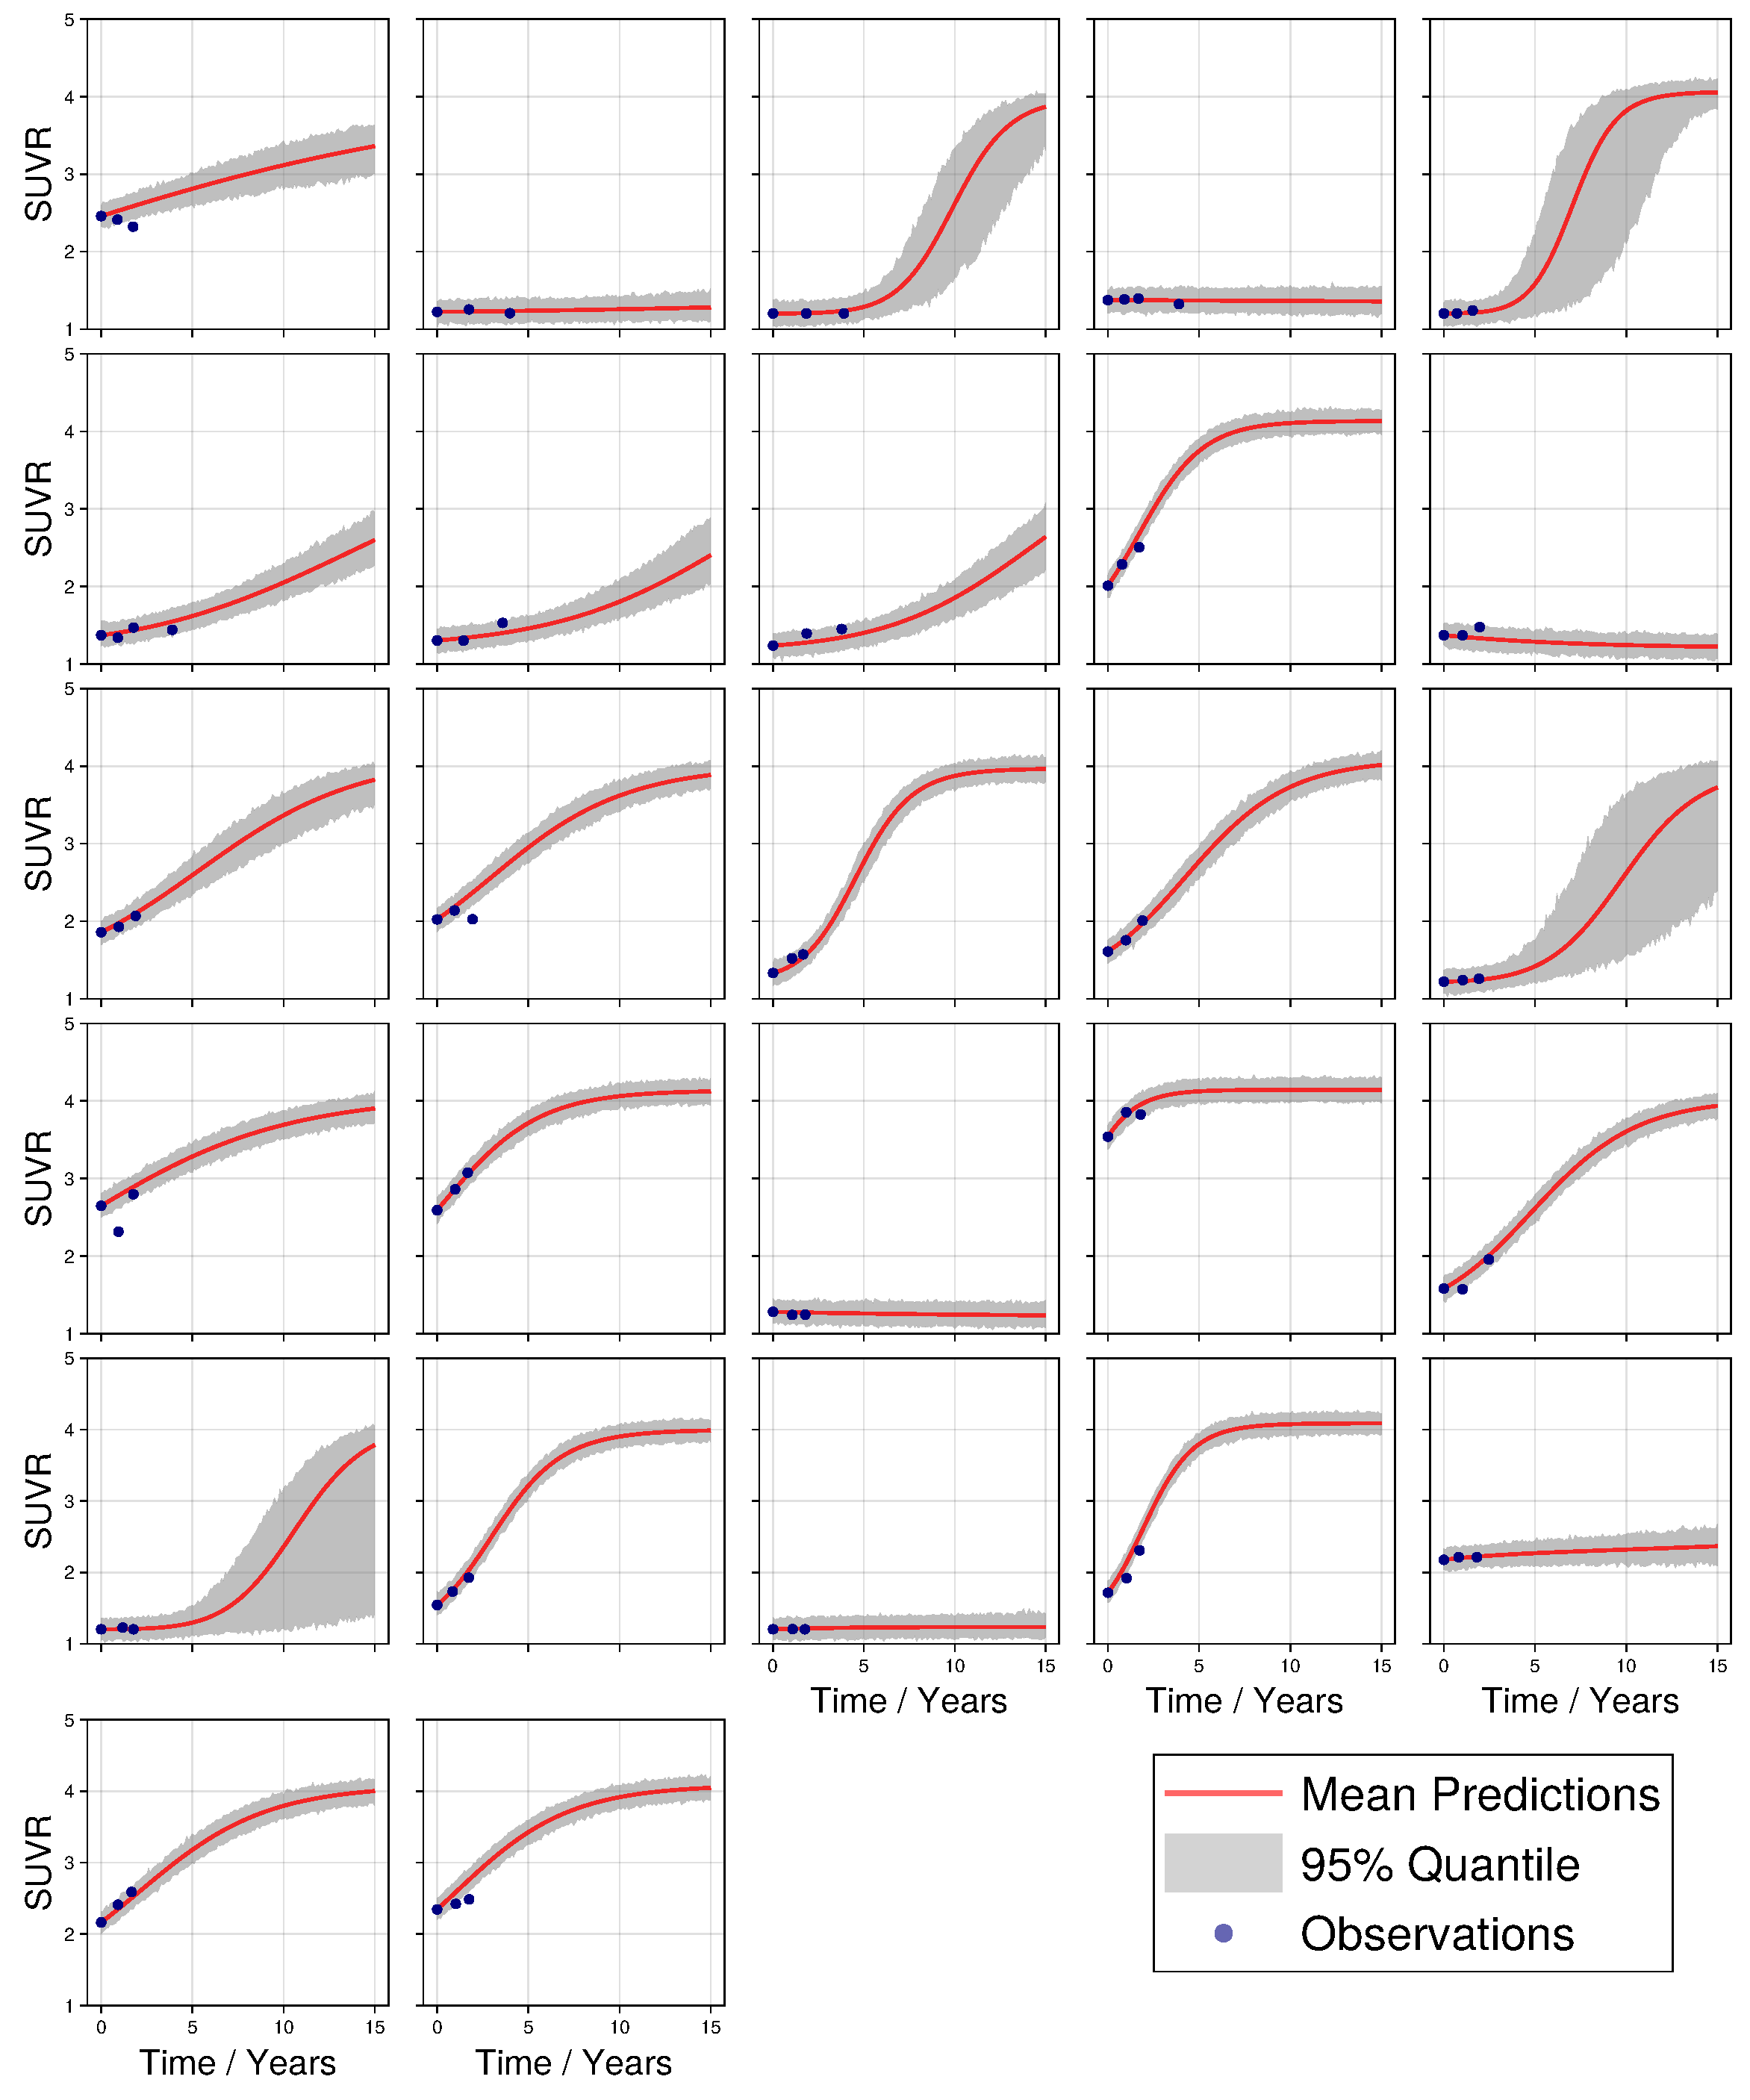
\includegraphics[width=1.0\textwidth]{biofinder/pstpred-taupos-2-inferiortemporal.pdf}
        \label{fig:pstpred-taupos-it-2-bf}
    \end{subfigure}
    \caption[]{\textbf{Posterior predictive trajectories for the right
                       inferior temporal lobe in BF2 \ABP \TPP (cont.)}
    Simulations from the posterior distributions of the BF2
    \ABP \TPP group. Shown here are data (blue scatter points) and simulated 
    trajectories (mean predictions in red and 95\% confidence intervals in grey)
    from the right inferior temporal lobe}
    \label{fig:pstpred-taupos-it-bf}
\end{figure}

\begin{figure}[H]
    \centering
    \begin{subfigure}{1.0\textwidth}
        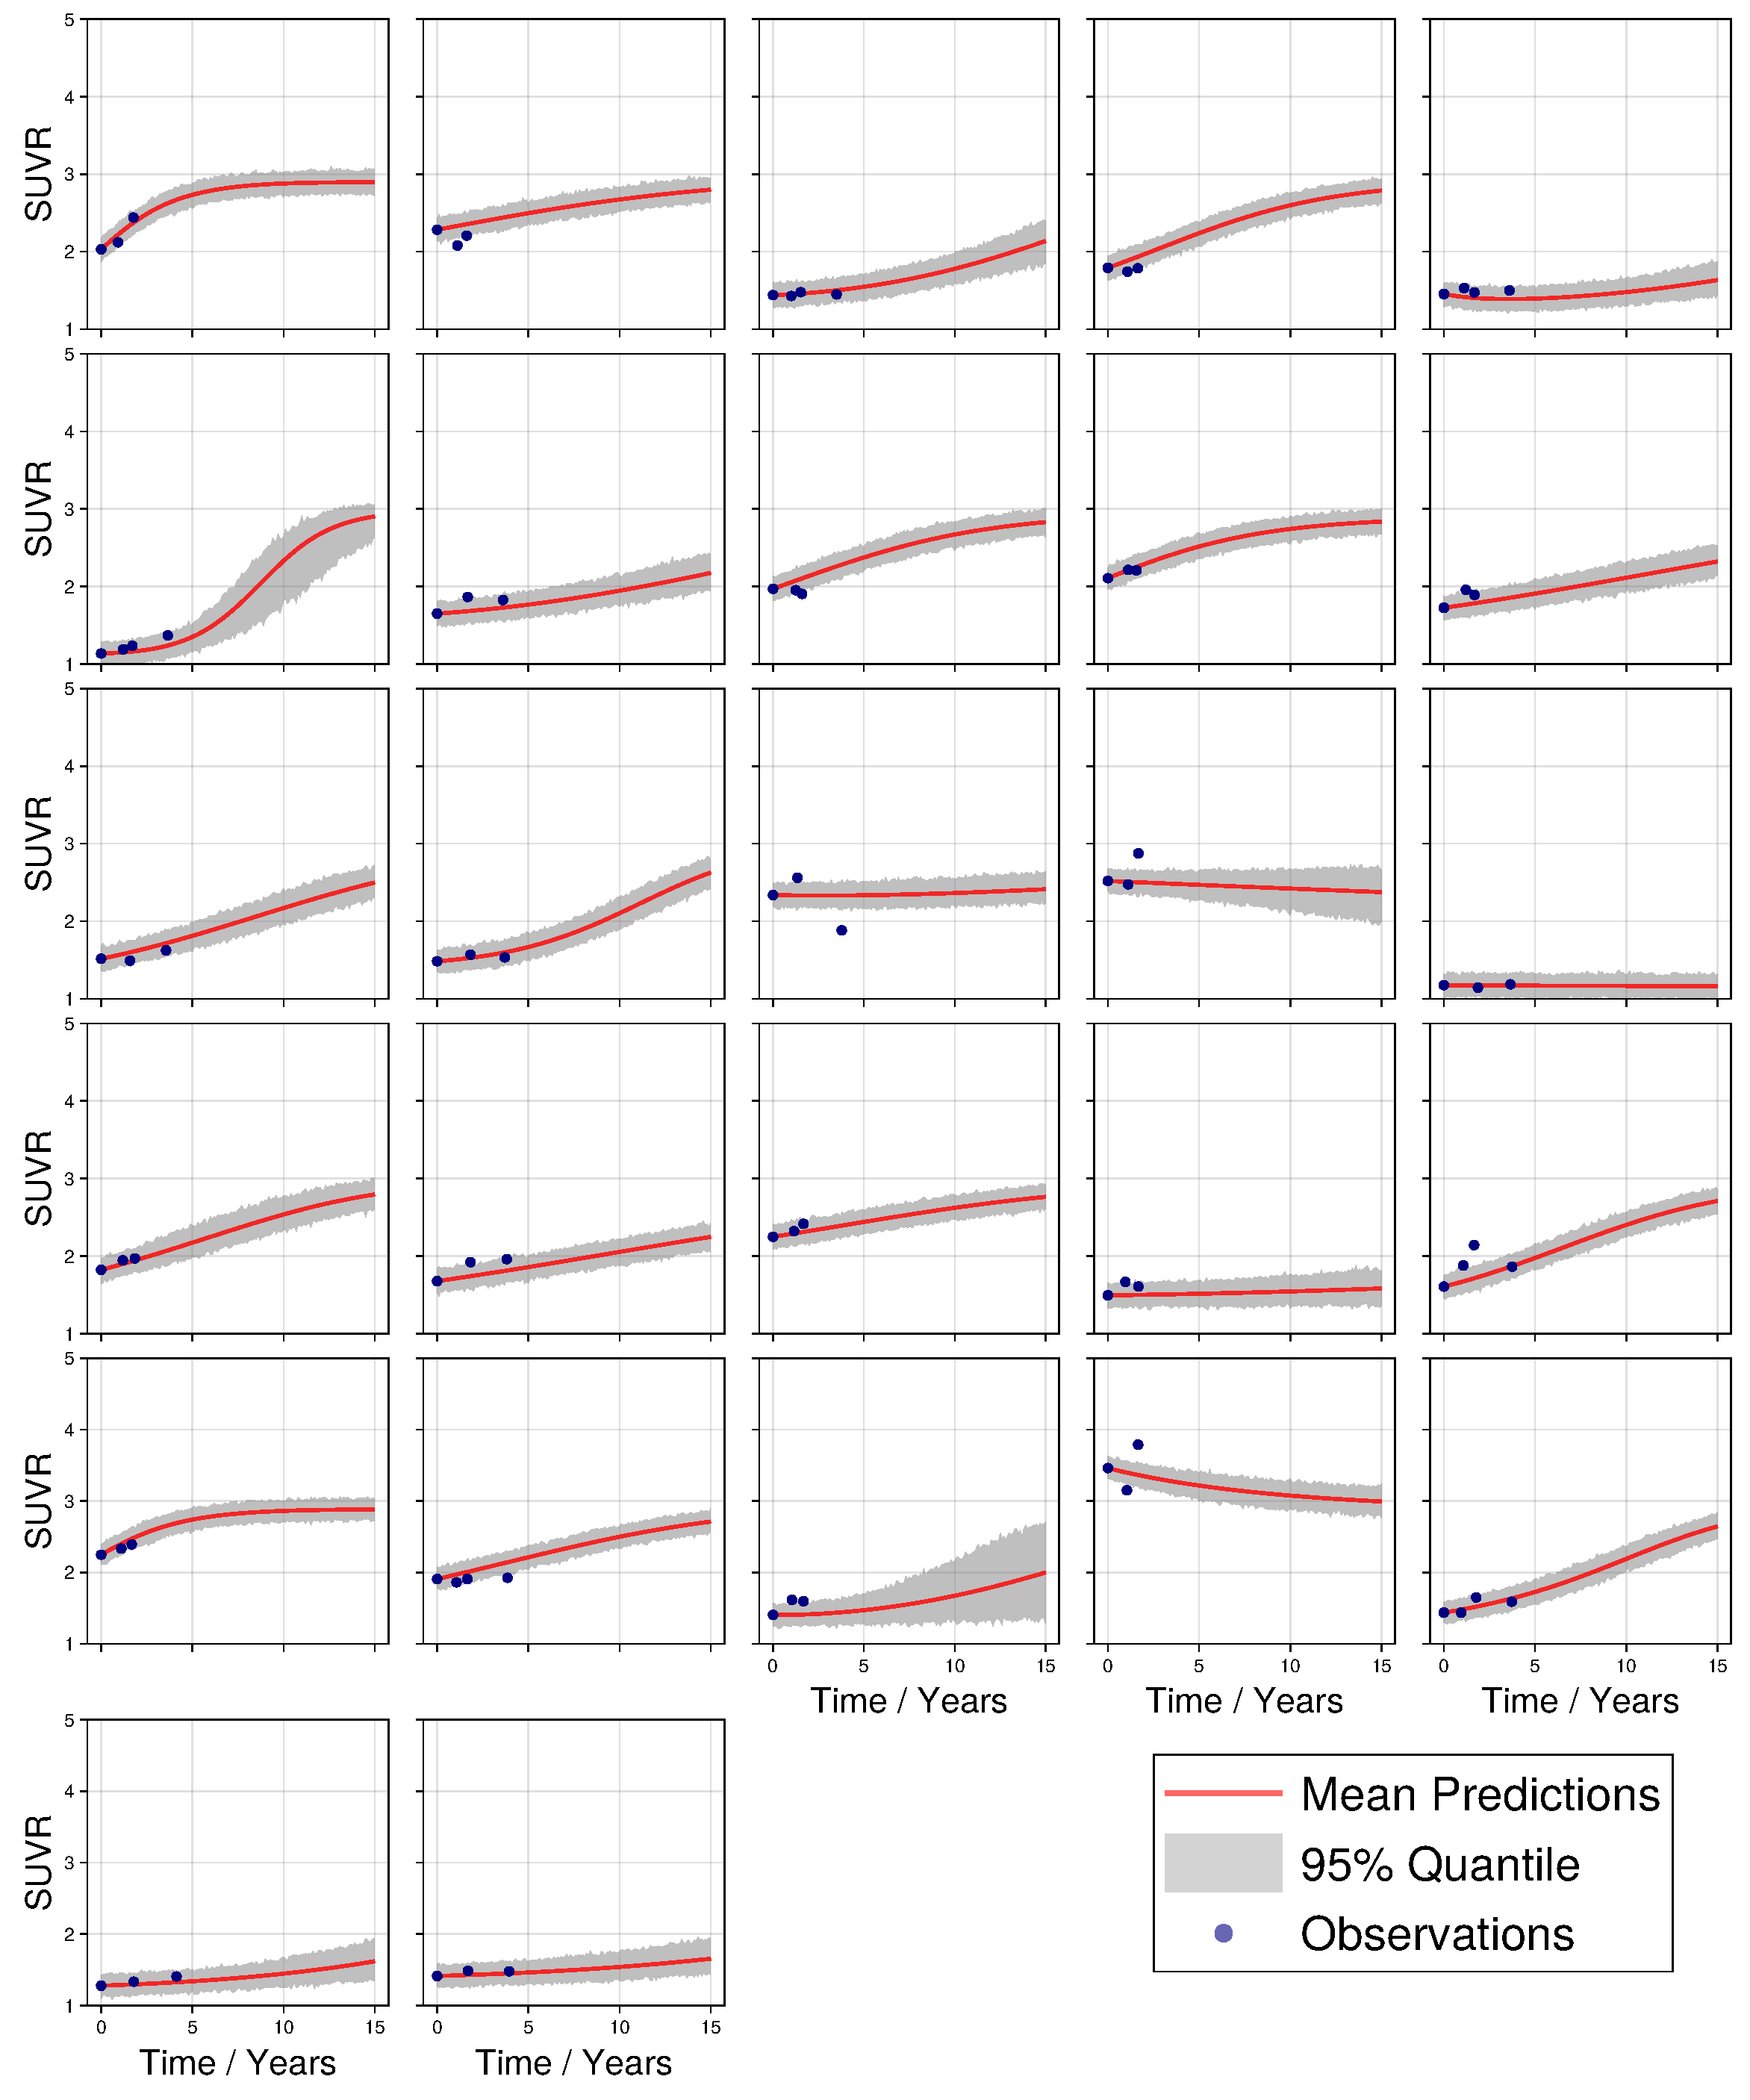
\includegraphics[width=1.0\textwidth]{biofinder/pstpred-taupos-1-entorhinal.pdf}
        \label{fig:pstpred-taupos-ec-1-bf}
    \end{subfigure} 
    \medskip
    \caption{\textbf{Posterior predictive trajectories for the right
                     entorhinal cortex in BF2 \ABP \TPP}.}
\end{figure}%
\begin{figure}[H]\ContinuedFloat
    \centering
    \begin{subfigure}{1.0\textwidth}
        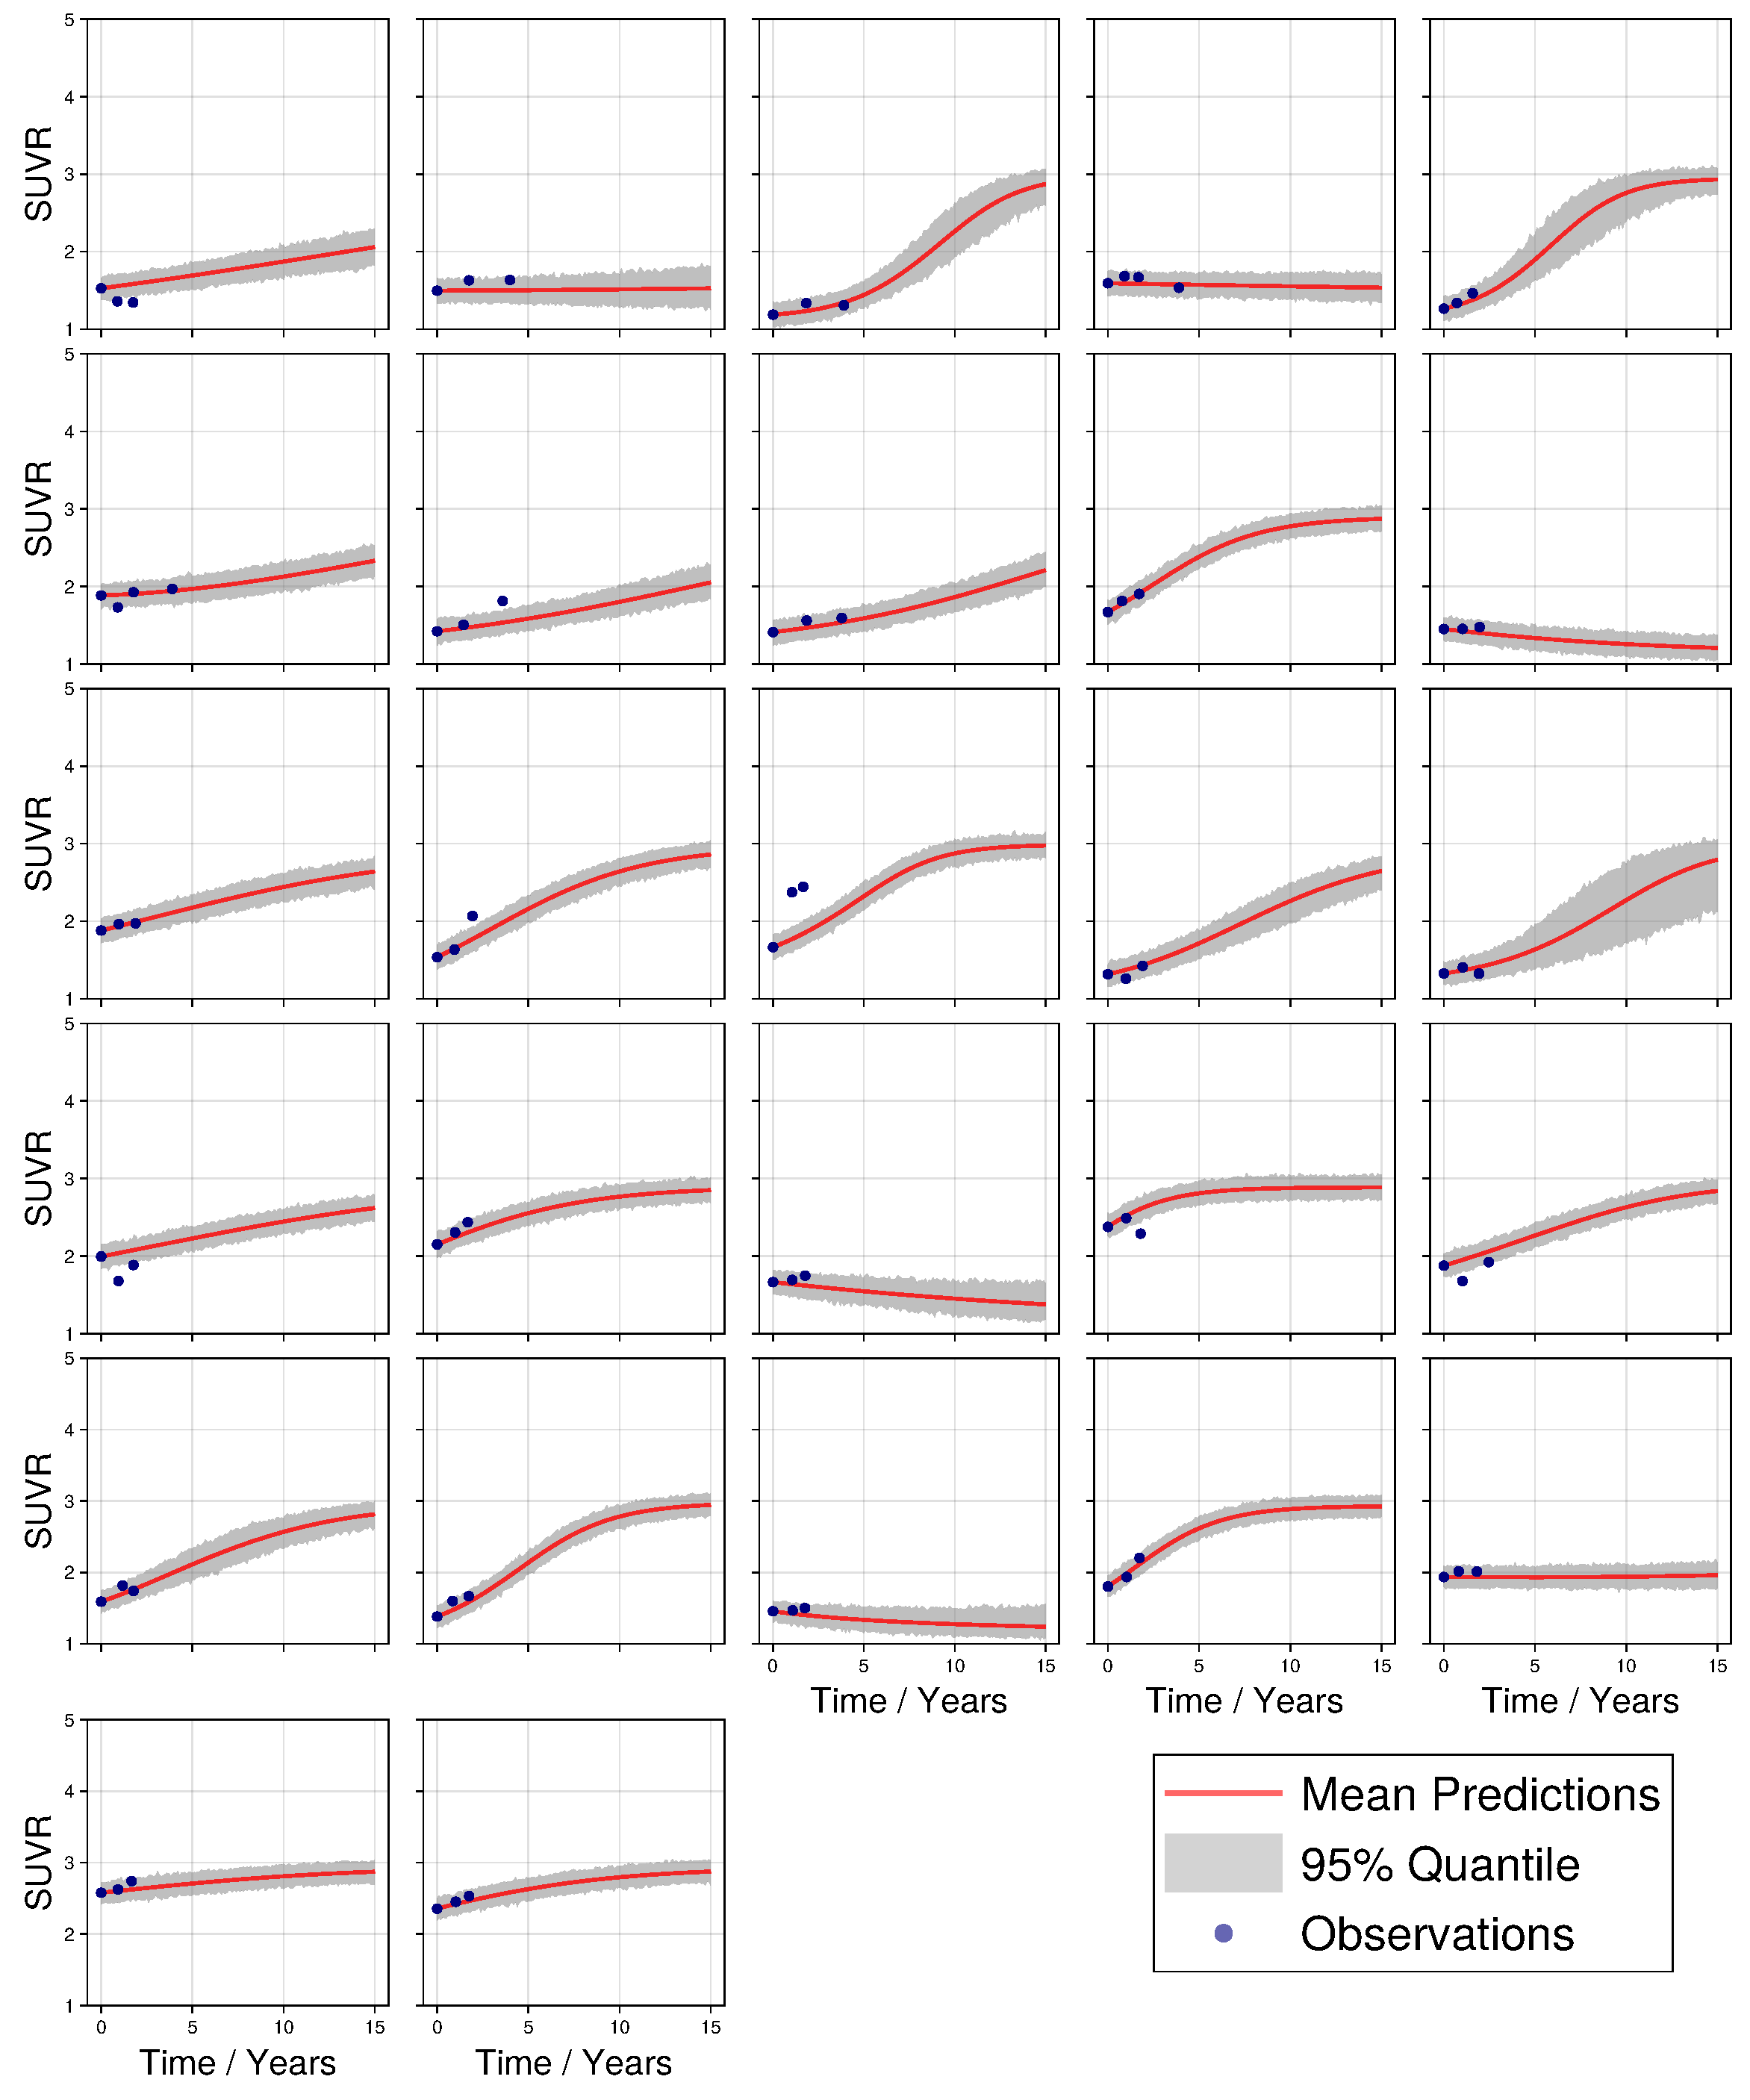
\includegraphics[width=1.0\textwidth]{biofinder/pstpred-taupos-2-entorhinal.pdf}
        \label{fig:pstpred-taupos-ec-2-bf}
    \end{subfigure}
    \caption[]{\textbf{Posterior predictive trajectories for the right
                       entorhinal cortex in BF2 \ABP \TPP (cont.)}
    Simulations from the posterior distributions of the BF2
    \ABP \TPP group. Shown here are data (blue scatter points) and simulated 
    trajectories (mean predictions in red and 95\% confidence intervals in grey)
    from the right entorhinal cortex}
    \label{fig:pstpred-taupos-ec-bf}
\end{figure}


\begin{figure}[H]
    \centering
    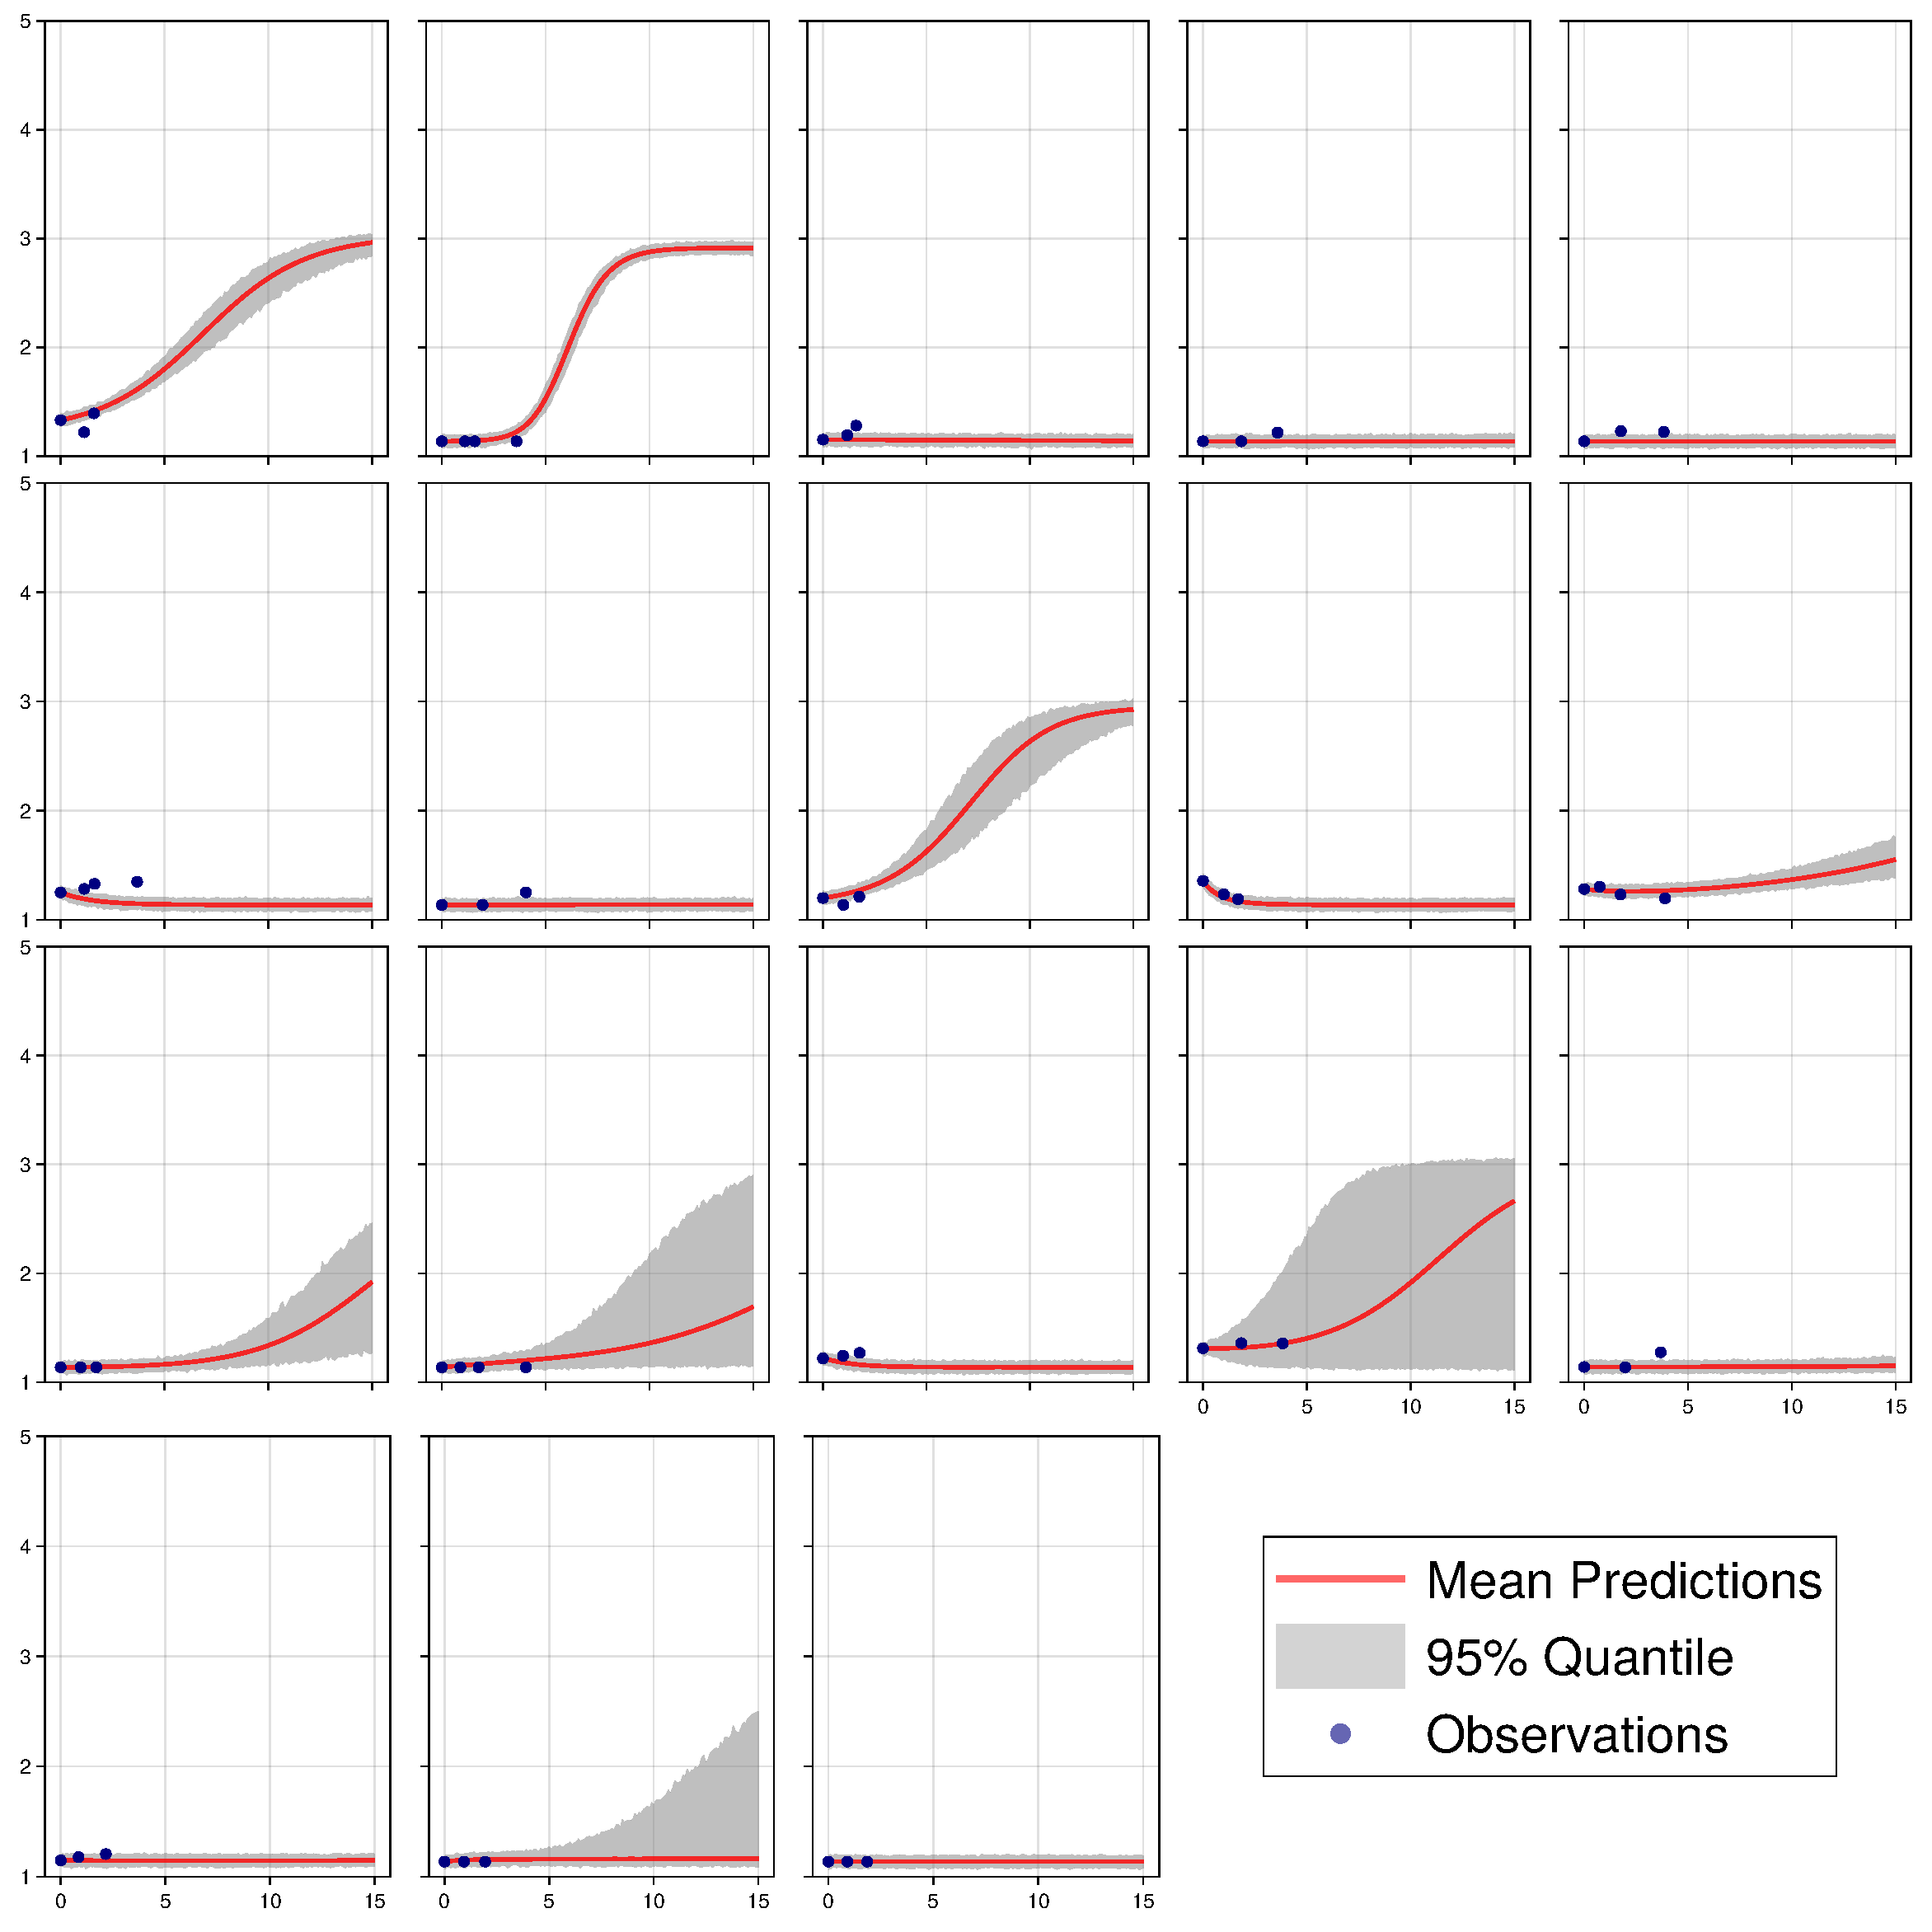
\includegraphics[width=1.0\textwidth]{biofinder/pstpred-tauneg-entorhinal.pdf}
    \caption{\textbf{Posterior predictive trajectories for the right
                     entorhinal cortex in BF2 \ABP \TPN}.
    Simulations from the posterior distributions of the BF2
    \ABP \TPN group. Shown here are data (blue scatter points) and simulated 
    trajectories (mean predictions in red and 95\% confidence intervals in grey)
    from the right entorhinal cortex}
    \label{fig:pstpred-tauneg-ec-bf}
\end{figure}

\begin{figure}[H]
    \centering
    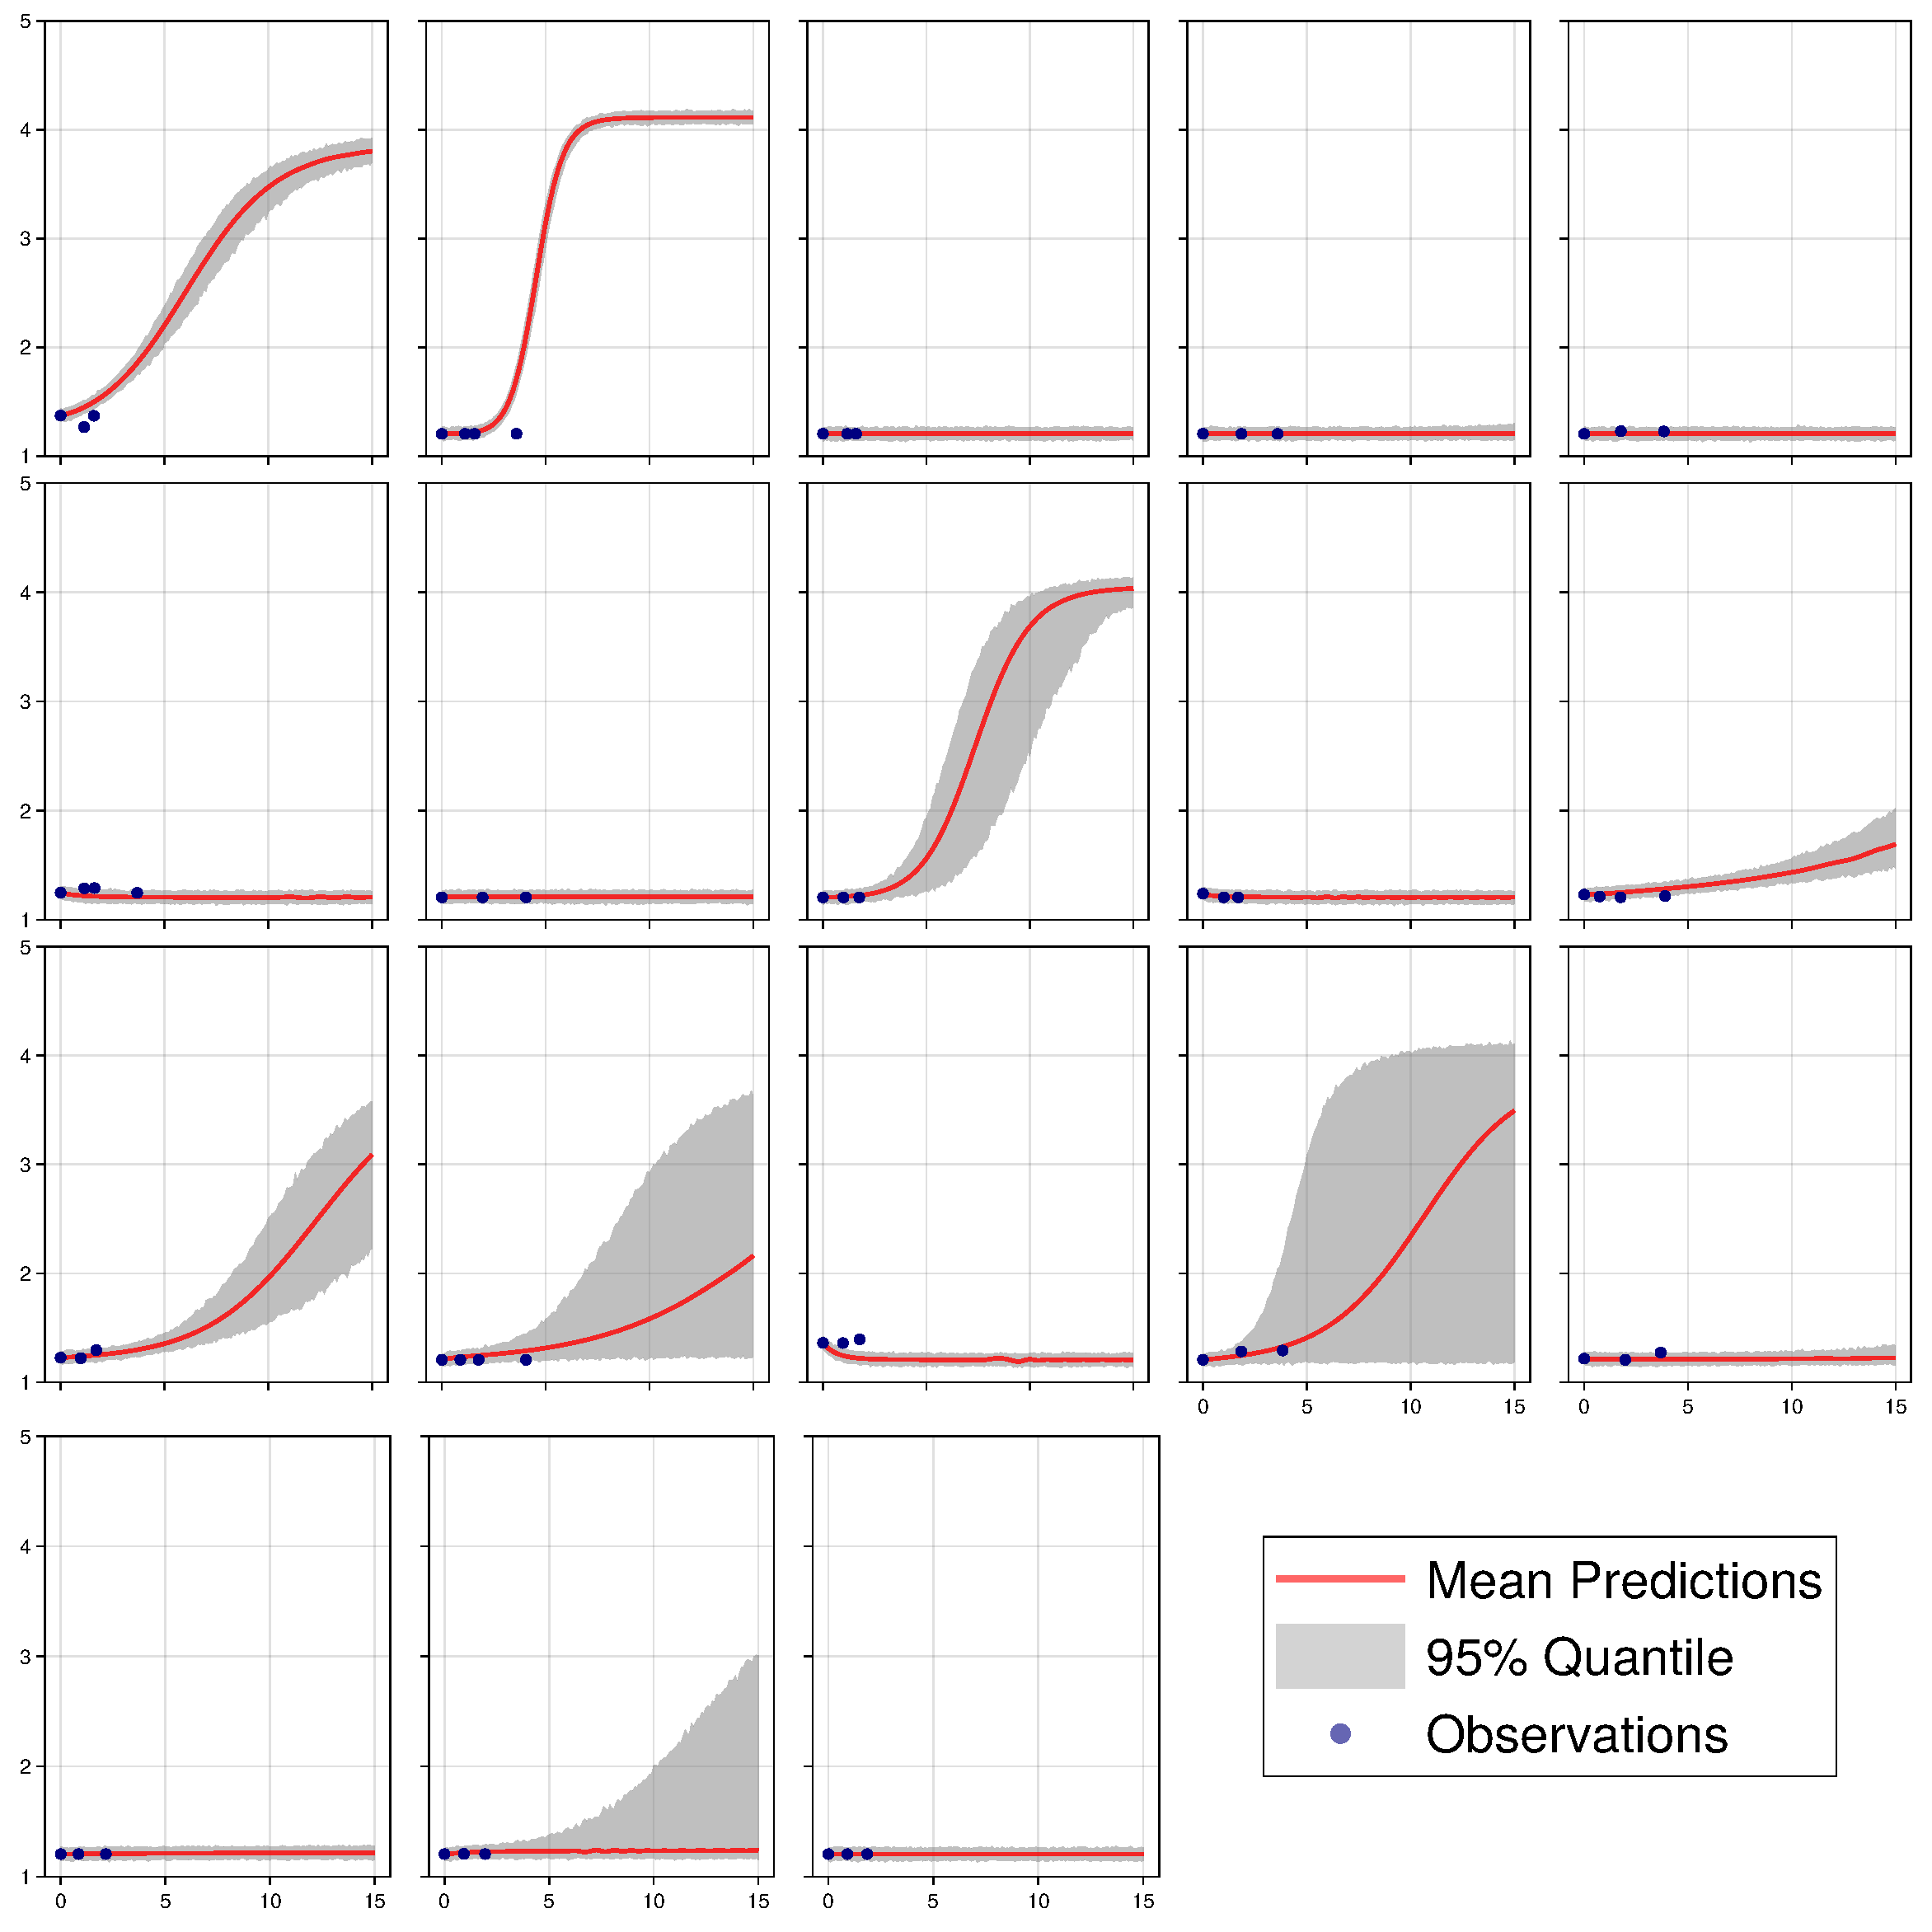
\includegraphics[width=1.0\textwidth]{biofinder/pstpred-tauneg-inferiortemporal.pdf}
    \caption{\textbf{Posterior predictive trajectories for the right
                     inferior temporal lobe in BF2 \ABP \TPN}.
    Simulations from the posterior distributions of the BF2
    \ABP \TPN group. Shown here are data (blue scatter points) and simulated 
    trajectories (mean predictions in red and 95\% confidence intervals in grey)
    from the right inferiortemporal lobe}
    \label{fig:pstpred-tauneg-it-bf}
\end{figure}

\section{Discussion and Conclusions}

In this chapter, I have shown how a Bayesian framework can be used to fit a model
of \TP pathology to \TP PET data obtained from subjects across the AD spectrum.
By performing inference across different patient
groups, we have demonstrated the effects of elevated \AB and \TP levels in
patient groups, showing that subjects who are \ABN have a lower risk of disease
progression, contrasted with the higher risk group \ABP \TPN and even higher
risk \ABP \TPP group.

There have been several studies that use different kinds of computational models
to explain proteopathy in AD \cite{raj2015network, vogel2020spread}. A key
difference among the models presented in the literature are descriptions of
growth processes. For example, the diffusion model presented in
\cite{raj2012network,raj2015network} use only diffusion across the structural
connectome, whereas the epidemic spreading model presented in
\cite{iturria2014epidemic} incorporates regional growth and clearance. In this
paper, we present a parsimonious model of diffusion across the brain network and
regionally specific growth rates that relies on only two free parameters, a
global diffusion coefficient and a global protein growth rate. Using the
Gaussian mixture modelling approach to \TP PET processing presented in
\cite{vogel2020spread}, we are able to determine fixed parameters for regional
baseline values and carrying capacities, which intrinsically inform regional
growth dynamics. Our results demonstrate heterogeneity in regional growth rates,
showing that some regions are more susceptible to tau invasion and
proliferation. Additionally, our model proves to be robustly identifiable from
even limited patient data, capturing almost all variations in data within the
95\% confidence interval. 

The physical basis of the model allows for mechanistic interpretation of our
parameter inference results. Our results are consistent with experimental and
theoretical work purporting the transport of \TP through anatomical connections
\cite{liu2012trans,devos2018synaptic,vogel2020spread}. We further show that
during early stages of disease, when there is a low \TP concentration in the
medial temporal lobe, \TP dynamics are diffusion dominated but become growth
dominated later in disease. This supports previous work by Meisl et al.
\cite{meisl2021vivo} who show through an analysis of multiple datasets and
methods of \TP quantification that \TP dynamics are growth dominated from Braak
stage 3 onwards. Our results also demonstrate the growth rate of \TP increases
with the accumulation of \TP and is accelerated in later stage AD, here
characterised by the higher growth rate in \ABP \TPP compared with \ABP \TPN.
This supports data-driven work in the analysis of \TP PET showing that patients
with increased \TP burden are at higher risk of developing further AD-related
decline \cite{ossenkoppele2022amyloid}. However, due to the coarse graining
model reduction process described in \cref{sec:growth}, our model is
unable to inform about the mechanisms for increased transport in early AD and
accelerated \TP accumulation in late AD. The most likely candidate for
explaining the acceleration of \TP accumulation is the catalysing effect of \AB
on \TP templating \cite{bennett2017enhanced,he2018amyloid}. We have already 
conducted a modelling analysis of \AB and \TP interaction that displays an 
acceleration of \TP accumulation when colocalised with \AB \cite{thompson2020}.
Future work should build on this to coarse-grain the model to allow for 
inference against patient data and maintain interpretability. 

The primary contribution of this work has been to supply a parsimonious account 
of regional \TP dynamics in AD. Future work should seek to build upon this, 
adding more information and data to probe the unexplained dynamics in AD. Most 
pressingly, these include dynamical interactions between \AB and \TP in a 
sufficiently simple way to accommodate the ability to perform inference with 
patient data, i.e. not over-parametrised. Addition biomarkers of interest 
might include a coupling of \TP load with brain volume and atrophy, this would 
help account for late stage disease patients who might exhibit decreasing \TP 
concentration due to volume atrophy.
\chapter{Conclusions and Intended Work}
\label{chp:4}
In this report, I have provided a brief overview of current theories on the
development of AD, an introduction to the family of models used to model AD on
brain networks and inference methods for comparing these with data. In this
final chapter, I will outline my research objectives and intended future work,
before offering some concluding remarks. 

Over the next year, I intend to work on incorporating additional features of AD 
pathology into the modelling framework presented here. There are two targets of 
interest, \AB and genetic risk factors such as APOE4. I will also continue 
to develop software facilitating modelling and inference for macro-scale 
brain modelling. I will briefly outline the intended scope of these projects. 

\section{\TP and \AB interactions}

The task of producing a full model of proteopathy remains an open challenge in 
AD research. In \cref{chp:3} we described a fully generative model of  
\TP PET data that is capable of describing our observations across the AD
progression timeline with great accuracy. Our results highlight that there are
dynamical changes to \TP occurring throughout the disease trajectory, namely \TP
proteopathy is diffusion dominated in early AD and becomes growth dominated in
late AD. Since the model only addresses the dynamics of \TP, we are limited in
how we can interrogate these dynamical shifts. Decades of research, including
through brain imaging such as PET, indicate that the single largest
co-conspirator along with \TP is \AB
\cite{pooler2015,bennett2017enhanced,he2018amyloid,ossenkoppele2022amyloid}. The
wealth of evidence toward \AB involvement and the available data makes it a
prime target for mathematical models and probabilistic inference. 

We have already presented a mathematical kinetic model of \TP and \AB interaction 
in \cite{thompson2020}. The model presented is a coupled pair of heterodimer 
models, four equations in total, with two describing healthy and toxic \AB and 
another two describing healthy and toxic \TP. The model is: 

\begin{subequations}
    \label{eqn:conspiracy-model}
    \begin{alignat}{3}
        \odl{u_i}{t} &= -\rho \lap{u_j} + a_0  &&- a_1 u_i - a_2 u_i \tilde{u}_i 
        \label{eqn:conspiracy-model-healthyAB} \\ 
        \odl{\tilde{u_i}}{t} &= -\tilde{\rho} \lap{\tilde{u}_j} &&- \tilde{a}_1 \tilde{u}_i + a_2 u_i \tilde{u}_i 
        \label{eqn:conspiracy-model-toxicAB} \\ 
        \odl{v_i}{t} &= -\sigma \lap{v_j} + b_0 &&- b_1 v_i - b_2 v_i \tilde{v}_i - b_3 \tilde{u}_i v_i \tilde{v}_i 
        \label{eqn:conspiracy-model-healthyTP} \\ 
        \odl{\tilde{v_i}}{t} &= -\tilde{\sigma} \lap{\tilde{v}_j}  &&-\tilde{b}_1 v_i + b_2 v_i \tilde{v}_i + b_3 \tilde{u}_i v_i \tilde{v}_i,
        \label{eqn:conspiracy-model-toxicTP}
    \end{alignat}
\end{subequations}
where, $u$ and $\tilde{u}$ represent healthy and toxic \AB, respectively, and
$v$ and $\tilde{v}$ represent healthy and toxic \TP, respectively. The model is
identical to two heterodimer models \cref{eqn:network-heterodimer}, with an
additional interaction term between \cref{eqn:conspiracy-model-healthyTP} and
\cref{eqn:conspiracy-model-toxicTP}, $\pm b_3 \tilde{u}_i v_i \tilde{v}_i$. 
The interaction term describes an acceleration of toxic \TP induced
conformational changes to healthy \TP due to the presence of toxic \AB. This 
results in an acceleration of \TP accumulation when it is co-localised with \TP, 
providing a possible mechanism for explaining the results presented in \cref{chp:3}. However, the model is too complicated to be calibrated with the 
data we have available, i.e. toxic \AB and \TP PET. In upcoming work, we intend 
to build on models developed in \cite{kevrekidis2020anisotropic}, who present 
a linearisation of \cref{eqn:conspiracy-model} similar to that presented in 
\cref{sec:model-reduction-fkpp}, to make the \cref{eqn:conspiracy-model}
identifiable given the available data.

\section{Genetic Risk Factors}

AD is a highly heritable disease, with the strongest genetic risk coming from
apolipoprotein E-4 (APOE4) allele of the APOE gene \cite{corder1993gene,
lambert2013meta}. The APOE4 gene has been shown to accelerate both \AB and \TP
proteinopathies and brain atrophy \cite{liu2017apoe4, shi2017apoe4}. APOE4 has
been shown to possess many functions, including to facilitate neuronal growth,
signalling, the aggregation or clearance of \AB and the regulation of neuronal
myelination \cite{hunsberger2019role, kanekiyo2014apoe, blanchard2022apoe4}.
However, the exact mechanisms through which APOE4 contributes to AD remain
unclear. We hope to address the mechanistic action of APOE4 using the modelling
and inference framework presented throughout this work. Once we have a reliable
model of proteopathy in humans with AD, we will investigate how APOE4 acts on
model parameters to accelerate AD pathology. In the first instance, we plan to
do this using a cohort analysis, such as in \cref{chp:3}, to assess which
kinetic parameters are affected by the APOE4 genotype.

\section{Software Pipeline}
\label{sec:5-software}

The third project is an effort to make applying modelling and inference methods
to a relatively novel domain -- macroscale modelling and inference for
neurodegenerative disease -- easier, faster and more reproducible. At present,
there are a number of cumbersome steps in the modelling pipeline, including the
handling of patient data, generating and using the graph Laplacian and efficient
simulation of ODE models. Throughout my thesis I have made substantial use of
free and open source software to address these issues, in particular, packages
from the Julia programming language \cite{bezanson2012julia}, such as
DifferentialEquations.jl \cite{rackauckas2017differentialequations}, Turing.jl
\cite{tarek2020dynamicppl} and Makie.jl \cite{DanischKrumbiegel2021}. During my
DPhil, I have been developing Connectomes.jl
(\url{https://github.com/PavanChaggar/Connectomes.jl}), a package for processing
connectivity matrices associated with parcellation data. At present, the package
has read and write functionality, interfaces with Graphs.jl
\cite{fairbanks2021juliagraphs} to make use of algorithms in graph theory and
Makie.jl \cite{DanischKrumbiegel2021} for connectome and parcellation
visualisation (used throughout this thesis). The next steps are: 1) to build a
light wrapper around the DifferentialEquations.jl
\cite{rackauckas2017differentialequations} package to specialise performance on
the numerical solutions to models on a connectome; 2) create an interface that
simplifies handling longitudinal patient data summarised on over a parcellation.
The combination of these additions will make it easier to model and also make it
easier to collaborate with other researchers. 

\section{Concluding Remarks} 
Insight into the mechanisms of AD in humans have typically been obtained using
animal or in-vitro studies that isolate component parts of AD. Being able to
garner useful mechanistic insights from in-vivo human patient data adds richness
and coherence to our current knowledge of AD. The combination of mathematical
modelling and human neuroimaging data provides a non-invasive method for
investigating AD pathology in humans. A major theme I have attempted to
communicate here is that marriage of dynamical systems modelling and human
neuroimaging data is achievable through Bayesian analysis. In \cref{chp:2}, I
described a family of graph based models and the problem of Bayesian inference.
In \cref{chp:3}, I showed that a physics based generative model of \TP is
identifiable and can be fit to patient data using MCMC methods, providing
biologically insight into differences in disease dynamics across cohorts. Going 
forward, it will be important to incorporate other covariates into our models of 
AD so that we can develop a complete theory of AD pathology.

\section{Thesis Outline}

In this section, I will overview my intended thesis and timetable for submission 
before Michaelmas term 2023. 

\begin{enumerate}
    \item Introduction \\
    In this chapter, I will overview the necessary background information that 
    presupposes the later chapters. In particular, I will provide a summary 
    of the biological underpinnings of AD and the brain imaging methods used 
    to make observations from humans in-vivo. I will also describe the current 
    approaches used within the literature for mathematical modelling of 
    neurodegenerative disorders. I will conclude with a thesis outline.
    \begin{enumerate}
        \item Motivation and Thesis Aims 
        \item Biological foundations of AD
        \item Neuroimaging of AD 
        \item Dynamical models of AD
        \item Thesis outline
    \end{enumerate}
    \item Model Development and Identifiability analysis \\ 
    In this chapter, I will describe the mathematical basis for the family of
    reaction diffusion models used throughout this work. This consists of two
    parts, a model of protein transport throughout the structural connectome and
    a local models of protein reaction dynamics. I will also present
    computational results on the identifiability of these reaction-diffusion
    equations on graphs given idealised data and real patient data. Parts of
    this chapter will be adapted from \cite{schafer2022correlating}.
    \begin{enumerate}
        \item Modelling aims
        \item Transport and structural connectivity
        \item Protein Proliferation: how toxic proteins accumulate
        \item Identifiability analysis of FKPP
        \item Application to AD
    \end{enumerate}
    \item Physics Based Generative Model of \TP \\
    This chapter will include the work presented in \cref{chp:3} and will follow
    a similar outline. I will first derive a local model of \TP proteopathy
    and describe how I estimate fixed parameters corresponding to regionally
    specific baseline values and growth rates. I will then apply this model to 
    patient data from ADNI and BioFINDER 2 data and discuss the results. A 
    manuscript for this work is currently being prepared for submission.
    \begin{enumerate}
        \item Motivation and Aims
        \item Deriving a local model of \TP pathology
        \item Estimating fixed regional parameters from data
        \item Inference using \TP PET data
        \item Discussion and conclusions
    \end{enumerate}
    \item Dynamical Model of proteopathy in AD: \AB and \TP interaction \\
    In this chapter I will describe our efforts to condense a model of \AB and
    \TP such that it can be calibrated against patient data. Once a
    coarse-grained model of \AB and \TP interaction has been developed, I intend
    to calibrate it with patient data from ADNI and BioFINDER 2. I anticipate
    that this will provide insight into the results obtained in \cref{chp:3} and
    elucidate the macroscale influence of \AB on \TP dynamics. Depending on the
    time taken to complete this work, I hope to add results on the effect
    of APOE4 on AD proteopathy into this work.
    \begin{enumerate}
        \item Motivation and Aims 
        \item Coarse graining a conspiracy theory
        \item Multimodal inference using \AB and \TP PET 
        \item Discussion and conclusions
    \end{enumerate}
    \item Concluding Remarks and Future Work
    In this chapter, I will briefly summarise the contributions of this thesis 
    and assess to what extent our aims are met. Based on this assessment and the 
    state of the field, I will suggest future avenues of research to extend the 
    work presented.
\end{enumerate}

My plans for submission can be seen in \cref{fig:stupid-gant-chart}

\begin{figure}[H]
    \centering
    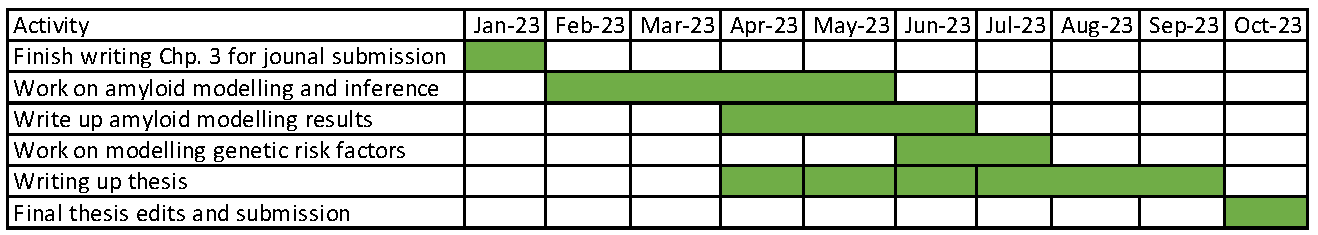
\includegraphics[width=1.0\textwidth]{gant.pdf}
    \caption{\textbf{Future work and submission timetable}}
    \label{fig:stupid-gant-chart}
\end{figure}
%now enable appendix numbering format and include any appendices
% \appendix
% \include{appendix1}
% \include{appendix2}

%next line adds the Bibliography to the contents page
\addcontentsline{toc}{chapter}{Bibliography}
%uncomment next line to change bibliography name to references
%\renewcommand{\bibname}{References}
% \bibliography{refs}        %use a bibtex bibliography file refs.bib
% \bibliographystyle{plain}  %use the plain bibliography style

\printbibliography
% \bibliographystyle{unsrt}
% \bibliography{refs}
\end{document}